% ====================================================================
% ★ release 1.0.14 (2026-07-04) — graphite_ica_ch1_v1.0.14.tex (계보 1.0.13 승계)
%   = 1.0.10/1.0.11 기반 + Fable 전수 재검(docs/Fable_점검 감사 ①②③) 반영:
%     물리 주장 정정(H-1 Ch2 연동·H-2 w_j 지위)·서술/귀속 정정(M-1~M-11)·LCO 6절 수식화(P1.1 supplement 계승).
%     코드 Anode_Fit 1.0.14 와 동일 버전·matched.
% --------------------------------------------------------------------
% (계보 이력) release 1.0.10 (2026-07-01) — v10-11 내용 + 버전 1.0.10 라벨.
%   adversarial 2-에이전트 재검수(문건 물리·코드정합·그래프; 확정 CRIT/HIGH 0) 후 가독성 4-다리 보강:
%     (1) Maxwell 공통접선=공통 전위 값 ↔ Dreyer 순차전환=실현 경로 화해 (sec:broadening (a))
%     (2) 두-상 내재폭 절에 "현재 코드 n_j=1 고정→실폭 RT/F≈25.7mV, 'w' 폴백은 'n' 제거 시 활성" 명시 (오독 차단)
%     (3) w 초기값 시제 명확화("전부 두-상"=초기값일 뿐, 피팅 후 전이별로 갈림) (sec:width)
%     (4) solid-solution 전이↔표 tab:staging 행(4→3·3→2L) 라벨 브리지
%   물리·부호·식 불변. 전자엔트로피 절은 v9 원문 위 additive 정련(삭제 0·물리 무손실 — 종전 "byte-identical" 기록은
%   1.0.10 정련분 반영 전 표기라 정정함, Fable 감사 H-1 인계). 코드 정상 종개형 = results/code/figs/.
% --------------------------------------------------------------------
% graphite_ica_ch1_v8-11.tex — Chapter 1 (v8-11: 유도 확장판 9+9+1+1 최종본)
%   v8-10(체리픽) 을 adversarial 재검수(Phase6, 확정 CRIT/HIGH 0) 후 LOW 폴리시 보강한 최종.
%   보강: eq:Veq 출발 다리 가시화·fig:relaxode 캡션 정리(작가메모 제거)·z_cut 선택값 명시.
%   v10-10 (base=v10-06; 사용자 2차 명확화 반영): broadening 절(sec:broadening, fig:broadening) + w 이중지위(sec:width)
%     broadening 3기작 = ①유한율속 비대칭 꼬리(L_V, fly2020) ②내재 RT/F(leviaurbach1999)
%       ③★집합 다입자 통계역학(앙상블 ρ(U_j) 전이전위 분포·비-크기 구조무질서·dahn1995·dreyer2010; forward ∫ρ·응답=eq:ensavg; ρ→δ 환원).
%     ★사이즈(반경) 효과 전면 배제(τ∝r²·반경→U_j·PSD 크기 convolution·cogswell2012 드롭). 범위경고=사이즈 동역학·반경→평형U·PSD 안 다룸.
%     Ω/two-phase 재정합: two-phase=LiC₁₂·LiC₆ 2개만(코드 Ω 초기값 전부>2RT=거친 추정·피팅 시 solid-solution은 Ω<2RT).
%     forward-only(ρ(U_j) 역산 안 함·ill-posed). w_eff 완전제거 유지. 인용 정정: +dahn1995·dreyer2010, -cogswell2012(size). [v10-11 supersede: ρ(U_j)→ρ(U_app)·fly2020=A.Fly·R.Chen(종전 Schaltz/vol.29 표기 오류) — 아래 v10-11 블록 참조]
%     + w_eff 제거(eq:weff·func_w_eff·use_w_eff·w_eff_floor_frac 자취 0; two-phase 실측은 종이지 델타 아님 — narrowing 반대방향).
%     v9 흑연·LCO 전자엔트로피·ξ_eq 분포·부호·그림 전부 보존.
%   v10-11 (base=v10-10; adversarial A1/A3 정정): ★기작③(집합 통계역학) 재정초 —
%     (iii-a) Dreyer 다입자 *평형* 통계역학 = plateau 구조(순차 전환·공통 전위) 기원,
%     (iii-b) plateau→실측 broadening = 앙상블 apparent-U=U_j+η 분포. forward 적분변수 ρ(U_j)→ρ(U_app),
%       U_app=U_j+η. ★평형 중심 U_j=입자 무관 상수(분포≈0), 분포하는 건 η(과전압·국소환경, 비-크기).
%       → "중심 상수↔폭(η) 분포" 모순 해소(ORIGIN §3 정합). ρ→δ 면 평형 중심 단일 델타 환원.
%     기작③ = 흑연 two-phase(LiC₁₂·LiC₆)에 scope(LCO 는 일반 η 분포만). dahn1995 = intra-particle 용량한계
%       예시·tier C(inter-particle ρ 1차근거 아님). ①(kinetic L_V) vs ③(앙상블 η 통계평균) 분리 서술.
%     A3: fig:broadening 본문 \ref 추가(orphan 해소). 인용 정정(Crossref 확정) —
%       fly2020 = A.Fly·R.Chen(2인, "Rate dependency of ICA…", DOI .est.2020.101329 — 종전 Schaltz/Stroe·2019 오류 교정),
%       dahn1995 = Dahn·Zheng·Liu·Xue 표준 서지, rsc2021 = Onuma 외 9인(K-graphite 주제, Li-staging 비교 인용·tier B).
%     전자엔트로피 절 v9 대비 additive 정련(1.0.10에서 교차검증·단위박스 추가 — "byte-identical/SHA 불변"은 그 전 시점 표기)·w_eff 잔존 0·사이즈 제외·Ω/two-phase 2개 유지.
%   불가침: 부호 8/8·11식 G-derive(SymPy/NumPy 검증)·D-PEAK/D-PEAK2·D-WEFF·결과 박스·코드 정합·그림 9.
%   ── 이하 v8-10(= v8-06b 베이스) 원형 ──
% graphite_ica_ch1_v8-10.tex — Chapter 1 (v8-10: 유도 확장판 9+9 경쟁·검토 체리픽 통합본)
%   베이스 = v8-06b(검토2 34/35·전 KNOWN_DEFECTS 해소·D-PEAK 2곳 정확·9 figs), v6 합류 교차검증.
%   보강 = D-PEAK2(eq:branch 문턱 진폭 불연속 = 이산 모드 스위치 정직 기술).
%   그림 경쟁 승자 = v7-11 유래 5 + 신규 4(검토2 청정). 이식금지 회귀: v8-02/03 D-PEAK 재정정·D-WEFF ¼·v8-07 s_F orphan.
%   ── 이하 베이스 v8-06b 원형 ──
% graphite_ica_ch1_v8-06.tex — Chapter 1 (v8-06: 유도 과정 포함 교과서 확장판)
%   배치·결과 박스·식별자·부호·표 = v7-11.tex 보존(절 순서 N0->N9·결과 박스 9식·
%   그림 5개·표 3종·부호 검산 절). v7 가 압축한 중간 유도를 v5 유도 원천에서
%   가져와 이 배치에 맞춰 다시 전개(베끼지 않음) — 각 결과 박스 위에
%   (a) 출발식/전제 -> (b) 적용 연산 -> (c) 중간식 >=1 -> (d) 박스 의 단계가 보인다.
%   유도 원천 = graphite_ica_ch1_Opus_v5.tex(통계역학 전 유도). 결과·부호 정본 =
%   Anode_Fit_v1.0.14.py(계보 v11_final→use_w_eff 제거→1.0.10→1.0.12→1.0.13→1.0.14). 무관 일반론(lever/chord·Marcus·KWW·적층·
%   master 알고리즘 S0-S5)은 결과 박스로 수렴하지 않으므로 재유입 안 함.
%   그림 = v7-11 의 5개(spine·staging·hysloop·logistic·reversal) 보존 + 유도를
%   돕는 신규 4개(activation barrier·flux crossing·double-well·relaxation ODE).
%   내부 텍스트 영어 ASCII 만.
%   build: xelatex -interaction=nonstopmode 2-pass (kotex — 한글 전제).
% ====================================================================
\documentclass[11pt,a4paper]{article}
\usepackage[margin=22mm]{geometry}
\usepackage{kotex}
\setmonofont{D2Coding}[Scale=MatchLowercase]
\usepackage{amsmath,amssymb,mathtools,bm}
\usepackage{booktabs,longtable,array}
\usepackage{enumitem}
\usepackage{amsthm}
\usepackage{hyperref}
\usepackage{fancyhdr}
\usepackage{lastpage}
\usepackage{setspace}
\usepackage{tikz}
\usetikzlibrary{positioning,arrows.meta,calc,fit,backgrounds}
\setstretch{1.12}
\setlength{\parskip}{0.45em}\setlength{\parindent}{0pt}\setlength{\headheight}{14pt}
\setlength{\emergencystretch}{2em}
\hypersetup{colorlinks=true, linkcolor=blue, urlcolor=blue, citecolor=blue,
  pdftitle={흑연 음극 + LCO 양극 dQ/dV 이론: 코드 진행을 따라가는 수식-구동 (유도 확장) — Chapter 1 (v1.0.14)}}
\pagestyle{fancy}\fancyhf{}
\lhead{흑연 음극 + LCO 양극 $dQ/dV$ 이론 — Ch.1 (v1.0.14, 통계역학-first + 코드 진행)}\rhead{\thepage/\pageref{LastPage}}
\renewcommand{\headrulewidth}{0.4pt}

\newtheorem*{keybox}{핵심}
\newtheorem*{codebox}{코드 대응}
\newtheorem*{signbox}{부호 검산}
\newtheorem*{verifybox}{검산}
\newtheorem*{derivbox}{유도}

\newcommand{\dd}{\mathrm{d}}
\newcommand{\eff}{\mathrm{eff}}
\newcommand{\eq}{\mathrm{eq}}
\newcommand{\app}{\mathrm{app}}
\newcommand{\cell}{\mathrm{cell}}
\newcommand{\bg}{\mathrm{bg}}
\newcommand{\rxn}{\mathrm{rxn}}
\newcommand{\dis}{\mathrm{dis}}
\newcommand{\chg}{\mathrm{chg}}
\newcommand{\hys}{\mathrm{hys}}
\newcommand{\work}{\mathrm{work}}
\newcommand{\rep}{\mathrm{rep}}
\newcommand{\code}[1]{\texttt{#1}}

\renewcommand{\theequation}{1.\arabic{equation}}
\renewcommand{\thesection}{1.\arabic{section}}
\title{\textbf{\LARGE Chapter 1}\\[0.35em]\Large 흑연 음극 + LCO 양극 $dQ/dV$ 이론: 한 곡선을 그리는 코드 진행을 따라가는 수식-구동판 — 유도 확장}
\author{}
\date{\normalsize 버전 1.0.14 \quad(코드 \texttt{Anode\_Fit 1.0.14} 와 동일 버전 · matched)}

\makeatletter
\renewcommand*\l@section[2]{%
  \ifnum \c@tocdepth >\z@
    \addpenalty\@secpenalty
    \addvspace{1.0em \@plus\p@}%
    \setlength\@tempdima{2.3em}%
    \begingroup
      \parindent \z@ \rightskip \@pnumwidth
      \parfillskip -\@pnumwidth
      \leavevmode \bfseries
      \advance\leftskip\@tempdima
      \hskip -\leftskip
      #1\nobreak\hfil
      \nobreak\hb@xt@\@pnumwidth{\hss #2\kern-\p@\kern\p@}\par
    \endgroup
  \fi}
\renewcommand*\l@subsection{\@dottedtocline{2}{2.3em}{3.2em}}
\makeatother

\begin{document}
\maketitle

% ====================================================================
\section*{서론 — 이 문건이 따라가는 것}
\addcontentsline{toc}{section}{서론}
% ====================================================================
리튬이온전지 흑연 음극의 incremental capacity analysis(ICA)는 충방전 곡선 $Q(V)$ 의 미분
$\dd Q/\dd V$ 를 본다 \cite{bloom2005,dubarry2012}. 흑연은 staging 상전이(stage
$4\!\to\!3\!\to\!2\mathrm L\!\to\!2\!\to\!1$)를 거치며 \cite{dahn1991,ohzuku1993}, 각 전이 전위에서
두 상이 공존하면 전위가 거의 평탄해 좁은 $\dd V$ 에 큰 $\dd Q$ 가 몰려 $\dd Q/\dd V$ 가 치솟는다.

본 문건은 이 곡선을 \emph{한 번 그리는 계산}을 그대로 따라간다. 계산은 외부 실험조건 환산(N0)$\to$전이별
물리식 평가(N1--N9)의 순서를 밟는다(그림~\ref{fig:spine}). 각 절은 그 한 단계의 물리식을, 그 단계를 이해하는 데 필요한 만큼
\emph{유도}한다 — 결과식만 나열하지 않고, 출발 전제에서 그 식까지 가는 중간 단계를 빠짐없이 보인다. 곡선에 들어가지 않는 일반론은 결과식이 쓰이는 한에서만 최소로 인용한다. 도착점은 한 줄
합산식과, ``이 문건만 보고 같은 곡선을 재현하는 코드를 짤 수 있다''는 실행 가능성이다. 본론에 앞서 Part 0
(\S\ref{sec:sm-found})이 이 사슬의 평형식들을 통계역학 첫 원리(분배함수)에서 유도해 두고, 본론 N1--N9 가 흑연
사슬을 닫은 뒤 Part II(\S\ref{sec:lco-intro})가 같은 골격을 두 번째 전극 LCO 양극에 건다 — MSMR(multi-species,
multi-reaction) 동형에 전자 엔트로피 항 하나를 더한 확장이다. 문서는 Part 0 $\to$ 흑연(Part I) $\to$ Part II 세 층이다.

\textbf{관측.}
\begin{quote}\itshape
$\dd Q/\dd V$ 상전이 peak 의 위치$\cdot$너비$\cdot$높이는 (a) 온도 $T$, (b) 극판 전위, (c) C-rate(전류)
세 가지에 따라 변한다. 저온$\cdot$고율일수록 peak 의 꼬리가 길어져 다음 peak 와 겹치고, 같은 전이가 충전과 방전에서
서로 다른 전위에 peak 를 남기며(충방전 히스테리시스 — 이하 `히스'로도 축약), 이 갈림에는 전류를 $0$ 으로 줄여도 사라지지 않는 성분이 있다.
\end{quote}

세 인자는 모두 하나의 속도식 $k\simeq k_0\exp[-\Delta G_a/RT]$ 의 서로 다른 자리로 들어온다 — 온도는 지수의 분모,
전위는 장벽 $\Delta G_a$ 자체, C-rate 는 요구 속도와 공급 속도의 경쟁이다. 이 속도식이 한편으로는 평형(정$\cdot$역
속도가 같아지는 정지점)을, 다른 한편으로는 유한 전류의 지연(꼬리)을 낳는다 — 본 문건의 유도는 줄곧 이 한 식의 가지를
펼치는 일이다. 코드 진행이 이 세 갈래를 차례로 닫는다.

\begin{figure}[t]
\centering
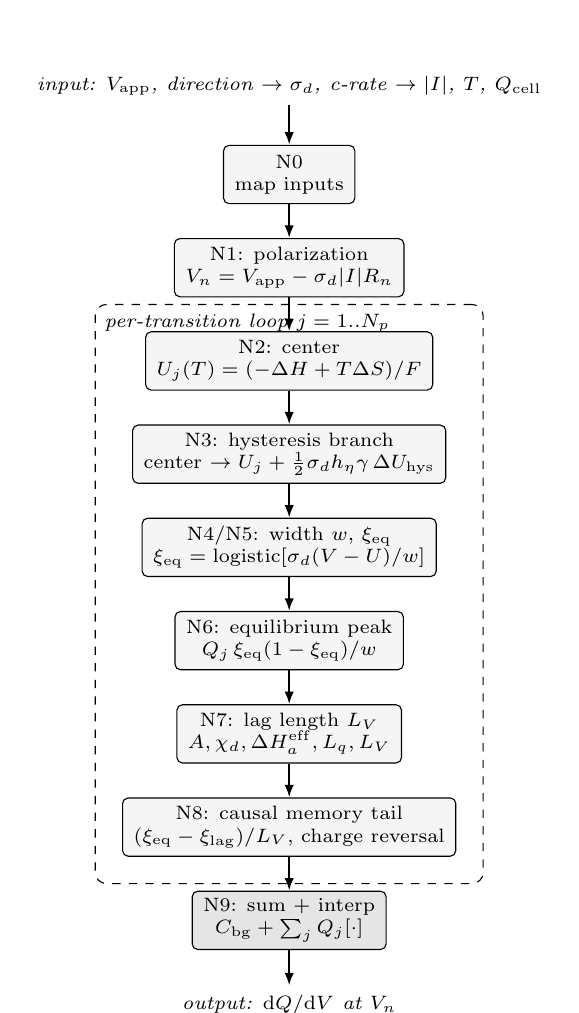
\begin{tikzpicture}[
  node distance=4.3mm and 5.5mm,
  stage/.style={draw,rounded corners=2pt,minimum height=7.4mm,inner xsep=4pt,inner ysep=2.5pt,font=\scriptsize,align=center,fill=black!4},
  core/.style={stage,fill=black!10},
  io/.style={font=\scriptsize\itshape,align=center},
  ar/.style={-{Latex[length=1.6mm]},thick}]
% input row
\node[io] (in) {input: $V_\app$, direction $\to\sigma_d$, c-rate $\to|I|$, $T$, $Q_\cell$};
% spine
\node[stage,below=5mm of in] (n0) {N0\\map inputs};
\node[stage,below=of n0] (n1) {N1: polarization\\$V_n=V_\app-\sigma_d|I|R_n$};
\node[stage,below=of n1] (n2) {N2: center\\$U_j(T)=(-\Delta H+T\Delta S)/F$};
\node[stage,below=of n2] (n3) {N3: hysteresis branch\\center $\to U_j+\tfrac12\sigma_d h_\eta\gamma\,\Delta U_\hys$};
\node[stage,below=of n3] (n4) {N4/N5: width $w$, $\xi_\eq$\\$\xi_\eq=\mathrm{logistic}[\sigma_d(V-U)/w]$};
\node[stage,below=of n4] (n6) {N6: equilibrium peak\\$Q_j\,\xi_\eq(1-\xi_\eq)/w$};
\node[stage,below=of n6] (n7) {N7: lag length $L_V$\\$A,\chi_d,\Delta H_a^\eff,L_q,L_V$};
\node[stage,below=of n7] (n8) {N8: causal memory tail\\$(\xi_\eq-\xi_\mathrm{lag})/L_V$, charge reversal};
\node[core,below=of n8] (n9) {N9: sum + interp\\$C_\bg+\sum_j Q_j[\cdot]$};
\node[io,below=4.5mm of n9] (out) {output: $\dd Q/\dd V$ at $V_n$};
\foreach \a/\b in {in/n0,n0/n1,n1/n2,n2/n3,n3/n4,n4/n6,n6/n7,n7/n8,n8/n9,n9/out}
  \draw[ar] (\a) -- (\b);
% per-transition loop bracket
\begin{scope}[on background layer]
\node[draw,dashed,rounded corners,fit=(n2)(n3)(n4)(n6)(n7)(n8),inner sep=3.4mm,label={[font=\scriptsize\itshape,anchor=north west]north west:per-transition loop $j=1..N_p$}] (loop) {};
\end{scope}
\end{tikzpicture}
\caption{한 곡선을 그리는 계산 진행(spine). 외부 실험조건 $(\sigma_d,|I|,T,Q_\cell)$
이 N0 에서 모델 입력으로 환산되고, 분극으로 내부 전위 $V_n$ 을 얻은 뒤(N1), 전이 $j$ 마다 평형 중심$\cdot$히스
분기$\cdot$폭$\cdot$평형 진행률$\cdot$평형 peak$\cdot$지연 길이$\cdot$인과 꼬리를 계산해(N2--N8) 합산$\cdot$역보간한다(N9).
파선 상자는 전이별 반복 계산 단위다.}
\label{fig:spine}
\end{figure}

\tableofcontents
\newpage

% ====================================================================
\section{기호와 규약, 실험조건 매핑 (N0)}\label{sec:notation}
% ====================================================================
계산의 진입점은 실험조건 $(V_\app,\text{direction},\text{c\_rate},Q_\cell,T)$ 을 받아 그 첫 일로 이를 모델
입력으로 환산하는 것이다 — 이것이 노드 $\mathrm N0$ 다. 방향 문자열은 방향 부호 $\sigma_d$ 로,
C-rate 는 전류 크기 $|I|$ 로 바뀐다:
\begin{equation}
\sigma_d=\begin{cases}+1 & \text{방전(discharge)}\\ -1 & \text{충전(charge)}\end{cases},
\qquad
|I|=\text{c\_rate}\cdot Q_\cell\quad(\text{또는 }I_\mathrm{abs}\text{ 직접 지정}).
\label{eq:n0map}
\end{equation}
c\_rate 는 시간 역수이므로 $Q_\cell$ 과 시간 단위를 맞춰 대입한다([1/h]$\cdot$[A\,h]$\to$[A]; 코드 규격화
$Q_\cell{=}1$ 에서는 무차원 배율). 방향 부호의 작용처는 셋이다 — 분극 부호($\mathrm N1$)$\cdot$분기 중심 선택($\mathrm N3$)$\cdot$꼬리($\mathrm N7\cdot\mathrm N8$:
방향별 전달계수 $\chi_d$ 가 꼬리 \emph{길이}를, 격자 역전이 인과 기억의 진행 \emph{방향}을 가른다).
평형 종 자체는 방향 불변이다(아래에서 식으로 회수). 본 장이 뽑는 양은 $\dd Q/\dd V$ 한 곡선이다.

\textbf{전이 인덱스.} $j=1,\dots,N_p$($N_p\approx3$--$4$). 전이 $j$ 의 진행률 $\xi_j$(방전 시 $0\to1$ 로 증가, 곧 탈리튬화 진행),
용량 가중 $Q_j$. 박스 결과식은 $j$ 첨자를 단다. 점유율과 진행률은 $\theta_j=1-\xi_j$ 로 묶이며(점유 $\theta$ 가 $1\to0$
줄어드는 것이 진행 $\xi$ 가 $0\to1$ 느는 것), 유도에서 둘은 부호 한 번 차이로 오간다.

\textbf{부호 규약(★최우선 결함 클래스).} 전위는 흑연 음극 반쪽전지 전위(vs Li/Li$^+$)다. 방향 부호 $\sigma_d=\pm1$
(방전 $+1$/충전 $-1$)이며, 평형 진행률 $\xi_\eq=\mathrm{logistic}[\sigma_d(V-U)/w]$ 에서 방전
($\sigma_d=+1$)은 $V\!\uparrow\Rightarrow\xi_\eq\!\uparrow$(전위를 올리면 탈리튬화). 분기 중심 $+\tfrac12\sigma_d(\cdots)$
는 $\sigma_d$ 를 따라 방전$\cdot$충전이 반대로 갈리고, 꼬리는 충전에서 격자 역전을 받는다. 이 규약은 \S\ref{sec:notation}--\S\ref{sec:sum}
과 Part II 전건에서 유지되며 \S\ref{sec:signcheck} 가 전수 검산한다.

\begin{longtable}{p{0.15\textwidth} p{0.16\textwidth} p{0.605\textwidth}}
\toprule 기호 & 단위 & 의미 \\ \midrule \endhead
\multicolumn{3}{l}{\emph{— 실험조건$\cdot$방향(N0$\cdot$N1) —}}\\
$\sigma_d$ & --- & 방향 부호 — 방전 $+1$/충전 $-1$ \\
$s$ & --- & 유도 전용 고정 부호 — 항상 $+1$(\S\ref{sec:center}$\cdot$\S\ref{sec:hys} 의 $U_j$ 정의 관례); 방향에 따라 $\pm1$ 로 바뀌는 $\sigma_d$ 와 별개, 본론 결과-사슬 boxed 식에서 $s{=}1$ 대입돼 소멸(Part 0 의 박스는 $s$ 를 명시 유지) \\
$|I|$ & A & 전류 크기 $=$ c-rate$\,\cdot Q_\cell$ \\
$Q_\cell$ & C(또는 A\,h) & 셀 용량(전하); $q=Q/Q_\cell$ 환산$\cdot$$|I|$ 환산 공용 — $|I|$ 환산 시 c-rate 와 시간 단위 정합 \\
$T$ & K & 온도 — 스칼라(등온) 또는 $V_\app$ 길이 배열($T(V)$ 비등온) \\
$R_n$ & $\Omega$ & 음극 lumped 분극 저항 \\
$V_\app$ & V & 인가(측정) 전위 격자 \\
$V_n$ & V & 내부(열역학) 전위 $=V_\app-\sigma_d|I|R_n$ \\
\multicolumn{3}{l}{\emph{— 평형 중심$\cdot$폭$\cdot$진행률(N2$\cdot$N4$\cdot$N5) —}}\\
$U_j(T)$ & V & 전이 $j$ 평형 중심 전위 $=(-\Delta H_\rxn+T\Delta S_\rxn)/F$ \\
$\Delta H_{\rxn,j},\Delta S_{\rxn,j}$ & {\footnotesize J/mol;\,J/(mol\,K)} & 삽입 \emph{반응} 엔탈피$\cdot$엔트로피(평형 — \emph{활성화}와 다름) \\
$n_j$ & --- & 폭 다중도($w=n_jRT/F$; 폭 $w$ 를 직접 주면 $n=wF/RT$ 역산) \\
$w_j$ & V & 전이 폭 척도 $=n_jRT/F$ \\
$\xi_{\eq,j}$ & --- & 평형 진행률(logistic) \\
$Q_j$ & C & 전이 $j$ 용량 가중 \\
$C_\bg$ & C/V & 배경 미분용량(상수 또는 $V$ 함수) \\
\multicolumn{3}{l}{\emph{— 히스테리시스 분기(N3) —}}\\
$\Omega_j$ & J/mol & 정규용액(regular solution) 상호작용 에너지($>2RT$ 면 상분리$\cdot$히스) \\
$\gamma_j$ & --- & 분기 축소 인자 $0\le\gamma_j\le1$($0$ 이면 분기 없음) \\
$\Delta U_j^\hys$ & V & spinodal 상한 분기 gap \\
$h_{\eta,j}$ & --- & 부분 cycle 인자(기본 $1$) \\
$U_j^{\,d}$ & V & 방향별 분기 중심 \\
\multicolumn{3}{l}{\emph{— 동역학 꼬리(N7$\cdot$N8) —}}\\
$\chi$ & --- & 전이상태 분율 위치(전달 계수); 방향별 $\chi_d$ \\
$\chi_d$ & --- & 방향별 전달 계수 — 방전 $\chi$/충전 $1-\chi$ \\
$\mathcal A_j$, $\mathcal A$ & J/mol & affinity(구동력) — 첨자형 $\mathcal A_j=sF(V-U_j)$ 는 유도용
일반 구동력(\S\ref{sec:width}; N7 일반형은 $-\Omega_j(1-2\xi_j)$ 가 더해짐), 무첨자 $\mathcal A$ 는
꼬리 컷점에 동결한 값 $=\min(z_\mathrm{cut}n_jRT,\,A_\mathrm{cap}RT)$(\S\ref{sec:lag}) \\
$\Delta H_{a,j},\Delta S_{a,j}$ & {\footnotesize J/mol;\,J/(mol\,K)} & \emph{활성화} 엔탈피$\cdot$엔트로피(속도) \\
$\Delta H_{a,j}^\eff$ & J/mol & 유효 장벽 $=\Delta H_a-\chi_d\Omega$ \\
$L_{q,j}$ & --- & 용량축 지연 길이 \\
$L_{V,j}$ & V & 전압축 지연 길이 $=|\dd V/\dd q|_{q_a}L_{q,j}$ \\
$|\dd V/\dd q|_{q_a}$ & V & 컷점 OCV(open circuit voltage) 기울기($L_q\to L_V$ 환산) \\
$z_\mathrm{cut}$ & --- & 컷 affinity 의 $z=\mathcal A/(n_jRT)$(기본 $4.357$) \\
$A_\mathrm{cap}$ & --- & 컷 affinity 상한 배수(기본 $4.0$) \\
$\xi_{\mathrm{lag},j}$ & --- & 인과 저역통과된 진행률 \\
\multicolumn{3}{l}{\emph{— 상수 —}}\\
$R,F,k_B,h$ & {\footnotesize J/(mol\,K), C/mol, J/K, J\,s} & 기체상수, Faraday, Boltzmann, Planck \\
\bottomrule
\end{longtable}

물리 기호와 구현 식별자의 대응은 부록~\ref{sec:appendix-code}(표~\ref{tab:symcode})에 정리한다.

흑연 staging 의 갤러리 채움을 그림~\ref{fig:staging} 에 둔다 — 각 stage 전이가 한 peak 를 남기고,
흑연 staging 네 전이의 초기값(문헌 기반, 표~\ref{tab:staging})이 이 네 전이에 대응한다.

\begin{figure}[t]
\centering
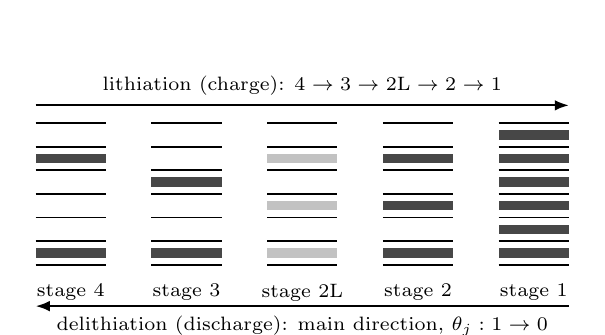
\begin{tikzpicture}[x=1.05cm,y=0.5cm,
  lab/.style={font=\scriptsize,align=center},
  fill4/.style={fill=black!72},fillL/.style={fill=black!24}]
% five stage columns, each shows graphene layers (lines) and Li-filled galleries (bands)
% column x-centers
\def\colw{0.85}
% stage 4: 1 filled gallery of 4
\foreach \x/\name/\filled/\style in {0/{stage 4}/{1}/fill4, 1.4/{stage 3}/{1}/fill4, 2.8/{stage 2L}/{all}/fillL, 4.2/{stage 2}/{all}/fill4, 5.6/{stage 1}/{dense}/fill4}{
  \draw[semithick] (\x,0)--(\x+\colw,0);
  \foreach \k in {1,2,3,4,5,6}{\draw[semithick] (\x,0.6*\k)--(\x+\colw,0.6*\k);}
  \node[lab,below] at (\x+\colw/2,-0.25) {\name};
}
% galleries (bands between layers) — explicit per column for clarity
% stage 4: every 4th gallery filled
\foreach \k in {1,5}{\fill[black!72] (0,0.6*\k-0.42) rectangle (0+\colw,0.6*\k-0.18);}
% stage 3: every 3rd
\foreach \k in {1,4}{\fill[black!72] (1.4,0.6*\k-0.42) rectangle (1.4+\colw,0.6*\k-0.18);}
% stage 2L: every 2nd, light (liquid-like)
\foreach \k in {1,3,5}{\fill[black!24] (2.8,0.6*\k-0.42) rectangle (2.8+\colw,0.6*\k-0.18);}
% stage 2: every 2nd, dark
\foreach \k in {1,3,5}{\fill[black!72] (4.2,0.6*\k-0.42) rectangle (4.2+\colw,0.6*\k-0.18);}
% stage 1: all galleries
\foreach \k in {1,2,3,4,5,6}{\fill[black!72] (5.6,0.6*\k-0.42) rectangle (5.6+\colw,0.6*\k-0.18);}
\draw[-{Latex[length=1.8mm]},thick] (0,4.05)--(6.45,4.05) node[pos=0.5,above,font=\scriptsize] {lithiation (charge): $4\to3\to2\mathrm L\to2\to1$};
\draw[{Latex[length=1.8mm]}-,thick] (0,-1.05)--(6.45,-1.05) node[pos=0.5,below,font=\scriptsize] {delithiation (discharge): main direction, $\theta_j:1\to0$};
\end{tikzpicture}
\caption{흑연 staging 의 갤러리 채움 도식. 수평선이 그래핀 층, 음영 띠가 리튬이 든 층간 갤러리다.
채울수록 stage 번호가 줄어 stage 1($\mathrm{LiC_6}$, 완전 채움)에 닿고, 각 stage 전이가 $\dd Q/\dd V$ 에 peak
하나를 남긴다. stage $2\mathrm L$ 은 면내 질서가 풀린 단계라 옅게 표시했다. 코드의 전이 리스트 4건이 이 전이들의
초기값이며($U\approx0.21/0.14/0.12/0.085$ V), 본 문건 방향은 방전(탈리튬화)이다.}
\label{fig:staging}
\end{figure}

이 골격의 두 번째 전극(LCO 양극) 일반화는 Part II(\S\ref{sec:lco-intro})가 연다. 그 전에, 본론 결과 사슬이
결과로만 받아 쓰는 평형식들($\theta$-점유·logistic·평균장 $\Omega$·Nernst)의 통계역학 유도를 바로 다음 절
Part 0 이 처음부터 놓는다.

% ====================================================================
% ★ Part 0 신설(v1.0.14 P2.1 통합본) — 통계역학 기초.
%   배치: N0(sec:notation) 말미(현행 L300, fig:staging 뒤) 직후 · N1(sec:pol) 앞.
%   신설 라벨 eq:sm-* / 이동 편입 라벨(원위치 정의 삭제 필수) = eq:partfn·eq:fermifn·eq:mu·eq:gxi.
% ====================================================================
\section{통계역학 기초 --- 분배함수에서 Nernst 식까지 (P0)}\label{sec:sm-found}

본론(N1--N9)의 모든 평형식은 통계역학의 한 사슬에서 나온다. 이 절은 그 사슬을 처음부터 놓으며, 통계역학
사전지식 없이도 본론의 출발점들이 이 절 안에서 닫히도록 각 단계를 (a) 출발 $\to$ (b) 연산 $\to$ (c) 중간식
$\to$ (d) 박스로 전개한다. 유도의 골격은 고전 통계역학(분배함수$\cdot$화학퍼텐셜)으로 닫히고, 양자 통계가
필요한 항(점유 자리의 진동 자유도, Chapter 2 의 포논$\cdot$전자 분포)은 해당 자리에서 명시적으로 도입한다.
사슬은
\[
\boxed{\;\begin{aligned}
&\text{미시상태·앙상블}\ \to\ Z,\Xi\ \to\ \theta=\frac{1}{1+e^{\beta(\tilde\varepsilon-\mu)}}\ \to\ \text{lattice gas}\\
&\to\ \mu(\theta;\Omega)\ \to\ \xi_\eq\ \text{logistic}\ \to\ G,\ \text{Nernst}
\end{aligned}\;}
\]
이고, 도착점들이 본론 결과 사슬 --- \S\ref{sec:center} 의 $U_j(T)$, \S\ref{sec:hys} 의 히스테리시스,
\S\ref{sec:width} 의 $\xi_\eq$ --- 의 입력이다.

\subsection{앙상블과 Boltzmann·Gibbs 인자 --- 분배함수와 화학퍼텐셜 $\mu$}\label{sec:sm-ensemble}
\textbf{(a) 출발 --- 미시상태·앙상블과 두 공준.} \emph{미시상태}(microstate)는 계의 모든 자유도를 지정한
배치 하나이고, \emph{거시상태}(macrostate)는 에너지·부피·입자수 $(E,V,N)$ 같은 소수의 거시변수만 지정한
미시상태의 집합이다. 같은 거시 조건을 공유하는 미시상태들의 모음이 \emph{앙상블}(ensemble)이다. 통계역학은
두 공준으로 시작한다 --- 고립계 평형에서 접근 가능한 $W$ 개 미시상태는 등확률이고(공준 1), 엔트로피는 그
경우의 수의 로그다(공준 2, Boltzmann):
\begin{equation}
S\;=\;k_B\ln W.
\label{eq:sm-S}
\end{equation}
열역학과의 접점은 근본 미분식 $\dd E=T\dd S-P\dd V+\mu\,\dd N$ 을 $S$ 에 대해 푼 형태다:
\begin{equation}
\dd S=\frac{1}{T}\,\dd E+\frac{P}{T}\,\dd V-\frac{\mu}{T}\,\dd N
\quad\Longrightarrow\quad
\frac{\partial S}{\partial E}\Big|_{V,N}=\frac1T,\qquad
\frac{\partial S}{\partial N}\Big|_{E,V}=-\frac{\mu}{T}.
\label{eq:sm-fund}
\end{equation}
여기서 $\mu$ 의 물리적 의미가 이미 보인다 --- 입자 1개를 받아들일 때 엔트로피가 $\mu/T$ 만큼 \emph{감소}하는
값비쌈의 척도다. 두 계 1,2 가 입자를 교환하면 총 엔트로피 변화가
$\dd S_\mathrm{tot}=\big(\tfrac{\mu_2}{T}-\tfrac{\mu_1}{T}\big)\dd N_1\ge0$ 이므로 입자는 $\mu$ 가 높은 쪽에서
낮은 쪽으로 흐르고, 정지 조건은 $\mu_1=\mu_2$ --- 화학퍼텐셜의 일치가 곧 입자 교환 평형이다.

\textbf{(b) 연산 --- 저장조와 접촉한 작은 계.} 관심 계가 거대한 저장조(reservoir)와 에너지·입자를 교환한다.
계가 미시상태 $i$(에너지 $E_i$, 입자수 $N_i$)에 있을 확률은 공준 1 에 의해 그때 저장조가 가질 수 있는 경우의
수에 비례한다:
\begin{equation}
P_i\;\propto\;W_R(E_\mathrm{tot}-E_i,\,N_\mathrm{tot}-N_i)
\;=\;\exp\!\Big[\frac{S_R(E_\mathrm{tot}-E_i,\,N_\mathrm{tot}-N_i)}{k_B}\Big].
\label{eq:sm-resv}
\end{equation}
저장조가 계보다 훨씬 크므로 $S_R$ 을 1차에서 절단해 전개하면(식~\eqref{eq:sm-fund} 의 두 도함수 대입)
\begin{equation}
S_R(E_\mathrm{tot}-E_i,\,N_\mathrm{tot}-N_i)
= S_R(E_\mathrm{tot},N_\mathrm{tot})-\frac{E_i}{T}+\frac{\mu N_i}{T}+\mathcal O(E_i^2,N_i^2).
\label{eq:sm-taylor}
\end{equation}
\textbf{(c) 중간식 --- Gibbs 인자와 canonical 특수형.} 식~\eqref{eq:sm-taylor} 을 \eqref{eq:sm-resv} 에 넣으면
상수 몫이 규격화로 빠지고
\begin{equation}
P_i\;\propto\;e^{-\beta(E_i-\mu N_i)},\qquad \beta\equiv\frac{1}{k_BT}
\label{eq:sm-gibbsfactor}
\end{equation}
--- 이 지수가 \emph{Gibbs 인자}다. 입자 교환이 없으면($N_i$ 고정) $e^{-\beta E_i}$ 의 \emph{Boltzmann 인자}로
줄고, 그 규격화 합이 canonical 분배함수(partition function) $Z=\sum_ie^{-\beta E_i}$, 그 로그가 Helmholtz
자유에너지 $F=-k_BT\ln Z$ 다($\langle E\rangle=\partial(\beta F)/\partial\beta$·$S=-\partial F/\partial T$ 가
열역학 관계와 일치함이 이 명명의 근거다). 이 $F$ 는 Faraday 상수 $F$ 와 기호만 같고 문맥으로 갈린다 —
전자는 $\partial F/\partial T$ 처럼 \emph{미분당하는 자유에너지}, 후자는 $FV$·$RT/F$ 의 전하 환산
곱$\cdot$나눗셈 상수다. 식~\eqref{eq:sm-fund} 의 $\mu$ 를 $F$ 로 옮기면
$\mu=\partial F/\partial N|_{T,V}$ --- \emph{온도·부피를 고정한 채 입자 1개를 더 넣는 자유에너지 비용}이며,
이것이 본론 \S\ref{sec:center} 가 쓰는 거시 정의 $\mu=\partial G/\partial n|_{T,P}$ 와 같은 양임은
\S\ref{sec:sm-macro} 에서 닫는다.

\textbf{(d) 박스 --- grand canonical 분배함수.} 입자수까지 교환하는 앙상블이
\emph{대정준}(grand canonical) 앙상블이고, 그 규격화 합과 평균 입자수는
\begin{equation}
\boxed{\;\Xi=\sum_i e^{-\beta(E_i-\mu N_i)},\qquad
P_i=\frac{e^{-\beta(E_i-\mu N_i)}}{\Xi},\qquad
\langle N\rangle=k_BT\,\frac{\partial\ln\Xi}{\partial\mu}\;}
\label{eq:sm-gc}
\end{equation}
($\partial\ln\Xi/\partial\mu=\beta\sum_iN_iP_i=\beta\langle N\rangle$ 로 셋째 식이 첫째·둘째에서 나온다).
극한 검산 --- $\beta\to0$ 이면 $P_i\to$ 등확률(열적 규율 소실), $\beta\to\infty$ 면 $E_i-\mu N_i$ 최소 상태만
남는다. 삽입 전극이 정확히 이 설정이다 --- 격자의 자리들이 전해질을 통해 Li 저장조(상대극 Li 금속)와 입자를
교환하므로 $\mu$ 가 고정된 대정준 문제이고(그림~\ref{fig:sm-reservoir}), 다음 소절이 그 최소 단위(자리
하나)를 푼다.

\begin{figure}[t]
\centering
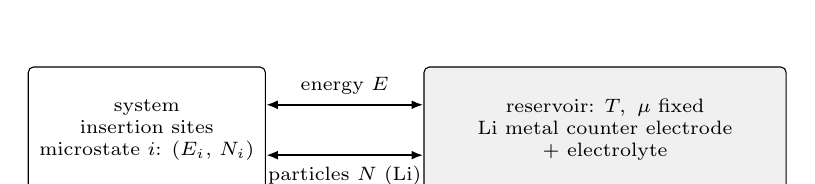
\begin{tikzpicture}[font=\scriptsize,
  box/.style={draw,rounded corners=2pt,align=center,inner sep=4pt},
  ar/.style={{Latex[length=1.5mm]}-{Latex[length=1.5mm]},thick}]
\node[box,minimum width=30mm,minimum height=16mm] (sys) {system\\insertion sites\\microstate $i$: $(E_i,\,N_i)$};
\node[box,minimum width=46mm,minimum height=16mm,fill=black!6,right=20mm of sys] (res)
  {reservoir: $T,\ \mu$ fixed\\Li metal counter electrode\\$+$ electrolyte};
\draw[ar] ([yshift=3.2mm]sys.east) -- ([yshift=3.2mm]res.west) node[midway,above] {energy $E$};
\draw[ar] ([yshift=-3.2mm]sys.east) -- ([yshift=-3.2mm]res.west) node[midway,below] {particles $N$ (Li)};
\end{tikzpicture}
\caption{grand canonical 구도. 관심 계(삽입 자리들)는 상대극$\cdot$전해질이 이루는 큰 저장조와
에너지$\cdot$입자를 모두 교환하고, 저장조는 $T$ 와 $\mu$ 를 고정한다. 에너지만 열면 Boltzmann 인자, 입자까지
열면 Gibbs 인자(식~\eqref{eq:sm-gibbsfactor}) --- 지수의 자리가 하나 늘어날 뿐 논리는 같다.}
\label{fig:sm-reservoir}
\end{figure}

\subsection{단일 삽입 자리 --- 점유 통계와 그 요동}\label{sec:sm-site}
\textbf{(a) 출발 --- 두 가정과 미시상태의 온전한 기술.} 격자의 삽입 자리 \emph{하나}를 떼어 살펴본다.
자리는 전해질 너머의 Li 저장조와 입자를 교환하므로 식~\eqref{eq:sm-gc} 의 대정준 설정 그대로다. 유도에
앞서 두 가정을 명시한다.
\begin{itemize}[leftmargin=2.2em,itemsep=0.1em]
\item \textbf{가정 1 (hard-core 배타).} 한 자리에는 Li 이온이 $0$ 개 또는 $1$ 개만 들어간다. 근거는 양자
통계가 아니라 강한 단거리 반발이다 --- 자리의 부피와 이온 사이 정전$\cdot$입체 반발이 이중 점유의
에너지를 사실상 무한대로 올린다. 이 가정이 점유수 합을 $n\in\{0,1\}$ 로 자른다.
\item \textbf{가정 2 (자리 독립).} 이 소절에서는 자리의 에너지가 이웃 자리의 점유와 무관하다고 둔다.
이 가정은 \S\ref{sec:sm-mf} 에서 상호작용 파라미터 $\Omega$ 로 완화된다.
\end{itemize}
점유수 $n$ 만으로는 미시상태가 다 지정되지 않는다는 점이 중요하다. $n=1$ 인 자리에서 이온은 한 점에
얼어붙어 있는 것이 아니라 자리 우물 안에서 진동하는 연속 자유도(위치$\cdot$운동량)를 가진다. 따라서
미시상태의 목록은 ``빈 자리($n=0$, 에너지 $0$ 기준)'' 하나와, ``점유 자리($n=1$, 우물 바닥 에너지
$\varepsilon_0$)에 내부 배치 $\Gamma$ 가 붙은 연속족''이다.

\textbf{(b) 연산 --- 점유수 합 $\times$ 내부 자유도 적분.} 식~\eqref{eq:sm-gc} 의 대정준 합을 이 목록
그대로 쓰면, 점유수에 대한 합(가정 1 로 두 항)과 각 점유 상태의 내부 배치에 대한 적분으로 갈라진다:
\begin{equation}
\Xi_1\;=\;\sum_{n=0,1}e^{\beta\mu n}\,z_n
\;=\;1+q(T)\,e^{-\beta(\varepsilon_0-\mu)},
\qquad
q(T)\equiv\int e^{-\beta H_\mathrm{int}(\Gamma)}\,\frac{\dd\Gamma}{h^3}
\label{eq:partfn}
\end{equation}
--- $z_n$ 은 점유수 $n$ 인 상태들의 canonical 분배함수로, $z_0=1$(빈 자리는 상태 하나),
$z_1=e^{-\beta\varepsilon_0}q(T)$(우물 바닥 인자에 내부 자유도의 적분 $q(T)$ 가 곱해진다)이다.
$q(T)$ 는 점유된 이온의 진동 등 국소 자유도의 단일 자리 분배함수다. 일반적인 정의는 상태
합 $q(T)=\mathrm{Tr}\,e^{-\beta H_\mathrm{int}}$ 이고 식~\eqref{eq:partfn} 의 위상공간 적분은 그 고전
극한이다 — 자리 우물을 3차원 조화 퍼텐셜(진동수 $\omega_0$)로 근사하면 고전 극한에서
$q=(k_BT/\hbar\omega_0)^3$, 양자 상태 합으로는
$q=\prod_{i=1}^{3}[2\sinh(\beta\hbar\omega_i/2)]^{-1}$ 로 닫힌다. 이 전개는 국소화
흡착의 Langmuir 등온선 표준 유도와 동일하고 \cite{hill1960,fowler1939,mcquarrie1976}, 삽입 전극에의
적용 원형은 McKinnon--Haering \cite{mckinnon1983} 이다. 기호에 관하여 --- $\Xi_1$ 은 자리 1개의
\emph{대정준} 분배함수로, \S\ref{sec:sm-ensemble} 의 canonical $Z$ 와는 앙상블이 다르므로 기호부터
구분해 적는다(첨자 $1$ = 자리 1개). Chapter 2 의 단일 자리 분배함수(그 문건 식 (eq:Z1))도 같은 기호
$\Xi_1$ 로 통일한다.

\textbf{(c) 중간식 --- 평균 점유와 계수 $q(T)$ 의 흡수.} 점유 상태들의 확률 합이 곧 평균 점유다:
\begin{equation}
\langle n\rangle=0\cdot P_0+1\cdot P_1
=\frac{q(T)\,e^{-\beta(\varepsilon_0-\mu)}}{1+q(T)\,e^{-\beta(\varepsilon_0-\mu)}},
\label{eq:sm-occmid}
\end{equation}
그리고 식~\eqref{eq:sm-gc} 의 셋째 식으로 교차검증하면 $k_BT\,\partial\ln\Xi_1/\partial\mu$ 가 같은
결과를 준다. 여기서 적분이 남긴 계수 $q(T)$ 는 \emph{분자와 분모의 점유-상태 항 양쪽에 같은 인수로}
붙어 있다. 따라서 결과는 $q$ 와 $\varepsilon_0$ 을 따로 아는 데 의존하지 않고 한 조합에만 의존하며,
그 조합은 지수 안으로 흡수된다:
\begin{equation}
q(T)\,e^{-\beta\varepsilon_0}\;=\;e^{-\beta\tilde\varepsilon(T)},
\qquad
\tilde\varepsilon(T)\;\equiv\;\varepsilon_0-k_BT\ln q(T)
\label{eq:sm-epstilde}
\end{equation}
--- $\tilde\varepsilon$ 는 점유 자리의 \emph{자유에너지}(우물 바닥 에너지 $+$ 내부 자유도의 자유에너지
$-k_BT\ln q$)다. 자리 점유의 자유에너지 비용을 $\Delta\mu\equiv\tilde\varepsilon-\mu_\mathrm{Li}$ 로
줄여 쓰면 식~\eqref{eq:sm-occmid} 는 $e^{-\beta\Delta\mu}/(1+e^{-\beta\Delta\mu})$ 가 되어, 내부
자유도가 있어도 함수형은 두-상태 점유의 logistic 그대로 보존된다.

\textbf{(d) 박스 --- 점유율 $\theta$.} 분모·분자를 $e^{-\beta\Delta\mu}$ 로 나누면
\begin{equation}
\boxed{\;\theta\;\equiv\;\langle n\rangle\;=\;\frac{1}{1+e^{+\beta\,\Delta\mu}}\;,
\qquad \Delta\mu\equiv\tilde\varepsilon(T)-\mu_\mathrm{Li}\;.}
\label{eq:fermifn}
\end{equation}
극한 검산 --- $\beta\to\infty$($T\to0$)에서 $\Delta\mu\gtrless0$ 에 따라 $\theta\to0/1$ 의 계단
($T\to0$ 에서 $\tilde\varepsilon$ 는 점유 상태의 바닥 에너지로 수렴한다 --- 고전 $q$ 면 $k_BT\ln q\to0$
이라 $\varepsilon_0$, 양자 조화 $q$ 면 영점 에너지를 더한 $\varepsilon_0+\tfrac32\hbar\omega_0$ --- 어느
쪽이든 상수라 계단 구조는 동일),
$\beta\to0$($T\to\infty$)에서는 $\beta\Delta\mu\to-\ln q$ 이므로 내부 자유도가 없는 기준($q\equiv1$)에서
$\theta\to\tfrac12$(두 상태 등확률)이고, $q(T)$ 가 온도와 함께 증가하는 실제 조화 우물에서는 점유 상태의
위상공간 증가가 이겨 $\theta\to1$ 로 향한다; $\mu_\mathrm{Li}\to\pm\infty$ 에서
$\theta\to1/0$; 내부 자유도가 없는 극한 $q\to1$ 에서 $\tilde\varepsilon\to\varepsilon_0$ 으로 소박한
2-상태 결과를 회수한다. ★함수형 가드 --- 식~\eqref{eq:fermifn} 은 Fermi--Dirac 함수와 \emph{동형}이지만
물리량은 다르다: 공유하는 것은 ``한 자리에 입자 0 또는 1''이라는 배타 점유의 대수 구조뿐이고(가정 1),
여기의 입자는 전자가 아니라 Li 이온이며 배타성의 근거도 양자 통계가 아니라 자리 하나에 이온 하나라는
기하다.

한 걸음 더 --- $n\in\{0,1\}$ 라 $n^2=n$ 이므로 점유의 요동(분산)이 닫힌 꼴로 나온다:
\begin{equation}
\mathrm{var}(n)=\langle n^2\rangle-\langle n\rangle^2=\theta(1-\theta),
\qquad
\frac{\partial\theta}{\partial(\beta\mu)}=\theta(1-\theta)
\label{eq:sm-flucres}
\end{equation}
(둘째 식은 식~\eqref{eq:fermifn} 의 $\beta\mu$ 미분). \emph{점유의 $\mu$-감도 $=$ 점유 요동} --- 요동--응답
(fluctuation--response) 관계의 최소 사례이고, 본론 평형 peak 의 종 $\xi_\eq(1-\xi_\eq)$(\S\ref{sec:eqpeak})의
통계적 정체가 바로 이 분산이다.

유효 자리 자유에너지 $\tilde\varepsilon(T)$ 가 하류에서 가는 곳은 두 갈래다. 첫째, 온도를 고정하고 보면
$\tilde\varepsilon$ 는 상수 하나이고, \S\ref{sec:sm-electro} 의 전기화학 결선에서 전이 중심 $U_j$ 로
흡수된다 --- 그 소절과 본론이 쓰는 몰당 기준 에너지 $\mu^0$ 는 정확히 $\tilde\varepsilon$ 의 몰 환산
$N_A\tilde\varepsilon$ 이다. 둘째, 온도를 미분하면 내부 자유도의 자유에너지 몫
$f_\mathrm{int}=-k_BT\ln q$ 가 자리당 엔트로피
\begin{equation}
s_\mathrm{int}\;=\;-\frac{\partial f_\mathrm{int}}{\partial T}
\;=\;k_B\,\frac{\partial\,(T\ln q)}{\partial T}
\label{eq:sm-sint}
\end{equation}
를 주는데, 이것이 Chapter 2 의 vibrational 엔트로피 사슬의 단일 자리 원형이다 --- 조화 모드의
$q_k=[1-e^{-\beta\hbar\omega_k}]^{-1}$ 를 식~\eqref{eq:sm-sint} 에 넣으면 그 문건의 모드당 엔트로피
$s_k=k_B[(1+\bar n_k)\ln(1+\bar n_k)-\bar n_k\ln\bar n_k]$(Bose--Einstein 들뜸수 $\bar n_k$)가 그대로
나온다. 기준점에 관한 사소한 주의로, 위 (b) 의 $[2\sinh(\beta\hbar\omega/2)]^{-1}$ 은 우물 바닥 기준
(영점 에너지를 $q$ 에 포함)이고 여기의 $[1-e^{-\beta\hbar\omega}]^{-1}$ 은 영점 에너지를
$\varepsilon_0$ 쪽에 포함시킨 기준이다 --- 두 규약의 $q$ 는 인자 $e^{-\beta\hbar\omega/2}$(영점 에너지
$\hbar\omega/2$ 의 Boltzmann 인자)만큼 다른데, 이 인자가 $T\ln q$ 에 남기는 기여는 온도 무관 상수
$-\hbar\omega/(2k_B)$ 이므로 온도 미분, 곧 엔트로피는 동일하다. 따라서 전이 중심의 온도 기울기
$\dd U_j/\dd T=\Delta S_{\rxn,j}/F$(\S\ref{sec:center})에서 진동
엔트로피가 차지하는 몫의 미시적 기원이 바로 $\tilde\varepsilon(T)$ 의 온도 의존, 곧 $q(T)$ 다.

\subsection{$M$ 개의 독립 자리 --- lattice gas 와 섞임 엔트로피}\label{sec:sm-lattice}
\textbf{(a) 출발 --- 동등·독립 자리의 집합.} 결정 안에 동등한 삽입 자리가 $M$ 개 있고 서로 상호작용하지
않는다고 하자 --- 이 모형이 \emph{격자기체}(lattice gas)의 이상 극한이다. 미시상태는 점유 배열
$(n_1,\dots,n_M)$($n_k\in\{0,1\}$, 가정 1)에 각 점유 자리의 내부 배치가 붙은 것이고, $N=\sum_kn_k$ 다.

\textbf{(b) 연산 --- 분배함수의 인수분해.} 자리들이 독립(가정 2)이라 대정준 합이 자리별 곱으로 갈라지고,
각 인수는 내부 자유도 적분까지 마친 단일 자리 결과~\eqref{eq:partfn} 그대로다
($\Delta\mu=\tilde\varepsilon-\mu$ 로 흡수된 표기):
\begin{equation}
\Xi_M=\sum_{n_1=0,1}\!\cdots\!\sum_{n_M=0,1}\prod_{k=1}^{M}e^{-\beta\,\Delta\mu\,n_k}
=\prod_{k=1}^{M}\Big[\sum_{n_k=0,1}e^{-\beta\,\Delta\mu\,n_k}\Big]=\Xi_1^{\,M},
\label{eq:sm-factor}
\end{equation}
따라서 식~\eqref{eq:sm-gc} 의 셋째 식으로 $\langle N\rangle=k_BT\,\partial(M\ln\Xi_1)/\partial\mu=M\theta$ ---
거시 점유율이 단일 자리 점유 확률 \eqref{eq:fermifn} 와 같다.

\textbf{(c) 중간식 --- 같은 결과의 셈법 경로(교차검증).} 이번엔 입자수 $n$ 을 고정하고 배치를 센다.
$M$ 자리에서 $n$ 자리를 고르는 경우의 수 $W=M!/[n!(M-n)!]$ 에 공준 2(식~\eqref{eq:sm-S})와 Stirling 근사
$\ln m!\simeq m\ln m-m$ 을 적용하면($\theta=n/M$)
\begin{equation}
S_\mathrm{mix}=k_B\ln W\simeq-k_BM\big[\theta\ln\theta+(1-\theta)\ln(1-\theta)\big],
\label{eq:sm-Smix}
\end{equation}
자유에너지 $F(n)=n\tilde\varepsilon-TS_\mathrm{mix}$(점유 자리당 자유에너지는 내부 자유도 몫까지 포함한
$\tilde\varepsilon$, 식~\eqref{eq:sm-epstilde})를 $n$ 으로 미분하면
\begin{equation}
\mu=\frac{\partial F}{\partial n}
=\tilde\varepsilon+k_BT\ln\frac{\theta}{1-\theta}.
\label{eq:sm-mucount}
\end{equation}
한편 식~\eqref{eq:fermifn} 를 $\mu$ 에 대해 뒤집어도($e^{\beta\Delta\mu}=(1-\theta)/\theta$) 같은
식~\eqref{eq:sm-mucount} 가 나온다 --- 대정준 경로(자리 하나의 확률)와 셈법 경로(배치 수의 로그)가 같은
$\mu(\theta)$ 에 닿는 것이 앙상블 동등성이며, 본론 \S\ref{sec:dist} 가 말하는 ``kinetic·thermo 두 경로가 한
분포의 두 얼굴''의 평형 쪽 절반이 바로 이것이다.

\textbf{(d) 박스 --- 몰 단위 이상 lattice gas 화학퍼텐셜.} 자리당 $k_B$·$\tilde\varepsilon$ 을 몰당
$R=N_Ak_B$·$\mu^0\equiv N_A\tilde\varepsilon$ 으로 환산하면
\begin{equation}
\boxed{\;\mu(\theta)=\mu^0+RT\ln\frac{\theta}{1-\theta}\qquad(\text{이상 lattice gas})\;.}
\label{eq:sm-muideal}
\end{equation}
부호·극한 검산 --- $\theta\to0$ 에서 $\mu\to-\infty$(거의 빈 격자에 입자를 넣는 일은 섞임 엔트로피 이득 때문에
얼마든지 값싸다), $\theta\to1$ 에서 $+\infty$(마지막 빈자리는 무한히 비싸다), $\theta=\tfrac12$ 에서
$\mu=\mu^0$·자리당 $S_\mathrm{mix}$ 최대 $k_B\ln2$. 식~\eqref{eq:sm-muideal} 는 다음 소절 $\mu(\theta)$ 의
$\Omega=0$ 특수형이고, 상호작용 몫 $\Omega(1-2\theta)$ 를 다음 소절이 더한다.
\subsection{평균장 상호작용 --- 정규용액 $\mu(\theta)$·$g(\xi)$ 와 이중웰(double-well) 문턱}\label{sec:sm-mf}
\textbf{(a) 출발 --- 이웃 상호작용의 평균장 근사.} 실제 격자에서 자리들은 독립이 아니다 --- 점유된 이웃은 다음
Li 의 삽입 에너지를 바꾼다(정전 반발·탄성 변형·전자 구조). 점유 이웃 \emph{쌍}당 에너지를 $u$, 배위수를 $z$
라 하면 정확한 상호작용 에너지는 배치마다 다르지만, 각 자리의 이웃 점유를 평균 $\theta$ 로 대체하는
\emph{평균장}(mean-field, Bragg--Williams) 근사에서
\begin{equation}
E_\mathrm{int}\;\simeq\;\frac{Mz}{2}\,u\,\theta^2
\label{eq:sm-mf}
\end{equation}
($M\theta$ 개 점유 자리 각각의 $z\theta$ 개 점유 이웃, $\tfrac12$ 은 쌍 이중계수 방지).

\textbf{(b) 연산 --- 항등 분해와 $\Omega$ 의 정의.} 자리 1몰당 상호작용 몫은 $\tfrac{z}{2}N_Au\,\theta^2$ 이고,
항등식 $\theta^2=\theta-\theta(1-\theta)$ 로 분해하면
\begin{equation}
\frac{z}{2}N_Au\,\theta^2
=\underbrace{\frac{z}{2}N_Au\,\theta}_{\text{선형 --- }\mu^0\text{ 에 흡수}}
+\;\Omega\,\theta(1-\theta),
\qquad
\Omega\;\equiv\;-\frac{z}{2}N_A\,u,
\label{eq:sm-omega}
\end{equation}
곧 점유 이웃끼리 \emph{인력}($u<0$)이면 $\Omega>0$(같은 종이 뭉치려는 상분리 경향), 반발($u>0$)이면
$\Omega<0$(교대 정렬 경향)이다. 이 한 모수로 혼합 자유에너지를 적는 모형이
\emph{정규용액}이고, 본론 표~\ref{tab:staging} 의 $\Omega_j$ 와 Part II 의
$\Omega_j^\mathrm{cat}$(표 밖 — 피팅 배정 전제, \S\ref{sec:lco-hys}) [J/mol]이 정확히 이 슬롯이다.

\textbf{(c) 중간식 --- $g(\theta)$ 와 $\mu(\theta)$.} 자리 1몰당 자유에너지에 \eqref{eq:sm-Smix} 의 섞임 몫과
\eqref{eq:sm-omega} 의 상호작용 몫을 더하면(이하 한 전이의 $\Omega\equiv\Omega_j$)
\begin{equation}
g(\theta)=\mu^0\theta+RT\big[\theta\ln\theta+(1-\theta)\ln(1-\theta)\big]+\Omega_j\,\theta(1-\theta),
\label{eq:sm-gtheta}
\end{equation}
$\theta$ 로 미분하면(로그 몫 $RT\ln[\theta/(1-\theta)]$ --- 식~\eqref{eq:sm-mucount} 와 같은 계산; 상호작용 몫
$\Omega_j(1-2\theta)$, 상수 $\pm1$ 상쇄)
\begin{equation}
\mu_\mathrm{Li}(\theta)=\mu^0+RT\ln\frac{\theta}{1-\theta}+\Omega_j\,(1-2\theta).
\label{eq:mu}
\end{equation}
(그림~\ref{fig:sm-mu} 가 이 함수의 세 얼굴이다.) 진행률 $\xi=1-\theta$ 로 옮기면 섞임 몫과
$\theta(1-\theta)=\xi(1-\xi)$ 몫이 모두 $\xi\leftrightarrow1-\xi$ 자리바꿈에 대칭(우함수)이라 조성 몫의 꼴이
불변이고, 상수·직선 몫은 공통 접선·곡률 판정에 기여하지 않으므로 $g_j^0$(상수와 $\xi$-직선 몫의 묶음 —
미분에는 상수 기여만 남긴다)로 모아 적는다:
\begin{equation}
g_j(\xi)=g_j^0+RT\big[\xi\ln\xi+(1-\xi)\ln(1-\xi)\big]+\Omega_j\,\xi(1-\xi),
\label{eq:gxi}
\end{equation}
--- 이 우함수 대칭이 \S\ref{sec:hys} 의 1계 미분 논거($f'(1-\xi)=-f'(\xi)$)의 뿌리다.

\textbf{(d) 박스 --- 볼록성 상실의 문턱.} 식~\eqref{eq:gxi} 를 두 번 미분하면
$g_j''(\xi)=RT/[\xi(1-\xi)]-2\Omega_j$ 이고, 첫 항의 최솟값이 $\xi=\tfrac12$ 에서 $4RT$ 이므로
\begin{equation}
\boxed{\;
\begin{aligned}
&g_j''(\xi)\ge0\ \ \forall\xi\ \Longleftrightarrow\ \Omega_j\le2RT\ \ (\text{단상·연속 고용체; 등호는 }\Omega_j{=}2RT,\ \xi{=}\tfrac12\ \text{한 점}),\\
&\Omega_j>2RT\ \Longleftrightarrow\ \text{이중웰}\ \ \Big(T_c=\frac{\Omega_j}{2R}\Big)\;.
\end{aligned}}
\label{eq:sm-thresh}
\end{equation}
$\Omega_j>2RT$ 면 가운데($g''<0$)가 언덕이 되어 두 골짜기가 생기고(그림~\ref{fig:sm-gxi}), 그 변곡점
(spinodal)의 닫힌 근과 거기서 자라는 히스테리시스 gap 은 \S\ref{sec:hys} 가 닫는다 --- Part 0 은 문턱까지만
놓는다. 극한 검산 --- $\Omega_j\to0$: $g''\ge4RT>0$ 로 항상 한 웰(\S\ref{sec:sm-lattice} 로 환원);
$\Omega_j\to2RT^-$: $g''(\tfrac12)\to0^+$ 로 바닥이 평탄해지되 아직 한 웰; $\Omega_j\to2RT^+$: 웰이 둘로
갈라지기 시작하고 $T_c=\Omega_j/2R$ 아래에서만 상분리가 존재한다(안정하다). 이 $\mu(\theta)$ 를 측정 전위에 결선하는
것이 다음 소절이다.

\begin{figure}[t]
\centering
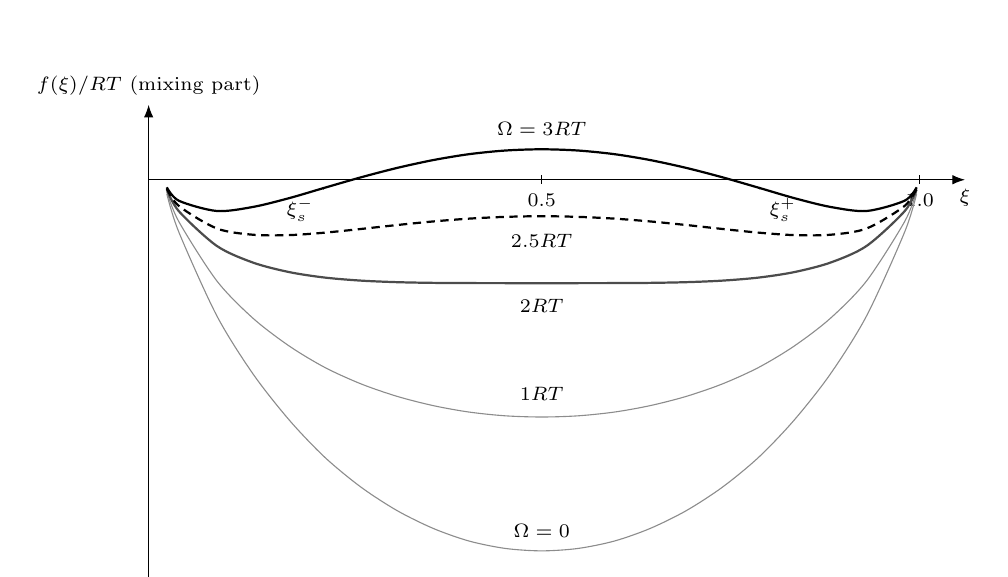
\begin{tikzpicture}[x=9.6cm,y=6.8cm]
\draw[-{Latex[length=1.6mm]}] (-0.02,-0.76) -- (-0.02,0.14) node[above,font=\scriptsize] {$f(\xi)/RT$ (mixing part)};
\draw[-{Latex[length=1.6mm]}] (-0.02,0) -- (1.06,0) node[below,font=\scriptsize] {$\xi$};
\foreach \xx in {0.5,1.0} {\draw (\xx,0.008) -- (\xx,-0.008) node[below,font=\scriptsize] {\xx};}
% Omega = 0 RT (ideal mixing)
\draw[black!45] plot[smooth] coordinates {(0.004,-0.0261) (0.020,-0.0980) (0.070,-0.2536) (0.118,-0.3625) (0.166,-0.4488) (0.213,-0.5183) (0.261,-0.5742) (0.309,-0.6182) (0.357,-0.6515) (0.404,-0.6748) (0.452,-0.6886) (0.500,-0.6931) (0.548,-0.6886) (0.596,-0.6748) (0.643,-0.6515) (0.691,-0.6182) (0.739,-0.5742) (0.787,-0.5183) (0.834,-0.4488) (0.882,-0.3625) (0.930,-0.2536) (0.980,-0.0980) (0.996,-0.0261)};
% Omega = 1 RT
\draw[black!45] plot[smooth] coordinates {(0.004,-0.0221) (0.020,-0.0784) (0.070,-0.1885) (0.118,-0.2586) (0.166,-0.3106) (0.213,-0.3505) (0.261,-0.3813) (0.309,-0.4047) (0.357,-0.4220) (0.404,-0.4339) (0.452,-0.4409) (0.500,-0.4431) (0.548,-0.4409) (0.596,-0.4339) (0.643,-0.4220) (0.691,-0.4047) (0.739,-0.3813) (0.787,-0.3505) (0.834,-0.3106) (0.882,-0.2586) (0.930,-0.1885) (0.980,-0.0784) (0.996,-0.0221)};
% Omega = 2 RT (threshold: flat bottom)
\draw[thick,black!70] plot[smooth] coordinates {(0.004,-0.0181) (0.020,-0.0588) (0.070,-0.1234) (0.118,-0.1547) (0.166,-0.1725) (0.213,-0.1827) (0.261,-0.1884) (0.309,-0.1913) (0.357,-0.1926) (0.404,-0.1930) (0.452,-0.1931) (0.500,-0.1931) (0.548,-0.1931) (0.596,-0.1930) (0.643,-0.1926) (0.691,-0.1913) (0.739,-0.1884) (0.787,-0.1827) (0.834,-0.1725) (0.882,-0.1547) (0.930,-0.1234) (0.980,-0.0588) (0.996,-0.0181)};
% Omega = 2.5 RT (double well)
\draw[densely dashed,thick] plot[smooth] coordinates {(0.004,-0.0161) (0.020,-0.0490) (0.070,-0.0909) (0.118,-0.1027) (0.166,-0.1034) (0.213,-0.0988) (0.261,-0.0919) (0.309,-0.0845) (0.357,-0.0778) (0.404,-0.0726) (0.452,-0.0693) (0.500,-0.0681) (0.548,-0.0693) (0.596,-0.0726) (0.643,-0.0778) (0.691,-0.0845) (0.739,-0.0919) (0.787,-0.0988) (0.834,-0.1034) (0.882,-0.1027) (0.930,-0.0909) (0.980,-0.0490) (0.996,-0.0161)};
% Omega = 3 RT (double well, humped)
\draw[thick] plot[smooth] coordinates {(0.004,-0.0141) (0.020,-0.0392) (0.070,-0.0583) (0.118,-0.0508) (0.166,-0.0343) (0.213,-0.0149) (0.261,0.0046) (0.309,0.0222) (0.357,0.0369) (0.404,0.0478) (0.452,0.0546) (0.500,0.0569) (0.548,0.0546) (0.596,0.0478) (0.643,0.0369) (0.691,0.0222) (0.739,0.0046) (0.787,-0.0149) (0.834,-0.0343) (0.882,-0.0508) (0.930,-0.0583) (0.980,-0.0392) (0.996,-0.0141)};
% spinodal markers on Omega=3RT: xi_s = 0.2113 / 0.7887, f/RT = -0.0157
\fill (0.2113,-0.0157) circle (0.5pt) node[below left,font=\scriptsize] {$\xi_s^-$};
\fill (0.7887,-0.0157) circle (0.5pt) node[below right,font=\scriptsize] {$\xi_s^+$};
% curve labels at xi = 0.5 (each just off its own curve)
\node[font=\scriptsize] at (0.5,0.095) {$\Omega=3RT$};
\node[font=\scriptsize] at (0.5,-0.115) {$2.5RT$};
\node[font=\scriptsize] at (0.5,-0.235) {$2RT$};
\node[font=\scriptsize] at (0.5,-0.40) {$1RT$};
\node[font=\scriptsize] at (0.5,-0.655) {$\Omega=0$};
\end{tikzpicture}
\caption{정규용액 조성 자유에너지의 섞임 몫 $f(\xi)/RT=\xi\ln\xi+(1-\xi)\ln(1-\xi)+(\Omega/RT)\,\xi(1-\xi)$
(좌표는 식 그대로의 수치 평가). $\Omega\le2RT$ 면 한 웰, $\Omega=2RT$ 에서 바닥이 평탄해지고
(문턱, 식~\eqref{eq:sm-thresh}), $\Omega>2RT$ 면 가운데가 언덕이 된 이중웰 --- $\Omega=3RT$ 곡선의 점이
spinodal $\xi_s^\pm=0.2113/0.7887$ 이다. 닫힌 근은 \S\ref{sec:hys} 가 닫으며, 그 절의 이중웰 그림이 이 가족
중 $\Omega=3RT$ 한 장을 확대한 것이다.}
\label{fig:sm-gxi}
\end{figure}

\begin{figure}[t]
\centering
\begin{tikzpicture}[x=9.6cm,y=0.60cm]
\draw[-{Latex[length=1.6mm]}] (-0.02,0) -- (1.06,0) node[below,font=\scriptsize] {$\theta$};
\draw[-{Latex[length=1.6mm]}] (-0.02,-4.3) -- (-0.02,4.4)
  node[above,font=\scriptsize] {$(\mu-\mu^0)/RT$};
\foreach \xx in {0.25,0.5,0.75} {\draw (\xx,0.07) -- (\xx,-0.07) node[below,font=\scriptsize] {\xx};}
\foreach \yy in {-4,-2,2,4} {\draw (-0.014,\yy) -- (-0.026,\yy) node[left,font=\scriptsize] {\yy};}
% Omega/RT = 0
\draw[thin] plot[smooth] coordinates {(0.02,-3.892) (0.036,-3.288) (0.052,-2.903) (0.068,-2.618) (0.084,-2.389) (0.1,-2.197) (0.13,-1.901) (0.1689,-1.593) (0.2079,-1.338) (0.2468,-1.116) (0.2858,-0.9159) (0.3247,-0.7321) (0.3637,-0.5594) (0.4026,-0.3945) (0.4416,-0.2348) (0.4805,-0.07793) (0.5195,0.07793) (0.5584,0.2348) (0.5974,0.3945) (0.6363,0.5594) (0.6753,0.7321) (0.7142,0.9159) (0.7532,1.116) (0.7921,1.338) (0.8311,1.593) (0.87,1.901) (0.9,2.197) (0.916,2.389) (0.932,2.618) (0.948,2.903) (0.964,3.288) (0.98,3.892)};
% Omega/RT = 2 (threshold)
\draw[densely dashed] plot[smooth] coordinates {(0.02,-1.972) (0.036,-1.432) (0.052,-1.111) (0.068,-0.8898) (0.084,-0.7252) (0.1,-0.5972) (0.13,-0.421) (0.1689,-0.2689) (0.2079,-0.1692) (0.2468,-0.1029) (0.2858,-0.05908) (0.3247,-0.03103) (0.3637,-0.01415) (0.4026,-0.005038) (0.4416,-0.001072) (0.4805,-3.942e-05) (0.5195,3.942e-05) (0.5584,0.001072) (0.5974,0.005038) (0.6363,0.01415) (0.6753,0.03103) (0.7142,0.05908) (0.7532,0.1029) (0.7921,0.1692) (0.8311,0.2689) (0.87,0.421) (0.9,0.5972) (0.916,0.7252) (0.932,0.8898) (0.948,1.111) (0.964,1.432) (0.98,1.972)};
% Omega/RT = 4 (van der Waals loop)
\draw[thick] plot[smooth] coordinates {(0.02,-0.05182) (0.036,0.4244) (0.052,0.6809) (0.068,0.8382) (0.084,0.9388) (0.1,1.003) (0.13,1.059) (0.1689,1.055) (0.2079,0.9992) (0.2468,0.9097) (0.2858,0.7978) (0.3247,0.67) (0.3637,0.5311) (0.4026,0.3844) (0.4416,0.2326) (0.4805,0.07786) (0.5195,-0.07786) (0.5584,-0.2326) (0.5974,-0.3844) (0.6363,-0.5311) (0.6753,-0.67) (0.7142,-0.7978) (0.7532,-0.9097) (0.7921,-0.9992) (0.8311,-1.055) (0.87,-1.059) (0.9,-1.003) (0.916,-0.9388) (0.932,-0.8382) (0.948,-0.6809) (0.964,-0.4244) (0.98,0.05182)};
% extrema (= spinodal) on Omega/RT=4
\fill (0.1464,1.0657) circle (0.5pt) node[above,font=\scriptsize] {$\theta_s^-$};
\fill (0.8536,-1.0657) circle (0.5pt) node[below,font=\scriptsize] {$\theta_s^+$};
% curve labels
\node[font=\scriptsize] at (0.115,-3.05) {$\Omega=0$};
\node[font=\scriptsize,right] at (0.99,1.97) {$\Omega=2RT$};
\node[font=\scriptsize] at (0.10,1.75) {$\Omega=4RT$};
\end{tikzpicture}
\caption{격자기체 화학퍼텐셜 $(\mu(\theta)-\mu^0)/RT=\ln[\theta/(1-\theta)]+(\Omega/RT)(1-2\theta)$
의 개형(식~\eqref{eq:mu}; 좌표는 식 그대로의 수치 평가). $\Omega=0$ 단조(로그 몫이 양끝을
잠금), $\Omega=2RT$ 에서 중심 기울기 $0$(문턱, 식~\eqref{eq:sm-thresh}), $\Omega=4RT$ 는 비단조 --- 한
$\mu$ 에 세 $\theta$ 가 대응하는 van der Waals loop 이고 극값(점)이 spinodal $\theta_s^\pm=0.146/0.854$,
값 $\pm1.066$. \S\ref{sec:hys} 과주행 그림의 $V_\eq(\xi)$ 곡선은 이 곡선의 $\theta=1-\xi$·부호 반전
거울이라 같은 $\pm1.066$ 이 나타난다.}
\label{fig:sm-mu}
\end{figure}

\subsection{전기화학 연결 --- $\mu_\mathrm{Li}=\mu^0-sF(V-U)$ 와 평형 점유 logistic}\label{sec:sm-electro}
\textbf{(a) 출발 --- 전기화학 퍼텐셜과 삽입 반응.} 하전 종은 화학퍼텐셜에 정전 에너지가 더해진
\emph{전기화학 퍼텐셜}(electrochemical potential)로 평형을 판정한다:
\begin{equation}
\tilde\mu\;\equiv\;\mu+zF\phi
\label{eq:sm-emu}
\end{equation}
($z$ = 전하수, $\phi$ = 그 종이 있는 상의 정전 퍼텐셜). 삽입 반응
$\mathrm{Li}^++e^-+[\,]\rightleftharpoons\mathrm{Li}_{(\mathrm{host})}$ 의 평형은 양변 $\tilde\mu$ 합의 일치이고
(\S\ref{sec:center} 가 결과 사슬에서 같은 균형으로 진입한다), host 안의 Li 는 중성이라
$\tilde\mu_\mathrm{Li}=\mu_\mathrm{Li}$ 다:
\begin{equation}
\big(\mu_{\mathrm{Li}^+}+F\phi_S\big)+\big(\mu_{e^-}-F\phi_M\big)=\mu_\mathrm{Li}(\theta)
\label{eq:sm-workbal}
\end{equation}
($\phi_S$ = 전해질, $\phi_M$ = 작동 전극의 정전 퍼텐셜; $z_{\mathrm{Li}^+}{=}+1$, $z_{e^-}{=}-1$).

\textbf{(b) 연산 --- 기준전극으로 측정 전위를 결선.} 같은 전해질에 담긴 기준 Li 금속 전극도 자기 평형
$\mathrm{Li}^++e^-\rightleftharpoons\mathrm{Li}_{(\mathrm{metal})}$ 을 이룬다:
\begin{equation}
\big(\mu_{\mathrm{Li}^+}+F\phi_S\big)+\big(\mu_{e^-}-F\phi_\mathrm{ref}\big)=\mu_\mathrm{Li}^\mathrm{metal}.
\label{eq:sm-refbal}
\end{equation}
\eqref{eq:sm-workbal} 에서 \eqref{eq:sm-refbal} 을 빼면 전해질 몫($\mu_{\mathrm{Li}^+}+F\phi_S$)이
상쇄된다. 전자의 화학 몫도 상쇄되는데, 여기에는 한 단계가 숨어 있다 — 두 전극의 전자 화학퍼텐셜은
엄밀히는 재질에 따라 다르며, 그 차이(접촉 전위차)는 두 전극을 같은 재질의 도선 단자 사이에서 읽는 측정
전위의 조작적 정의에 흡수되어 별도 항으로 남지 않는다(전기화학의 표준 처리). 그 결과 측정 전위
$V\equiv\phi_M-\phi_\mathrm{ref}$(vs Li/Li$^+$)만 남는다:
\begin{equation}
\mu_\mathrm{Li}(\theta_\eq)-\mu_\mathrm{Li}^\mathrm{metal}=-F\,V.
\label{eq:sm-muV}
\end{equation}
전위를 올리면 host 안 Li 의 화학퍼텐셜이 정확히 $-FV$ 만큼 낮아진다 --- ``$V$ 를 올리면 탈리튬화''가 이 한 줄이다.

\textbf{(c) 중간식 --- 상수 덩이를 $U$ 로 묶기.} 식~\eqref{eq:sm-muV} 의 상수 $\mu_\mathrm{Li}^\mathrm{metal}$
를 전이 중심 $U\equiv(\mu_\mathrm{Li}^\mathrm{metal}-\mu^0)/F$ 로 재포장하면($s=+1$ --- \S\ref{sec:notation}
표의 유도 전용 고정 부호, 방향 부호 $\sigma_d$ 와 별개)
\begin{equation}
\mu_\mathrm{Li}(\theta_\eq)=\mu^0-sF\,(V-U),
\qquad
\Delta G_j\equiv\mu^0-\mu_\mathrm{Li}^\mathrm{metal}=-sF\,U_j
\label{eq:sm-eqcond}
\end{equation}
--- \S\ref{sec:center}(N2)가 결과 사슬에서 다시 세우는 평형 조건과 글자까지 같은 식이다($U_j>0
\Leftrightarrow\Delta G_j<0$, 곧 그 전이가 자발일 전위 창이 양수라는 부호 읽기도 동일). Chapter 2 의 식
(eq:muV)도 같은 관계다.

\textbf{(d) 박스 --- 평형 점유 logistic.} $\Omega_j=0$ 이면 \eqref{eq:sm-muideal} 를 \eqref{eq:sm-eqcond} 에
넣어 $RT\ln[\theta_\eq/(1-\theta_\eq)]=-sF(V-U)$, 로그를 풀면 닫힌 꼴이 나온다:
\begin{equation}
\boxed{\;\theta_\eq(V,T)=\frac{1}{1+e^{+sF(V-U)/RT}},\qquad
\xi_\eq(V,T)=1-\theta_\eq=\frac{1}{1+e^{-sF(V-U)/RT}},\qquad
w\equiv\frac{RT}{F}\;.}
\label{eq:sm-logistic}
\end{equation}
자리당 언어와의 일치 검산 --- 식~\eqref{eq:fermifn} 의 지수는 $\beta\,\Delta\mu$ 이고, 몰로 올리면
$(\mu^0-\mu_\mathrm{Li})/RT$, 여기에 \eqref{eq:sm-eqcond} 를 넣으면 $+sF(V-U)/RT$ --- 정확히
\eqref{eq:sm-logistic} 의 $\theta_\eq$ 지수다(자리당 쌍 $(k_BT,\,e)$ 가 몰당 $(RT,\,F)$ 로 한꺼번에 환산).
점유 $\theta_\eq$ 는 $V$ 에 감소하고 탈리튬화 진행률 $\xi_\eq$ 는 증가하는 logistic 이며,
그림~\ref{fig:sm-occ} 가 온도별 개형과 두 곡선의 여집합 교차를 보인다. 여기서 세 가지가 본론으로 이어진다.
\begin{enumerate}[label=(\roman*),leftmargin=2.2em,itemsep=1pt]
\item \textbf{일반화는 \S\ref{sec:width} 소관.} 고정 부호 $s$ 자리에 방향 부호 $\sigma_d$, 중심에 분기 중심
$U_j^{\,d}$(\S\ref{sec:hys}), 폭에 다중도 $w_j=n_jRT/F$ 를 넣은 것이 모델의 평형 진행률 $\xi_\eq$ 다 --- 단 지수의
$\sigma_d$ 는 $\mathrm{logistic}[-x]=1-\mathrm{logistic}[x]$ 에 의한 $\xi\leftrightarrow1-\xi$ 여집합
relabel 일 뿐 종 $\xi(1-\xi)$ 은 불변이라, 물리 작용처(\S\ref{sec:notation} 의 분극$\cdot$분기$\cdot$꼬리)로는
세지 않는다.
\item \textbf{동역학 경로와의 합류.} 같은 logistic 이 Eyring 속도식의 정지점(detailed balance,
\S\ref{sec:width})에서도 나온다 --- 평형비 $\xi_\eq/(1-\xi_\eq)=e^{sF(V-U)/RT}$ 가 두 경로에서 같으니,
통계(이 절)와 동역학(\S\ref{sec:width})은 한 분포의 두 유도다(\S\ref{sec:dist} 의 명제를 Part 0 이 평형
쪽에서 선결).
\item \textbf{$\Omega_j\ne0$ 이면 닫힌 logistic 이 아니다.} \eqref{eq:sm-eqcond} 에 상호작용까지 든
식~\eqref{eq:mu} 를 넣고 $\xi$ 좌표의 우함수 대칭(\S\ref{sec:sm-mf})을 쓰면
$RT\ln[\xi/(1-\xi)]+\Omega_j(1-2\xi)=sF(V-U)$ 의 암시적 등온선이 되고(\S\ref{sec:hys} 의 $V_\eq(\xi)$),
$\Omega_j>2RT$(식~\eqref{eq:sm-thresh})면 비단조다. 곧 닫힌 logistic 은 $\Omega_j=0$ 에서만 엄밀하며,
$\Omega_j\ne0$ 전이에 같은 서식을 계속 쓰는 것의 지위(평형 예측 vs 현상학적 폭)는 \S\ref{sec:width} 의
폭 이중지위가 가른다.
\end{enumerate}

\begin{signbox}
\textbf{부호(Part 0).} $s=+1$: $V\!\uparrow\Rightarrow\mu_\mathrm{Li}\!\downarrow$(식~\eqref{eq:sm-eqcond})
$\Rightarrow\theta_\eq\!\downarrow,\ \xi_\eq\!\uparrow$ --- 전위를 올리면 탈리튬화가 진행한다(본론 규약 일치).
$V=U\Rightarrow\theta_\eq=\xi_\eq=\tfrac12$, $T\to0$ 계단($w\to0$)·$T\!\uparrow$ 폭 비례($w=RT/F$).
방향 부호 $\sigma_d$ 의 작용처(분극$\cdot$분기$\cdot$꼬리)는 \S\ref{sec:notation}·\S\ref{sec:signcheck} 소관 --- Part 0 은 $s=+1$ 고정.
\end{signbox}

\begin{figure}[t]
\centering
\resizebox{\textwidth}{!}{%
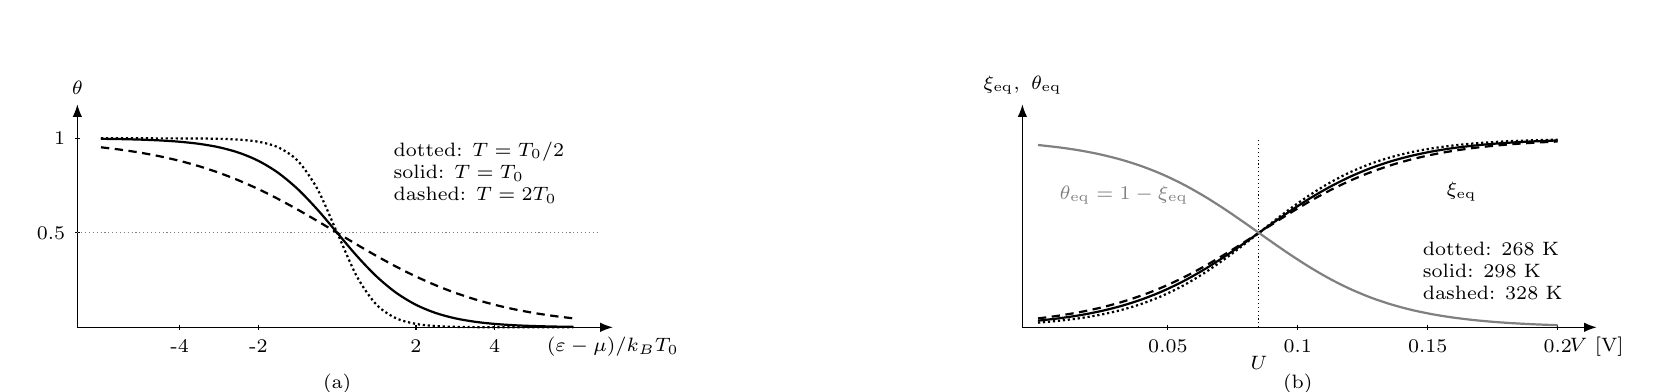
\begin{tikzpicture}
\begin{scope}[x=0.50cm,y=2.4cm]
% ---- (a) dimensionless single-site occupancy ----
\draw[-{Latex[length=1.6mm]}] (-6.6,0) -- (7.0,0)
  node[below,font=\scriptsize] {$(\varepsilon-\mu)/k_BT_0$};
\draw[-{Latex[length=1.6mm]}] (-6.6,0) -- (-6.6,1.18) node[above,font=\scriptsize] {$\theta$};
\foreach \xx in {-4,-2,2,4} {\draw (\xx,0.013) -- (\xx,-0.013) node[below,font=\scriptsize] {\xx};}
\draw (-6.54,1.0) -- (-6.66,1.0) node[left,font=\scriptsize] {1};
\draw (-6.54,0.5) -- (-6.66,0.5) node[left,font=\scriptsize] {0.5};
\draw[densely dotted,gray] (-6.6,0.5) -- (6.6,0.5);
% T = T0/2
\draw[thick,densely dotted] plot[smooth] coordinates {(-6,1) (-5,1) (-4,0.9997) (-3.5,0.9991) (-3,0.9975) (-2.5,0.9933) (-2,0.982) (-1.5,0.9526) (-1,0.8808) (-0.5,0.7311) (0,0.5) (0.5,0.2689) (1,0.1192) (1.5,0.04743) (2,0.01799) (2.5,0.006693) (3,0.002473) (3.5,0.0009111) (4,0.0003354) (5,4.54e-05) (6,6.144e-06)};
% T = T0
\draw[thick] plot[smooth] coordinates {(-6,0.9975) (-5.5,0.9959) (-5,0.9933) (-4.5,0.989) (-4,0.982) (-3.5,0.9707) (-3,0.9526) (-2.5,0.9241) (-2,0.8808) (-1.5,0.8176) (-1,0.7311) (-0.5,0.6225) (0,0.5) (0.5,0.3775) (1,0.2689) (1.5,0.1824) (2,0.1192) (2.5,0.07586) (3,0.04743) (3.5,0.02931) (4,0.01799) (4.5,0.01099) (5,0.006693) (5.5,0.00407) (6,0.002473)};
% T = 2T0
\draw[thick,densely dashed] plot[smooth] coordinates {(-6,0.9526) (-5.5,0.9399) (-5,0.9241) (-4.5,0.9047) (-4,0.8808) (-3.5,0.852) (-3,0.8176) (-2.5,0.7773) (-2,0.7311) (-1.5,0.6792) (-1,0.6225) (-0.5,0.5622) (0,0.5) (0.5,0.4378) (1,0.3775) (1.5,0.3208) (2,0.2689) (2.5,0.2227) (3,0.1824) (3.5,0.148) (4,0.1192) (4.5,0.09535) (5,0.07586) (5.5,0.06009) (6,0.04743)};
\node[font=\scriptsize,align=left] at (3.6,0.82)
  {dotted: $T=T_0/2$\\ solid: $T=T_0$\\ dashed: $T=2T_0$};
\node[font=\scriptsize] at (0,-0.30) {(a)};
\end{scope}
\begin{scope}[xshift=8.9cm,x=33cm,y=2.4cm]
% ---- (b) electrochemical dress: xi_eq(V), theta_eq(V) ----
\draw[-{Latex[length=1.6mm]}] (-0.006,0) -- (0.215,0) node[below,font=\scriptsize] {$V$ [V]};
\draw[-{Latex[length=1.6mm]}] (-0.006,0) -- (-0.006,1.18)
  node[above,font=\scriptsize] {$\xi_\eq,\ \theta_\eq$};
\foreach \xx in {0.05,0.1,0.15,0.2}
  {\draw (\xx,0.013) -- (\xx,-0.013) node[below,font=\scriptsize] {\xx};}
\draw[densely dotted] (0.085,0) -- (0.085,1.0);
\node[below,font=\scriptsize] at (0.085,-0.10) {$U$};
% xi_eq, T=268.15 K
\draw[thick,densely dotted] plot[smooth] coordinates {(0,0.02464) (0.008,0.03448) (0.016,0.04806) (0.024,0.06662) (0.032,0.09165) (0.04,0.1248) (0.048,0.1678) (0.056,0.2218) (0.064,0.2872) (0.072,0.3629) (0.08,0.4461) (0.088,0.5324) (0.096,0.6168) (0.104,0.6947) (0.112,0.7629) (0.12,0.8198) (0.128,0.8654) (0.136,0.9009) (0.144,0.9278) (0.152,0.9478) (0.16,0.9625) (0.168,0.9732) (0.176,0.9809) (0.184,0.9864) (0.192,0.9903) (0.2,0.9932)};
% xi_eq, T=298.15 K
\draw[thick] plot[smooth] coordinates {(0,0.03529) (0.008,0.04756) (0.016,0.06383) (0.024,0.08516) (0.032,0.1128) (0.04,0.1479) (0.048,0.1915) (0.056,0.2444) (0.064,0.3063) (0.072,0.3761) (0.08,0.4515) (0.088,0.5292) (0.096,0.6054) (0.104,0.6769) (0.112,0.7409) (0.12,0.7961) (0.128,0.8421) (0.136,0.8792) (0.144,0.9086) (0.152,0.9314) (0.16,0.9488) (0.168,0.962) (0.176,0.9719) (0.184,0.9792) (0.192,0.9847) (0.2,0.9887)};
% xi_eq, T=328.15 K
\draw[thick,densely dashed] plot[smooth] coordinates {(0,0.04716) (0.008,0.06163) (0.016,0.08017) (0.024,0.1037) (0.032,0.133) (0.04,0.1692) (0.048,0.2127) (0.056,0.2639) (0.064,0.3224) (0.072,0.3871) (0.08,0.4559) (0.088,0.5265) (0.096,0.596) (0.104,0.6619) (0.112,0.7221) (0.12,0.7752) (0.128,0.8206) (0.136,0.8586) (0.144,0.8896) (0.152,0.9145) (0.16,0.9342) (0.168,0.9496) (0.176,0.9615) (0.184,0.9707) (0.192,0.9778) (0.2,0.9832)};
% theta_eq = 1 - xi_eq, T=298.15 K
\draw[gray,thick] plot[smooth] coordinates {(0,0.9647) (0.008,0.9524) (0.016,0.9362) (0.024,0.9148) (0.032,0.8872) (0.04,0.8521) (0.048,0.8085) (0.056,0.7556) (0.064,0.6937) (0.072,0.6239) (0.08,0.5485) (0.088,0.4708) (0.096,0.3946) (0.104,0.3231) (0.112,0.2591) (0.12,0.2039) (0.128,0.1579) (0.136,0.1208) (0.144,0.09142) (0.152,0.06864) (0.16,0.05122) (0.168,0.03803) (0.176,0.02814) (0.184,0.02077) (0.192,0.0153) (0.2,0.01125)};
\node[font=\scriptsize] at (0.163,0.72) {$\xi_\eq$};
\node[gray,font=\scriptsize] at (0.033,0.70) {$\theta_\eq=1-\xi_\eq$};
\node[font=\scriptsize,align=left] at (0.175,0.30)
  {dotted: 268 K\\ solid: 298 K\\ dashed: 328 K};
\node[font=\scriptsize] at (0.1,-0.30) {(b)};
\end{scope}
\end{tikzpicture}%
}
\caption{단일 자리 점유의 전기화학적 재매개변수화(좌표는 식 그대로의 수치 평가). (a) 식~\eqref{eq:fermifn} 의
$\theta$ --- $\varepsilon=\mu$ 에서 $\tfrac12$, 낮은 $T$ 일수록 계단($\beta\to\infty$ --- $T\to0$ 극한이
계단 함수다), 높은 $T$ 일수록 완만. (b) 식~\eqref{eq:sm-logistic} 의 $\xi_\eq(V)$ ($U=0.085$ V, stage
$2\!\to\!1$ 초기값) --- 폭 $w=RT/F$ 가 $23.1/25.7/28.3$ mV($268/298/328$ K)로 $T$ 에 비례해 열리고, 회색
$\theta_\eq=1-\xi_\eq$ 와 중심 $V=U$ 에서 교차한다($\tfrac12$).}
\label{fig:sm-occ}
\end{figure}

\subsection{거시 열역학으로 --- $G\equiv H-TS$, $\Delta G_j=-sFU_j$, Nernst 식}\label{sec:sm-macro}
\textbf{(a) 출발 --- 두 언어의 같은 $\mu$.} 본론 \S\ref{sec:center} 는 거시 정의 --- Gibbs 자유에너지
$G\equiv H-TS$ 와 $\mu\equiv\partial G/\partial n|_{T,P}$ --- 에서 출발한다. 통계역학 쪽 정의는
\S\ref{sec:sm-ensemble} 의 $\mu=\partial F/\partial N|_{T,V}$ 였다. 둘의 다리는 $G=F+PV$ 다 --- 응축상
격자에 이온 1몰을 넣을 때의 $P\Delta v$ 몫은 $RT$·전기 일($FV$) 스케일에 비해 무시되므로
\begin{equation}
\mu=\frac{\partial G}{\partial n}\Big|_{T,P}\;\simeq\;\frac{\partial F}{\partial n}\Big|_{T,V}
\qquad(\text{삽입 고체: }P\Delta v\ll RT,\;F\,V)
\label{eq:sm-mubridge}
\end{equation}
--- \S\ref{sec:sm-lattice}--\S\ref{sec:sm-electro} 에서 세운 $\mu(\theta)$ 를 본론의 거시 $\mu$ 자리에
그대로 꽂아도 되는 근거가 이 한 줄이다.

\textbf{(b) 연산 --- 반응 자유에너지의 $H,S$ 분해.} \eqref{eq:sm-eqcond} 의 비배치 몫
$\Delta G_j=\mu^0-\mu_\mathrm{Li}^\mathrm{metal}$ 은 온도의 함수이고, $G\equiv H-TS$ 를 반응 차분에 적용하면
$\Delta G_j(T)=\Delta H_{\rxn,j}-T\Delta S_{\rxn,j}$ 다. \textbf{(c) 중간식 --- 평형 중심의 온도 환산.}
이를 $\Delta G_j=-sFU_j$ 와 등치하면 $\Delta H_{\rxn,j}-T\Delta S_{\rxn,j}=-FU_j(T)$($s{=}1$) --- 그 이항이
\S\ref{sec:center} 의 결과 박스($U_j(T)$·$\partial U_j/\partial T=\Delta S_{\rxn,j}/F$)이며, 박스는 그 절의
것을 그대로 쓰고 여기 다시 적지 않는다.

\textbf{(d) 박스 --- Nernst 식으로 마감.} 마지막으로 \eqref{eq:sm-logistic} 의 $\xi_\eq$ 를 전위에 대해
뒤집으면($\xi/(1-\xi)=e^{sF(V-U)/RT}$ 의 로그) 이상 극한($\Omega_j=0$)의 평형 전위 곡선이 닫힌다:
\begin{equation}
\boxed{\;
\Delta G_j=-sF\,U_j,
\qquad
V_\eq(\xi)=U_j+\frac{RT}{sF}\,\ln\frac{\xi}{1-\xi}
\qquad(\Omega_j=0,\ s=+1)\;.}
\label{eq:sm-nernst}
\end{equation}
로그 몫의 정체는 \eqref{eq:sm-Smix} 섞임 엔트로피의 부분몰 몫이다 --- Nernst 식의 $\ln[\xi/(1-\xi)]$ 는
곡선맞춤이 아니라 배치 셈법에서 온다(Chapter 2 의 식 (eq:Vxi)가 같은 결론을 발열 관점에서 재사용한다).
극한·부호 검산 --- $\xi=\tfrac12$ 에서 $V=U_j$(중심), $T\!\uparrow$ 이면 로그 몫의 기울기(폭 $w=RT/F$)가
비례해 커지고, $\Delta S_{\rxn,j}>0$ 이면 중심이 온도에 오른다. 상호작용 몫 $\Omega_j(1-2\xi)/sF$ 를 더하면
\S\ref{sec:hys} 의 $V_\eq(\xi)$ 로 확장되고, $\Omega_j>2RT$ 의 비단조가 히스테리시스로 이어진다.

\begin{keybox}
\textbf{Part 0 사다리.} 등확률~\eqref{eq:sm-S} $\to$ Gibbs 인자·$\Xi$~\eqref{eq:sm-gc} $\to$ 단일 자리
$\theta$~\eqref{eq:fermifn}·요동~\eqref{eq:sm-flucres} $\to$ lattice gas·섞임 엔트로피~\eqref{eq:sm-Smix}
$\to$ 평균장 $\Omega$~\eqref{eq:mu}·\eqref{eq:gxi}·문턱~\eqref{eq:sm-thresh} $\to$ 전위
손잡이~\eqref{eq:sm-eqcond} $\to$ logistic~\eqref{eq:sm-logistic}·Nernst~\eqref{eq:sm-nernst}. 본론이 결과로
쓰는 평형식의 전 유도가 이 사다리에 있다 --- 이후 절은 같은 사다리를 결과 사슬(코드 진행 N1--N9) 순서로
다시 밟는다.
\end{keybox}

% ====================================================================
\section{분극 — 측정 전위에서 내부 전위로 (N1)}\label{sec:pol}
% ====================================================================
이 계산의 첫 식은 분극을 벗기는 환산이다. 관측은 유한 전류에서 이루어지므로 측정 전위 $V_\app$ 에는 셀의
직렬 저항을 통과한 IR 분극이 실려 있고, 평형 열역학이 사는 전위는 그 분극을 벗긴 내부 전위 $V_n$ 이다.

\subsection{분극 부호 — 방향이 결정한다}
\textbf{(a) 출발 — 측정 전위와 내부 전위의 차.} 전류 크기 $|I|$ 가 lumped 저항 $R_n$ 을 통과하며 만드는 전위 강하는
크기 $|I|R_n$ 이고, 그 부호는 전류 방향이 정한다. 측정 전위는 내부 전위에 분극이 더해진 값이므로 한 방향(방전)에서
\begin{equation}
V_\app\;=\;V_n+\sigma_d\,|I|\,R_n
\qquad(\sigma_d=+1\ \text{방전})
\label{eq:vapppol}
\end{equation}
로 적는다 — 방전($\sigma_d=+1$)은 음극에서 산화(탈리튬화)가 일어나는 방향이라 측정 전위가 내부 전위보다 분극만큼
\emph{높게} 관측된다($V_\app>V_n$). 충전($\sigma_d=-1$)은 부호가 반대다. \textbf{(b) 연산 — $V_n$ 으로 이항.}
식~\eqref{eq:vapppol} 을 $V_n$ 에 대해 풀면(분극 항을 좌변으로 옮겨)
\begin{equation}
V_n\;=\;V_\app-\sigma_d\,|I|\,R_n,
\label{eq:vnmid}
\end{equation}
\textbf{(c) 두 방향을 한 식으로.} $\sigma_d$ 가 두 방향을 모두 흡수하므로 식~\eqref{eq:vnmid} 가 곧 박스다:
\begin{equation}
\boxed{\;V_n\;=\;V_\app\;-\;\sigma_d\,|I|\,R_n\;.}
\label{eq:vn}
\end{equation}
부호 약속을 식으로 확인하면 —
방전에서 $V_n=V_\app-|I|R_n<V_\app$(측정이 내부보다 높음), 충전에서 $V_n=V_\app+|I|R_n>V_\app$ — 이며,
$|I|\to0$ 또는 $R_n=0$ 에서 $V_n=V_\app$ 로 두 전위가 일치한다.

\subsection{작업 격자 — 꼬리가 들어올 여유}
이후 모든 전이 계산은 $V_n$ 을 직접 쓰지 않고, $V_n$ 의 범위를 양쪽으로 넓힌 균일 \emph{작업 격자}(수치 grid — 결정 lattice 와 무관) $V_\work$ 위에서
이루어진다. 넓힘은 동역학 꼬리(\S\ref{sec:tail})가 격자 밖에서 잘려 인공 절단이 생기지 않도록 하는 여유다.
$v_\mathrm{lo}=\min V_n$, $v_\mathrm{hi}=\max V_n$, $\Delta v=v_\mathrm{hi}-v_\mathrm{lo}$ 로
\begin{equation}
V_\work=\mathrm{linspace}\big(v_\mathrm{lo}-p_\mathrm{lo}\,\Delta v,\;
v_\mathrm{hi}+p_\mathrm{hi}\,\Delta v,\;n_\work\big),
\qquad \Delta_\mathrm{grid}=V_{\work,1}-V_{\work,0},
\label{eq:vwork}
\end{equation}
패딩 $p_\mathrm{lo}=p_\mathrm{hi}=0.15$, 점 수 $n_\work=\max(2048,\,2\,\mathrm{len}(V_n))$ 이다. 스팬은 하한
$10^{-6}$ V 아래로 내려가지 않도록 고정된다(단일점$\cdot$스칼라 입력의 격자 퇴화 가드). 온도가 배열 $T(V)$ 이면 같은 격자 위로 보간해 $T_\work$ 를 얻고($T_\mathrm{rep}=\overline{T_\work}$ 는
전이당 상수 평가용 대표 온도), 스칼라면 $T_\work\equiv T$ 다. 배경은 작업 격자 위에서 먼저 깔린다:
$\dd Q/\dd V|_\work \leftarrow C_\bg(V_\work)$. 모든 전이 기여는 여기에 더해지고($\mathrm N9$), 마지막에 $V_n$ 으로
역보간된다.

\begin{keybox}
\textbf{세 전위.} $V_\app$(측정)$\cdot$$V_n$(내부, 식~\eqref{eq:vn})$\cdot$$V_\work$(계산 격자, 식~\eqref{eq:vwork})는
지위가 다르다. 다음 절부터 평형$\cdot$동역학은 $V_\work$ 위에서 풀고, 출력만 $V_n$ 으로 되돌린다.
\end{keybox}

다음 절은 전이 루프의 첫 식 — 평형 중심 $U_j(T)$ — 으로 들어간다. 그 식이 어디서 오는지를 보이려면 먼저 평형을
판정하는 자유에너지 언어가 필요하므로, 다음 절은 $G\to\mu\to$ 평형 조건으로 이어지는 관계식부터 세운다.

% ====================================================================
\section{평형 중심 $U_j(T)$ — 열역학에서 (N2)}\label{sec:center}
% ====================================================================
전이 루프 안의 첫 물리량은 전이 $j$ 의 평형 중심 전위 $U_j(T)$ 다. 이 값은 열역학 입력 $(\Delta H_\rxn,\Delta S_\rxn)$
에서 식~\eqref{eq:Uj}로 계산되거나, 주어지지 않으면 $U$ 값을 직접 취한다. 이 절은 그 환산식이 어디서 오는지를, Gibbs
자유에너지의 정의에서 한 단계씩 닫는다. 이 유도가 딛는 통계역학적 기원($Z\to\mu$·전기화학 결선·$G\simeq F$ 다리)은
Part 0(\S\ref{sec:sm-ensemble}$\cdot$\S\ref{sec:sm-electro}$\cdot$\S\ref{sec:sm-macro})가 세웠다 — 이 절은 그 위에서 코드 입력
$(\Delta H_\rxn,\Delta S_\rxn)$ 으로 잇는 결과 사슬 쪽이다.

\subsection{$G,\mu$ 와 평형 조건 — 유도}
\textbf{(a) 출발 — 두 정의.} 등온$\cdot$등압 계(전지)의 자발성$\cdot$평형을 판정하는 퍼텐셜은 Gibbs 자유에너지
\begin{equation}
G\;\equiv\;H-TS
\label{eq:gibbsdef}
\end{equation}
이고($H$ 항과 $-TS$ 항의 상대적 크기를 온도가 정한다), 입자 1몰 변화당 $G$ 변화가 화학퍼텐셜이다:
\begin{equation}
\mu\;\equiv\;\frac{\partial G}{\partial n}\Big|_{T,P}.
\label{eq:mudef}
\end{equation}
두 장소의 $\mu$ 일치가 입자 교환 평형이다. \textbf{(b) 연산 — 삽입 반응의 전기화학 평형.} 리튬은 Li$^+$ 와 $e^-$ 로
갈라져 드나들므로 각 종의 화학퍼텐셜에 전기 일 $zF\phi$(1몰)가 더해진 전기화학 퍼텐셜 $\tilde\mu\equiv\mu+zF\phi$(식~\eqref{eq:sm-emu})가 균형을
이룬다. 삽입 반응 $\mathrm{Li}^++e^-+[\,]\rightleftharpoons\mathrm{Li}_{(\text{흑연})}$ 의 평형 조건
$\delta G=[\tilde\mu_\mathrm{Li}-\tilde\mu_{\mathrm{Li}^+}-\tilde\mu_{e^-}]\,\dd n=0$, 곧
\begin{equation}
\tilde\mu_{\mathrm{Li}^+}+\tilde\mu_{e^-}=\tilde\mu_\mathrm{Li}
\label{eq:eqbalance}
\end{equation}
에서, 전자 항이 $z=-1$ 이라 측정 전위 $V$ 를 통해 $\tilde\mu_{e^-}=\mu_{e^-}^0-FV$ 로 들어온다. \textbf{(c) 중간식 —
상수 덩이를 중심으로 흡수.} 좌변에서 $-FV$ 만 전위 의존이고 나머지(Li$^+$ 활동도$\cdot$기준 퍼텐셜)는 주어진 $T$ 에서
상수이므로, 그 상수 덩이를 $sFU$ 로 정의해($s=+1$ 라 $-FV=-sFV$) 묶으면 평형 조건이
\begin{equation}
\mu_\mathrm{Li}(\theta_\eq)\;=\;\mu^0-sF\,(V-U),
\qquad \Delta G_j\;=\;-sF\,U_j
\label{eq:eqcond}
\end{equation}
형태가 된다($s$ 는 방전 규약 $+1$; $U$ 는 비배치 몫 자유에너지의 전위 환산). \textbf{(d) 부호 핵심.} $\Delta G_j=-sFU_j$ —
$U_j$ 가 양이면 $\Delta G_j<0$, 곧 전이가 자발 진행할 전위가 양의 중심이다. 또한 $V$ 상승(전자 화학퍼텐셜 하락)$\Rightarrow$
평형 점유율 하강, 곧 ``$V$ 를 올리면 탈리튬화''가 이 한 식에 이미 들어 있다(\S\ref{sec:width} 의 logistic 부호로 회수).

\subsection{$U_j(T)$ — 온도 환산}
\textbf{(a) 출발.} 평형 조건의 비배치 몫은 반응 자유에너지 $\Delta G_j=\Delta H_{\rxn,j}-T\Delta S_{\rxn,j}$ 다.
\textbf{(b) 연산 — 식~\eqref{eq:eqcond} 의 $\Delta G_j=-sFU_j$($s=+1$)에 대입.} \textbf{(c) 중간식 — $U_j$ 로 이항.}
\begin{equation}
\Delta H_{\rxn,j}-T\Delta S_{\rxn,j}=-F\,U_j
\quad\Longrightarrow\quad
U_j=-\frac{\Delta H_{\rxn,j}-T\Delta S_{\rxn,j}}{F}
\label{eq:Ujmid}
\end{equation}
\textbf{(d) 박스 — 분자 부호 정리.}
\begin{equation}
\boxed{\;U_j(T)\;=\;\frac{-\Delta H_{\rxn,j}+T\,\Delta S_{\rxn,j}}{F}\;.}
\label{eq:Uj}
\end{equation}
부호 — 발열 반응
$\Delta H_\rxn<0$ 이면 분자 $-\Delta H_\rxn>0$ 이 중심을 \emph{올린다}(흡열 아님에 주의). 온도 의존은 식~\eqref{eq:Uj} 를
$T$ 로 미분한 $\partial U_j/\partial T=\Delta S_{\rxn,j}/F$ 이고(Gibbs 항등식 $\partial\Delta G/\partial T=-\Delta S$ 와
식~\eqref{eq:eqcond} 의 $\Delta G=-FU$ 를 잇는 것과 같다), $|\Delta S_\rxn|\sim$ 수$\sim$수십 J/(mol\,K) 라 $30$ K
창에서 수 mV 규모로 중심이 이동한다 — 다온도 피팅에서 온도마다 $U_j(T)$ 를 따로 읽어야 하는 이유다. 온도가 배열
$T_\work(V)$(비등온)이면 $U_j$ 도 격자별 배열로 나온다.

전이 중심의 실제 산출 경로를 정리하면 — $U_j(T)$ 는 열역학 입력 $(\Delta H_\rxn,\Delta S_\rxn)$ 이 주어지면
식~\eqref{eq:Uj} 로 계산되고(비등온이면 배열 $T_\work$ 그대로), 주어지지 않으면 $U$ 값을 직접 취한다. 이때
반응 엔트로피 자리에는 전극별 유효값이 들어가는데, 흑연에서는 입력 그대로(항등)이고 LCO 에서는 전자
엔트로피 항이 더해진다(\S\ref{sec:lco-code}). 수치 예시로 stage $2\to1$ 의 초기값
$\Delta H_\rxn=-13000$ J/mol, $\Delta S_\rxn=-16$ J/(mol\,K)를 넣으면
$U(298)=(13000-298.15\times16)/96485\approx0.0853$ V 로 목표 $0.085$ V 와 정합한다. 구현 대응은
부록~\ref{sec:appendix-code} 에 둔다.

다음은 같은 루프 안에서 이 중심을 충$\cdot$방전으로 갈라놓는 히스테리시스 분기다 — 그 갈림은 식~\eqref{eq:mudef} 의
$\mu$ 에 상호작용 몫이 들어가 평형이 비틀리는 데서 온다.

% ====================================================================
\section{히스테리시스 분기 중심 (N3)}\label{sec:hys}
% ====================================================================
평형 중심 $U_j$ 는 상호작용 $\Omega_j$ 와 분기 인자 $\gamma_j$ 가 있으면 방향별 분기 중심 $U_j^{\,d}$ 로 이동한다
(그렇지 않으면 $U_j$ 그대로). 본 문건의 주 전개는 방전이며, 히스테리시스는 그 위의 \emph{구조적 분기}로 선언된다 — 방전과 충전이
같은 전이를 서로 다른 준안정 가지로 과주행해 중심이 갈라진다(삽입형 전극 히스테리시스의 열역학적 기원\cite{dreyer2010}).
이 절은 그 gap 의 닫힌 식과 부호를, 격자기체 자유에너지의
이중웰에서 spinodal 을 거쳐 단계적으로 유도한다.

\subsection{상호작용이 평형을 비트는 곳 — $\mu(\theta)$ 의 상호작용 몫}
\textbf{(a) 출발 --- Part 0 의 결과 받기.} 한 전이를 ``동등한 자리에 리튬이 차고 비는'' 격자기체로 보면,
점유율 $\theta$ 의 화학퍼텐셜과 진행률 좌표의 정규용액 자유에너지는 Part 0 이 세운
식~\eqref{eq:mu}$\cdot$\eqref{eq:gxi} 그대로다($\Omega_j>0$ 이면 동종 이웃 인력 --- 가운데를 위로 밀어
이중웰의 씨앗, 식~\eqref{eq:sm-thresh}). \textbf{(b) 연산 --- 두 번 미분.}
식~\eqref{eq:gxi} 를 두 번 $\xi$ 로 미분하면(로그 몫의 1계 미분 $RT\ln[\xi/(1-\xi)]$, 2계 미분
$RT/[\xi(1-\xi)]$; 상호작용 몫의 2계 미분 $-2\Omega$)
\begin{equation}
g_j''(\xi)=\frac{RT}{\xi(1-\xi)}-2\Omega_j.
\label{eq:gpp}
\end{equation}
\textbf{(c) spinodal — $g_j''=0$ 의 근.} $g_j''=0$ 은 $\xi(1-\xi)=RT/(2\Omega_j)$, 곧 $\xi^2-\xi+RT/(2\Omega_j)=0$
의 근의 공식으로
\begin{equation}
\xi_{s,j}^\pm=\tfrac12(1\pm u_j),\qquad
u_j\equiv\sqrt{1-\frac{2RT}{\Omega_j}}\quad(\Omega_j>2RT).
\label{eq:spinodal}
\end{equation}
$u_j$ 가 실수가 되는 조건 $\Omega_j>2RT$ 가 상분리(따라서 히스테리시스)의 문턱이며($g''<0$ 구간이 생겨 한 전위에 여러
$\xi$ — 그림~\ref{fig:doublewell}), $\Omega_j\le2RT$ 면 갈라짐이 없다. 이 문턱을 넘지 못하면($\Omega_j\le2RT$) 분기 gap 은 정확히 0 이다(식~\eqref{eq:dUhys} 참조).

\begin{figure}[t]
\centering
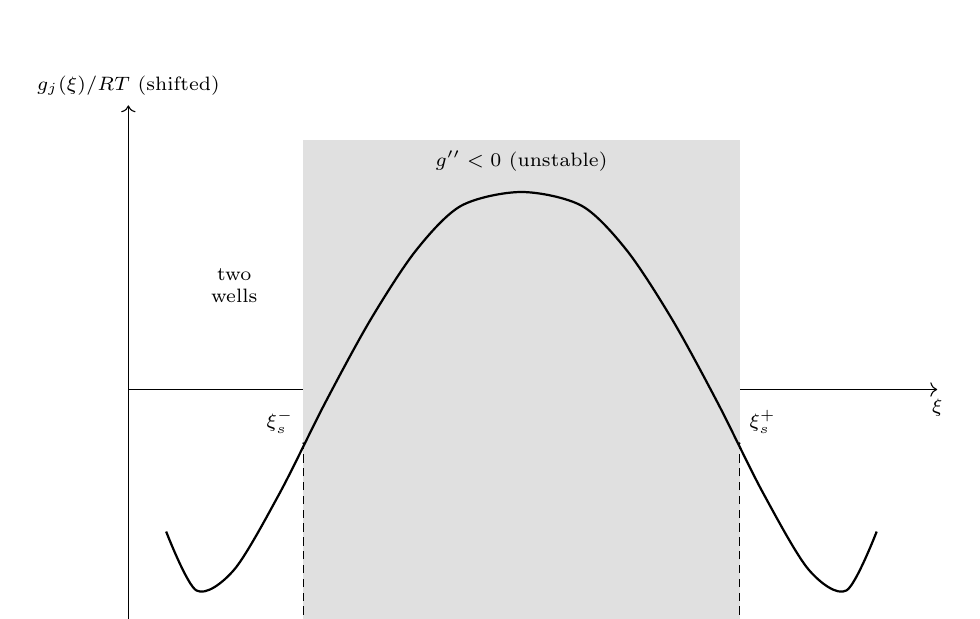
\begin{tikzpicture}[x=9.6cm,y=44cm]
% double-well free energy g(xi) for Omega=3RT (qualitative shape, normalized)
\draw[->] (-0.02,-0.069) -- (-0.02,0.082) node[above,font=\scriptsize] {$g_j(\xi)/RT$ (shifted)};
\draw[->] (-0.02,0) -- (1.05,0) node[below,font=\scriptsize] {$\xi$};
\foreach \xx in {0.25,0.5,0.75} {\draw (\xx,0.0015) -- (\xx,-0.0015) node[below,font=\scriptsize] {\xx};}
% spinodal band (g''<0) shading
\fill[black!12] (0.2113,-0.069) rectangle (0.7887,0.072);
\node[font=\scriptsize] at (0.5,0.066) {$g''<0$ (unstable)};
% the double well curve
\draw[thick] plot[smooth] coordinates {(0.03,-0.041) (0.07,-0.058) (0.12,-0.052) (0.18,-0.030) (0.24,-0.004) (0.3,0.020) (0.36,0.040) (0.42,0.053) (0.5,0.057) (0.58,0.053) (0.64,0.040) (0.7,0.020) (0.76,-0.004) (0.82,-0.030) (0.88,-0.052) (0.93,-0.058) (0.97,-0.041)};
% spinodal points
\fill (0.2113,-0.0155) circle (0.35pt) node[above left,font=\scriptsize] {$\xi_s^-$};
\fill (0.7887,-0.0155) circle (0.35pt) node[above right,font=\scriptsize] {$\xi_s^+$};
\draw[densely dashed] (0.2113,-0.069) -- (0.2113,-0.0155);
\draw[densely dashed] (0.7887,-0.069) -- (0.7887,-0.0155);
\node[font=\scriptsize,align=center] at (0.12,0.030) {two\\wells};
\end{tikzpicture}
\caption{격자기체 자유에너지 $g_j(\xi)$ (식~\eqref{eq:gxi} 의 \emph{개형}, $\Omega_j=3RT$ — 정성 곡선;
수치 정확 좌표는 그림~\ref{fig:sm-gxi} 의 같은 곡선). $\Omega>2RT$ 면 가운데가
언덕이 되어 양쪽에 골짜기 둘 — 음영 띠($g''<0$, 식~\eqref{eq:gpp})가 변곡점 $\xi_s^\pm$ (spinodal, 식~\eqref{eq:spinodal})
사이의 불안정 구간이다. 이 곡률 부호 전환이 \S\ref{sec:hys} 의 비단조 전위 곡선과 분기 gap 을 낳는다.}
\label{fig:doublewell}
\end{figure}

\subsection{gap 의 닫힌 꼴 — 두 spinodal 의 전위 차}
\textbf{(a) 출발 — 비단조 평형 전위 곡선.} 평형 조건~\eqref{eq:eqcond}($\mu=\mu^0-sF(V-U)$, 배치 몫 자유에너지 기울기 $=$ 전기화학 구동력)에 의해 자유에너지~\eqref{eq:gxi} 의 1계 미분이 곧 평형 전위에 묶인다
($g_j'(\xi)=RT\ln[\xi/(1-\xi)]+\Omega_j(1-2\xi)=sF(V_\eq-U_j)$). 1차(직선) 몫을 뗀 식~\eqref{eq:gxi} 가 \emph{1계} 미분에서도
옳은 근거는 Part 0 이 세운 조성 몫의 우함수 대칭(\S\ref{sec:sm-mf}: $f(1-\xi)=f(\xi)$, 따라서 $f'(1-\xi)=-f'(\xi)$)이다
— 식~\eqref{eq:mu} 의 $\mu_\mathrm{Li}(\theta)-\mu^0=f'(\theta)$
에 $\theta=1-\xi$ 를 넣으면 $\mu_\mathrm{Li}-\mu^0=f'(1-\xi)=-f'(\xi)=-g_j'(\xi)$ 가 되고, 뗀 선형 몫이 남긴 상수 $\mu^0$ 가
식~\eqref{eq:eqcond} 양변에서 상쇄돼 선형항 없이도 위 등식이 성립한다. 이를 $V_\eq$ 로 풀면
\begin{equation}
V_{\eq,j}(\xi)\;=\;U_j+\frac{RT}{sF}\ln\frac{\xi}{1-\xi}+\frac{\Omega_j}{sF}\,(1-2\xi),
\label{eq:Veq}
\end{equation}
이고 $\Omega_j>2RT$ 면 비단조다 — 방전은 $\xi\!\approx\!0$ 에서 상승 가지를 극대 $\xi_{s,j}^-$ 까지, 충전은 $\xi\!\approx\!1$
에서 극소 $\xi_{s,j}^+$ 까지 과주행하므로(전위 곡선의 극값이 $\dd V_\eq/\dd\xi=g_j''/sF=0$, 곧 spinodal 과 같은 점 —
그림~\ref{fig:hysloop}), 두 극값의 전위 차가 분기 gap 의 spinodal 상한이다. \textbf{(b) 연산 — spinodal 값 대입.}
식~\eqref{eq:spinodal} 의 $\xi_{s,j}^\pm=\tfrac12(1\pm u_j)$ 를 식~\eqref{eq:Veq} 의 두 비상수 항에 넣으면, logit 인자와
$(1-2\xi)$ 인자가 두 끝점에서 각각
\begin{equation}
\frac{\xi}{1-\xi}\bigg|_{\xi_{s,j}^\pm}=\frac{1\pm u_j}{1\mp u_j},
\qquad
(1-2\xi)\big|_{\xi_{s,j}^\pm}=\mp u_j
\label{eq:hyssub}
\end{equation}
— 곧 두 끝점에서 logit 인자가 서로 역수다. \textbf{(c) 중간식 — 극대에서 극소 빼기.} 극값 차를 적으면 상수항 $U_j$ 가
상쇄되고
\begin{align}
\Delta U_j^\hys
&=V_{\eq,j}(\xi_{s,j}^-)-V_{\eq,j}(\xi_{s,j}^+)\notag\\
&=\frac{RT}{sF}\Big[\ln\frac{1-u_j}{1+u_j}-\ln\frac{1+u_j}{1-u_j}\Big]
+\frac{\Omega_j}{sF}\big[u_j-(-u_j)\big]\notag\\
&=-\frac{4RT}{sF}\,\mathrm{artanh}\,u_j+\frac{2\Omega_j}{sF}\,u_j
\label{eq:hysdiff}
\end{align}
(둘째 줄의 두 로그가 부호 반대 같은 크기라 $\ln[(1-u)/(1+u)]-\ln[(1+u)/(1-u)]=-2\ln[(1+u)/(1-u)]=-4\,\mathrm{artanh}\,u$,
$\mathrm{artanh}\,u=\tfrac12\ln\tfrac{1+u}{1-u}$ 사용). \textbf{(d) 박스 — $s=+1$ 정리.}
\begin{equation}
\boxed{\;\Delta U_j^\hys
=\frac{2}{F}\Big[\Omega_j\,u_j-2RT\,\mathrm{artanh}\,u_j\Big],
\qquad u_j=\sqrt{1-\frac{2RT}{\Omega_j}}\;.}
\label{eq:dUhys}
\end{equation}
$\Omega_j\le2RT$ 면 gap 은
정확히 $0$ 이다(제곱근이 허수가 되는 영역의 명시 분기). 부호 — 극대 $>$ 극소라 $\Delta U_j^\hys\ge0$ 이고, $\Omega_j\to2RT^+$ 에서
$u_j\to0$ 이라 Taylor 전개($u_j$ 정의를 뒤집은 $\Omega_j=2RT/(1-u_j^2)$ 로
$\Omega_ju_j=2RT(u_j+u_j^3+\cdots)$, 그리고 $\mathrm{artanh}\,u=u+u^3/3+\cdots$ — 두 급수를 \emph{함께}
전개해야 하며, $\Omega_j\approx2RT$ 상수 대입만 하면 부호가 뒤집힌 $-\tfrac{4RT}{3F}u^3$ 에 이르는 함정이
있다)로 $\Delta U_j^\hys\to\frac{8RT}{3F}u_j^3\to0$ 으로
연속이다($u_j^3\propto(T_{c,j}-T)^{3/2}$, $T_{c,j}=\Omega_j/2R$ — 임계온도에서 매끄럽게 소멸).

\subsection{방향별 분기 중심 $U_j^{\,d}$}
\textbf{(a) 출발 — 두 spinodal 끝점의 평균.} 식~\eqref{eq:hyssub} 의 두 대입값으로 두 끝점의 \emph{평균}을 적으면
로그 몫 합 $\ln\frac{1-u}{1+u}+\ln\frac{1+u}{1-u}=0$ 과 $(1-2\xi)$ 몫 합 $u+(-u)=0$ 이 둘 다 $0$ 이라
\begin{equation}
\tfrac12\big[V_{\eq,j}(\xi_{s,j}^-)+V_{\eq,j}(\xi_{s,j}^+)\big]=U_j
\label{eq:hyssym}
\end{equation}
— 분기는 $U_j$ 대칭이다. \textbf{(b)(c) 한 자유도로.} 이 대칭 위에서 실측 분기 중심을 방향별 한 자유도로 적으면(축소
인자 $\gamma_j$ 와 부분 cycle 인자 $h_{\eta,j}$ 를 곱해)
\begin{equation}
\boxed{\;U_j^{\,d}\;=\;U_j\;+\;\tfrac12\,\sigma_d\,h_{\eta,j}\,\gamma_j\,\Delta U_j^\hys\;.}
\label{eq:Ubranch}
\end{equation}
\textbf{(d) 부호.} 방전($\sigma_d=+1$)은 중심을
$+$ 쪽, 충전($\sigma_d=-1$)은 $-$ 쪽으로 옮겨 $U_j^{\dis}>U_j^{\chg}$(방전 전위가 충전보다 높다는 관측 일치).
$\gamma_j=1$ 이 spinodal 상한, $\gamma_j\to0$ 이 히스 소멸, $h_{\eta,j}$ 가 부분 cycle 보정(기본 $1$)이다.

전이당 필요한 것은 상수인 분기 shift 뿐이므로, 식~\eqref{eq:Ubranch} 의 $U_j$ 자리에 $0$ 을 대입해 shift
분만 얻고, 배열 중심 $U_j$ 에 더한다:
\begin{equation}
\mathrm{center}=
\begin{cases}
U_j+\tfrac12\sigma_d h_{\eta,j}\gamma_j\Delta U_j^\hys(T_\rep) & \gamma_j\ne0 \text{ 이고 } \Omega_j>0\\[2pt]
U_j & \text{그 외(분기 없음)}.
\end{cases}
\label{eq:center}
\end{equation}
이 분기 중심(식~\eqref{eq:center})이 다음 절 평형 진행률 $\xi_\eq$ 의 중심으로 들어간다. 평형 종의 \emph{모양} 자체는 방향 불변이고,
방향이 바꾸는 것은 이 중심의 위치(와 \S\ref{sec:tail} 의 꼬리 방향)뿐이다.

\begin{figure}[t]
\centering
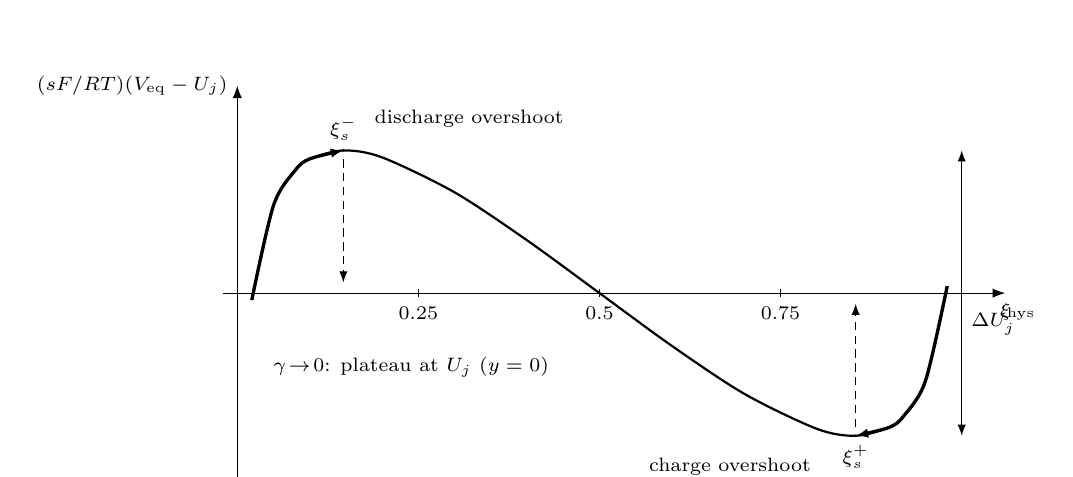
\begin{tikzpicture}[x=9.2cm,y=1.7cm]
\draw[-{Latex[length=1.6mm]}] (0,-1.45) -- (0,1.55) node[left,font=\scriptsize] {$(sF/RT)(V_\eq-U_j)$};
\draw[-{Latex[length=1.6mm]}] (-0.02,0) -- (1.06,0) node[below,font=\scriptsize] {$\xi$};
\foreach \xx in {0.25,0.5,0.75} {\draw (\xx,0.03) -- (\xx,-0.03) node[below,font=\scriptsize] {\xx};}
% non-monotone V_eq(xi) for Omega=4RT — exact 4dp: y = ln[xi/(1-xi)] + 4(1-2 xi)
\draw[thick] plot[smooth] coordinates {(0.02,-0.0518) (0.05,0.6556) (0.08,0.9177) (0.1,1.0028) (0.1464,1.0657) (0.2,1.0137) (0.3,0.7527) (0.4,0.3945) (0.5,0) (0.6,-0.3945) (0.7,-0.7527) (0.8,-1.0137) (0.8536,-1.0657) (0.9,-1.0028) (0.92,-0.9177) (0.95,-0.6556) (0.98,0.0518)};
\fill (0.1464,1.0657) circle (0.5pt) node[above,font=\scriptsize] {$\xi_s^-$};
\fill (0.8536,-1.0657) circle (0.5pt) node[below,font=\scriptsize] {$\xi_s^+$};
\draw[{Latex[length=1.4mm]}-{Latex[length=1.4mm]}] (1.0,-1.0657) -- (1.0,1.0657) node[pos=0.4,right,font=\scriptsize] {$\Delta U_j^\hys$};
% discharge overshoot path (rising branch up to xi_s^-)
\draw[-{Latex[length=1.6mm]},very thick] plot[smooth] coordinates {(0.02,-0.0518) (0.05,0.6556) (0.08,0.9177) (0.1,1.0028) (0.1464,1.0657)};
\draw[-{Latex[length=1.4mm]},densely dashed] (0.1464,1.0) -- (0.1464,0.08);
\node[font=\scriptsize] at (0.32,1.30) {discharge overshoot};
% charge overshoot path
\draw[-{Latex[length=1.6mm]},very thick] plot[smooth] coordinates {(0.98,0.0518) (0.95,-0.6556) (0.92,-0.9177) (0.9,-1.0028) (0.8536,-1.0657)};
\draw[-{Latex[length=1.4mm]},densely dashed] (0.8536,-1.0) -- (0.8536,-0.08);
\node[font=\scriptsize] at (0.68,-1.30) {charge overshoot};
\node[font=\scriptsize] at (0.24,-0.55) {$\gamma\!\to\!0$: plateau at $U_j$ ($y=0$)};
\end{tikzpicture}
\caption{비단조 평형 전위 $V_\eq(\xi)$(식~\eqref{eq:Veq}, $\Omega_j=4RT$ — 좌표는 식 그대로의 수치 평가)와 과주행. 방전(굵은 경로,
좌상)은 극대 $\xi_s^-$ 까지, 충전(우하)은 극소 $\xi_s^+$ 까지 과주행해 중심이 갈라진다. 두 극값 차가 spinodal 상한
gap $\Delta U_j^\hys$(식~\eqref{eq:dUhys}), 실측 분기는 $\gamma_j$ 만큼 안쪽(식~\eqref{eq:Ubranch}). $\gamma\to0$
가역 한계에서 두 경로가 $y=0$ plateau 로 합쳐진다.}
\label{fig:hysloop}
\end{figure}

% ====================================================================
\section{폭과 평형 진행률 $\xi_\eq$ (N4, N5)}\label{sec:width}
% ====================================================================
중심이 정해지면 다음으로 폭 $w_j$ 와 평형 진행률 $\xi_{\eq,j}$ 를 정한다. 이 둘이 평형 종(다음 절의 peak)의 모양을
결정한다. 평형 등온선은 \S\ref{sec:center} 의 평형 조건을 정$\cdot$역 속도의 균형으로 회수하면 logistic 으로 닫히는데,
그 회수가 이 절의 핵심 유도다 — 먼저 폭을 세운 뒤 logistic 을 detailed balance 에서 끌어낸다. 이 운동학 경로는 Part 0(\S\ref{sec:sm-electro})의 평형 통계
경로와 독립이며, 두 경로가 같은 logistic 에 닿는 것이 \S\ref{sec:dist} 의 통합이다.

\subsection{폭 $w_j$ — 이상 극한과 그 이중지위}
평형 진행률의 폭 척도는 이상 극한에서 $w_j=n_jRT/F$ 다($n_j$ 는 폭 다중도): 아래 소절 logistic 유도의
중심 기울기 $\dd\xi_\eq/\dd V|_{1/2}=sF/(4RT)$ 가 폭 척도 $RT/F$ 를 정의하고, 폭 다중도 $n_j$ 로 일반화하면
\begin{equation}
w_j=\frac{n_jRT}{F}\qquad(\text{기본 폭}),
\label{eq:wbase}
\end{equation}
폭이 직접 주어지면(대신 $w$ 값 자체가 입력되면) $n_j=w_jF/(RT)$ 로 역산해 같은 식에 넣는다.
폭은 항상 이 한 식을 쓴다(상호작용에 따라 폭을 인위로 좁히는 별도 항은 두지 않는다 — 그 까닭은 바로 아래
이중지위와 \S\ref{sec:broadening} 가 설명한다).

\textbf{★폭 $w_j$ 의 이중지위 — 같은 식, 다른 지위.} 식~\eqref{eq:wbase} 의 \emph{값}은 한 줄이지만, 그것이
\emph{무엇을 뜻하는지}는 전이의 상분리 여부로 갈린다. \emph{단상($\Omega_j\le2RT$, 연속 고용체)}에서는 $w_j=n_jRT/F$
가 등온선 폭에 대한 \emph{검증 가능한 평형 예측}이다 — 평형 단일 입자 dQ/dV 가 logistic
미분 종(\S\ref{sec:eqpeak} 에서 유도)이고, 그 폭이 곧 $n_jRT/F$ 라($n_j\!\approx\!1$ 이면 $RT/F\!\approx\!25.7$ mV), 측정 폭으로 직접 검증된다. 엄밀히 이 닫힌 폭은 이상 극한($\Omega_j=0$) 기준이고,
$0<\Omega_j<2RT$ 에서는 평형 등온선의 중심 기울기가 $(1-\Omega_j/2RT)$ 배 좁아진 유효 폭을 주되 그
값 역시 평형이 결정하므로 첫째 지위(평형 예측)라는 성격은 변하지 않는다(Chapter 2 파생 C 와 동일 취지).
\emph{두-상($\Omega_j>2RT$, 상분리 plateau)}에서는 평형이 예측하는 것이 폭이 아니라 \emph{날카로운 선}(델타)이므로,
같은 $w_j$ 가 더는 평형 예측이 아니라 \emph{broadening 이 정하는 현상학적 자유 피팅 폭}이다(\S\ref{sec:broadening}).
어느 지위인지는 인위적 구분이 아니라 그 전이의 \emph{$\Omega_j$ 값}이 가르며, 같은 식~\eqref{eq:wbase} 가 두 경우 모두에
쓰인다. 표~\ref{tab:staging} 의 흑연 staging 네 전이는 \emph{초기값} $\Omega_j$ 가 모두 $2RT(\!\approx\!4958$ J/mol
$@298$ K$)$ 보다 커 출발점에선 전부 둘째(두-상) 쪽에 놓이지만, 이 $\Omega_j$ 는 거친 초기 추정이라 피팅으로
override 되어 \emph{피팅 후} 물리적으로 전이별로 갈린다. dilute$\to$stage4 영역(피팅 전이 아님)과
4L$\to$3L$\cdot$3L$\to$2L 두 전이는
연속 고용체(solid-solution)라 후자 둘은 \emph{$\Omega_j<2RT$ 로 피팅되어 첫째 지위(평형 예측)}가 될 것으로 기대되고,
$2\mathrm L\!\to\!2$($\mathrm{LiC_{12}}$)$\cdot$$2\!\to\!1$($\mathrm{LiC_6}$) \emph{두 전이만} 두-상이라
\emph{$\Omega_j>2RT$ 를 유지해 둘째 지위(현상학적 폭)}로 남는다(전이별 구분은 \S\ref{sec:broadening}(a)).
곧 네 전이의 폭 출발값(0.020/0.016/0.014/0.012 V)도 같은 지위의 초기값이다($w$ 폴백 — $n_j$ 입력을
배제해야 활성화되며 현재 출발은 $n_j{=}1$: \S\ref{sec:broadening} ②) — 단상의 $w$ 는 평형이
정하고, 두-상의 $w$ 는 피팅이 정한다.

\subsection{평형 진행률 $\xi_\eq$ — logistic 의 유도}
\textbf{(a) 출발 — Eyring 속도식과 비대칭 장벽.} 활성화 장벽 $\Delta G_a$ 이상을 갖출 확률은 Boltzmann 분포
$\propto e^{-\Delta G_a/RT}$ 이고, 전이상태 이론의 시도 빈도 $k_0=k_BT/h$ 를 곱하면 Eyring 속도식
$k\simeq k_0e^{-\Delta G_a/RT}$ 다(그림~\ref{fig:barrier})\cite{eyring1935}. 구동력 $\mathcal A_j=sF(V_n-U_j)$ 가 정$\cdot$역 장벽을
비대칭 이동시켜(분율 위치 $\chi$ — 비평형 열역학 기반 전하전달 동역학의 표준 분해\cite{bazant2013}), 자리당 정$\cdot$역 속도가
\begin{equation}
r_j^+=k_0\,e^{-(\Delta G_{a,j}-\chi\mathcal A_j)/RT},\qquad
r_j^-=k_0\,e^{-(\Delta G_{a,j}+(1-\chi)\mathcal A_j)/RT}.
\label{eq:bv}
\end{equation}
\textbf{(b) 연산 — 비를 취해 detailed balance.} 두 속도의 비를 취하면 $k_0,e^{-\Delta G_a/RT}$ 가 약분되고 지수의
$\chi$ 가 상쇄되어($\chi\mathcal A+(1-\chi)\mathcal A=\mathcal A$)
\begin{equation}
\frac{r_j^+}{r_j^-}=\exp\!\Big[\frac{\chi\mathcal A_j+(1-\chi)\mathcal A_j}{RT}\Big]=\exp\!\Big[\frac{\mathcal A_j}{RT}\Big]
\label{eq:db}
\end{equation}
— 평형비가 $\chi$ 와 무관한 Boltzmann 비라는 detailed balance 다($\chi+(1-\chi)=1$ 합-1 제약이 강제한 결과). 운동
방정식은 정방향이 찬 자리($1-\xi$)에서, 역방향이 빈 자리($\xi$)에서 출발하므로
$\dd\xi/\dd t=r^+(1-\xi)-r^-\xi=k_j(\xi_\eq-\xi)$($k_j\equiv r^++r^-$). \textbf{(c) 중간식 — 정지점에서 logit.}
정지점 $\dd\xi/\dd t=0$ 에서 $r^+(1-\xi_\eq)=r^-\xi_\eq$(정$\cdot$역 플럭스의 교점 — 그림~\ref{fig:flux}), 곧
비 식~\eqref{eq:db} 로
\begin{equation}
\frac{\xi_\eq}{1-\xi_\eq}=e^{\mathcal A_j/RT}=e^{sF(V_n-U_j)/RT}
\quad\Longrightarrow\quad
\xi_\eq=\frac{1}{1+e^{-sF(V_n-U_j)/RT}}
\label{eq:logisticsolve}
\end{equation}
(둘째 식은 분모$\cdot$분자를 $e^{\mathcal A/RT}$ 로 나눈 것). \textbf{(d) 박스 — 폭 다중도$\cdot$방향 부호 일반화.}
폭 척도 $w_j=n_jRT/F$(식~\eqref{eq:wbase})로 묶고 방향 부호 $\sigma_d$ 와 분기 중심 $U_j^{\,d}$ 로 일반화하면
--- 충전의 진행률은 같은 분포의 여집합 좌표 $\theta=1-\xi$ 라 $s\to\sigma_d$ 치환은 여집합 교환과 동치다
(\S\ref{sec:dist}; 전극-중립 일반화는 \S\ref{sec:lco-direction}) ---
\begin{equation}
\boxed{\;\xi_{\eq,j}(V,T)=\frac{1}{1+\exp\!\big[-\sigma_d(V-U_j^{\,d})/w_j\big]}\;.}
\label{eq:xieq}
\end{equation}
열역학은 detailed balance~\eqref{eq:db} 한 곳으로만 들어왔다 — logistic 은 속도식의 정지점에서 \emph{유도된}
평형이다. 방향 부호가 logistic 인자의 부호로 들어가는 것이 식~\eqref{eq:xieq} 의
$z=\sigma_d(V-U_j^{\,d})/w_j$ 이며, 오버플로를 피하기 위해 $z\ge0/z<0$ 두 등가 형태로 나눠 평가한다(수학적으로
동일). 여기서 평가 전위는 내부 전위 $V_n$ 이 아니라 \S\ref{sec:pol} 의 작업 격자 $V_\work$ 다. 중심 $U_j^{\,d}$
는 식~\eqref{eq:center} 의 분기 중심(분기 있으면 분기 중심, 없으면 $U_j$)이다.

\begin{figure}[t]
\centering
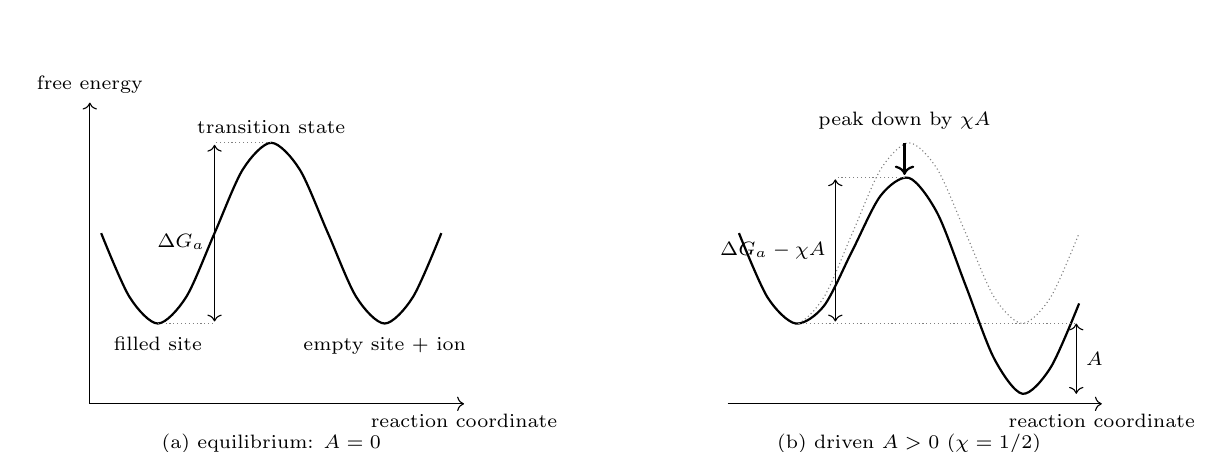
\begin{tikzpicture}[x=0.72cm,y=2.55cm]
% ---- (a) equilibrium landscape ----
\draw[->] (-0.2,-0.3) -- (6.4,-0.3) node[below,font=\scriptsize] {reaction coordinate};
\draw[->] (-0.2,-0.3) -- (-0.2,1.2) node[above,font=\scriptsize] {free energy};
\draw[thick] plot[smooth] coordinates {(0,0.55) (0.5,0.232) (1,0.1) (1.5,0.232) (2,0.55) (2.5,0.868) (3,1.0) (3.5,0.868) (4,0.55) (4.5,0.232) (5,0.1) (5.5,0.232) (6,0.55)};
\node[below,font=\scriptsize] at (1,0.08) {filled site};
\node[below,font=\scriptsize] at (5,0.08) {empty site + ion};
\node[above,font=\scriptsize] at (3,1.0) {transition state};
\draw[densely dotted,gray] (1,0.1) -- (2.0,0.1);
\draw[densely dotted,gray] (3,1.0) -- (2.0,1.0);
\draw[<->] (2.0,0.11) -- (2.0,0.99) node[pos=0.45,left,font=\scriptsize] {$\Delta G_a$};
\node[font=\scriptsize] at (3,-0.5) {(a) equilibrium: $A=0$};
\begin{scope}[xshift=8.1cm]
% ---- (b) driven landscape: A>0, chi=1/2 ----
\draw[->] (-0.2,-0.3) -- (6.4,-0.3) node[below,font=\scriptsize] {reaction coordinate};
\draw[densely dotted,thin,gray] plot[smooth] coordinates {(0,0.55) (0.5,0.232) (1,0.1) (1.5,0.232) (2,0.55) (2.5,0.868) (3,1.0) (3.5,0.868) (4,0.55) (4.5,0.232) (5,0.1) (5.5,0.232) (6,0.55)};
\draw[thick] plot[smooth] coordinates {(0,0.550) (0.5,0.232) (1,0.100) (1.5,0.188) (2,0.463) (2.5,0.737) (3,0.825) (3.5,0.649) (4,0.288) (4.5,-0.074) (5,-0.250) (5.5,-0.118) (6,0.200)};
\draw[->,thick] (2.92,1.0) -- (2.92,0.84) ;
\node[above,font=\scriptsize] at (2.92,1.02) {peak down by $\chi A$};
\draw[densely dotted,gray] (1.05,0.1) -- (1.7,0.1);
\draw[densely dotted,gray] (2.92,0.828) -- (1.7,0.828);
\draw[<->] (1.7,0.11) -- (1.7,0.818) node[pos=0.5,left,font=\scriptsize] {$\Delta G_a-\chi A$};
\draw[densely dotted,gray] (1.05,0.1) -- (5.95,0.1);
\draw[<->] (5.95,0.1) -- (5.95,-0.25) node[pos=0.5,right,font=\scriptsize] {$A$};
\node[font=\scriptsize] at (3,-0.5) {(b) driven $A>0$ ($\chi=1/2$)};
\end{scope}
\end{tikzpicture}
\caption{활성화 장벽 그림. (a) 평형 — 두 골짜기 같은 높이, 속도는 Eyring 식. (b) 구동력 $\mathcal A_j$ 가
도착 골짜기를 내리면 정방향 장벽 $\Delta G_a-\chi\mathcal A$, 역방향 $\Delta G_a+(1-\chi)\mathcal A$ 로 비대칭 이동
(식~\eqref{eq:bv}; 두 속도의 비가 식~\eqref{eq:db} detailed balance). 점선은 (a). 온도는 분모 $RT$ 로 진입.
이 그림이 식~\eqref{eq:xieq} logistic 과 \S\ref{sec:lag} 의 $L_q$ 두 결과의 공통 출발점이다.}
\label{fig:barrier}
\end{figure}

\begin{figure}[t]
\centering
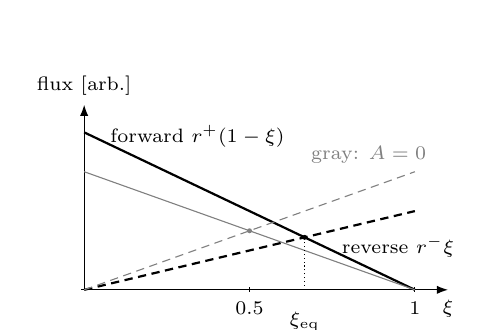
\begin{tikzpicture}[x=4.2cm,y=1.0cm]
\draw[-{Latex[length=1.4mm]}] (0,0) -- (0,2.35) node[above,font=\scriptsize] {flux [arb.]};
\draw[-{Latex[length=1.4mm]}] (-0.01,0) -- (1.1,0) node[below,font=\scriptsize] {$\xi$};
\foreach \xx in {0.5,1} {\draw (\xx,0.03) -- (\xx,-0.03) node[below,font=\scriptsize] {\xx};}
% forward r+ (1-xi): decreasing line from 2 to 0
\draw[thick] (0,2) -- (1,0);
% reverse r- xi: increasing line from 0 to 1
\draw[thick,densely dashed] (0,0) -- (1,1);
% A=0 pair (gray)
\draw[gray] (0,1.5) -- (1,0);
\draw[gray,densely dashed] (0,0) -- (1,1.5);
% intersection black: 2(1-xi)=xi -> xi=2/3
\draw[densely dotted] (0.6667,0) -- (0.6667,0.6667);
\fill (0.6667,0.6667) circle (0.9pt);
\node[below,font=\scriptsize] at (0.6667,-0.16) {$\xi_\eq$};
\fill[gray] (0.5,0.75) circle (0.9pt);
\node[right,font=\scriptsize] at (0.05,1.95) {forward $r^+(1-\xi)$};
\node[right,font=\scriptsize] at (0.75,0.55) {reverse $r^-\xi$};
\node[gray,font=\scriptsize] at (0.86,1.72) {gray: $A=0$};
\end{tikzpicture}
\caption{정지점 유도. 정방향 플럭스 $r^+(1-\xi)$(감소 직선)와 역방향 $r^-\xi$(증가 직선)의 교점이 정지점
$\xi_\eq$(식~\eqref{eq:logisticsolve}). $\mathcal A>0$($r^+=2r^-$, 검정)이면 $\xi_\eq=2/3$, $\mathcal A=0$
(회색)이면 $\tfrac12$ — detailed balance(식~\eqref{eq:db})가 평형을 정한다.}
\label{fig:flux}
\end{figure}

\begin{signbox}
\textbf{부호.} 방전 $\sigma_d=+1$: $V\!\uparrow\Rightarrow z\!\uparrow\Rightarrow\xi_\eq\!\uparrow$ — 전위를 올리면
탈리튬화 진행이 는다(규약 일치). 충전 $\sigma_d=-1$: $V\!\uparrow\Rightarrow z\!\downarrow\Rightarrow\xi_\eq\!\downarrow$.
극한 — $V\gg U_j^{\,d}\Rightarrow\xi_\eq\to1$(방전), $V\ll U_j^{\,d}\Rightarrow0$, $V=U_j^{\,d}\Rightarrow\tfrac12$
(전이 중심). $w_j=RT/F=25.7$ mV($25^\circ$C).
\end{signbox}

\subsection{같은 결과의 분포 관점 — $\xi_\eq$ 는 평형 점유 분포의 여집합}\label{sec:dist}
앞에서 $\xi_\eq$ 는 두 경로로 나왔다 — (i) kinetic: 속도식 정지점에서 detailed balance~\eqref{eq:db}(식~\eqref{eq:logisticsolve}),
(ii) thermo: 자유에너지 최소화 $g_j'(\xi)=sF(V_\eq-U)$(식~\eqref{eq:Veq}). 이 둘은 사실 \emph{하나의 분포}의 두 얼굴이다.
이 소절은 결과식$\cdot$부호$\cdot$코드는 그대로 두고 $\xi_\eq$ 의 통계역학적 정체만 밝혀,
\S\ref{sec:lco-electronic} 의 LCO 전자 엔트로피와 같은 언어로 두 곳을 묶는다.

\textbf{(a)(b) --- Part 0 회수.} 단일 자리 분포는 Part 0 이 이미 닫았다 --- grand-canonical
분배함수 $\Xi_1=1+e^{-\beta\Delta\mu}$(식~\eqref{eq:partfn}, 내부 자유도 $q(T)$ 흡수형)와 평균 점유
$\langle n\rangle=1/(1+e^{+\beta\Delta\mu})$(식~\eqref{eq:fermifn},
$\Delta\mu\equiv\tilde\varepsilon-\mu_\mathrm{Li}$)를 받는다. \textbf{(c) 같은 식 --- logistic 과의 일치.}
전기화학 구동력이 자리 점유 비용을 정한다 --- 전이 중심 기준(자리 자유에너지의 몰 환산 $N_A\tilde\varepsilon=\mu^0$)과
식~\eqref{eq:eqcond} 의 $\mu_\mathrm{Li}=\mu^0-sF(V-U)$ 를 정의에 넣으면 1몰 기준으로
$\Delta\mu=+sF(V-U_j)$, 곧 지수는 몰당 형태로
$\Delta\mu/(RT)=+s(V-U_j)/w_j$($w_j\equiv RT/F$, 이상 극한)다($\beta$ 의 자리당 $k_BT$ 가 몰당 $RT$ 로,
자리당 전하 $e$ 가 몰당 $F$ 로 한꺼번에 환산 --- 비는 불변). 따라서 식~\eqref{eq:fermifn} 은
$\langle n\rangle=1/(1+e^{+s(V-U_j)/w_j})=\theta_\eq$ --- $V$ 를 올리면 점유가 내려가는(탈리튬화) 자리 점유
그 자체이고, 본론의 진행률은 그 여집합 $\xi_\eq=1-\langle n\rangle=1/(1+e^{-s(V-U_j)/w_j})$ 로
식~\eqref{eq:logisticsolve}$\cdot$\eqref{eq:xieq} 와 일치한다(Chapter 2 의 식 (eq:logistic)과 부호까지 동일).
곧 \emph{$\xi_\eq$ 는 격자기체 평형 점유 확률 분포의 여집합}이며, 점유 $\theta_\eq$ 와 진행률 $\xi_\eq$ 를
가르는 한 번의 부호 차이는 방향 부호가 아니라 \emph{같은 분포를 읽는 두 좌표}(여집합 교환
$\xi=1-\theta$)의 차이다.

\textbf{(d) 두 경로의 통합.} kinetic(정$\cdot$역 플럭스 균형 점유, 식~\eqref{eq:db})$\cdot$thermo 두 경로
모두 \emph{같은 grand-canonical 평형 점유 분포}(식~\eqref{eq:fermifn})에 도달한다. $\Omega=0$(이상 격자기체)이면 분포가 정확히 Fermi-함수형이고, $\Omega>0$
이면 평균장 자리 비용 $\Delta\mu$ 에 $-\Omega(1-2\xi)$ 가 더해져(식~\eqref{eq:mu}) 자기무모순 분포가 된다 — 그
비단조성이 \S\ref{sec:hys} 의 히스이고, 그 분포가 접히는 점(자유에너지 $g$ 의 변곡, spinodal)이 식~\eqref{eq:spinodal} 이다. 곧 ``점유 분포''
한 언어가 평형 중심$\cdot$폭$\cdot$히스$\cdot$logistic 을 한 줄에 꿴다.

\begin{keybox}
\textbf{분포 다리.} $\xi_\eq$ 가 평형 점유 확률 분포(식~\eqref{eq:fermifn})라는 것이 \S\ref{sec:lco-electronic}
의 LCO \emph{전자} 엔트로피(전도 전자 Fermi--Dirac 분포 $f(E)=1/(1+e^{\beta(E-E_F)})$)와 \emph{동형}이다 —
흑연의 \emph{리튬 자리} 점유와 LCO 의 \emph{전자 준위} 점유가 같은 통계로 닫혀, 이 다리가 LCO 전자 엔트로피
절을 흑연 forward 틀 안으로 끌어들인다.
\end{keybox}

그림~\ref{fig:logistic} 가 $\xi_\eq$ 와 그 미분(다음 절의 종)을 함께 보이며, 다음 절은 이 종이 평형 peak 임을 닫는다.

\begin{figure}[t]
\centering
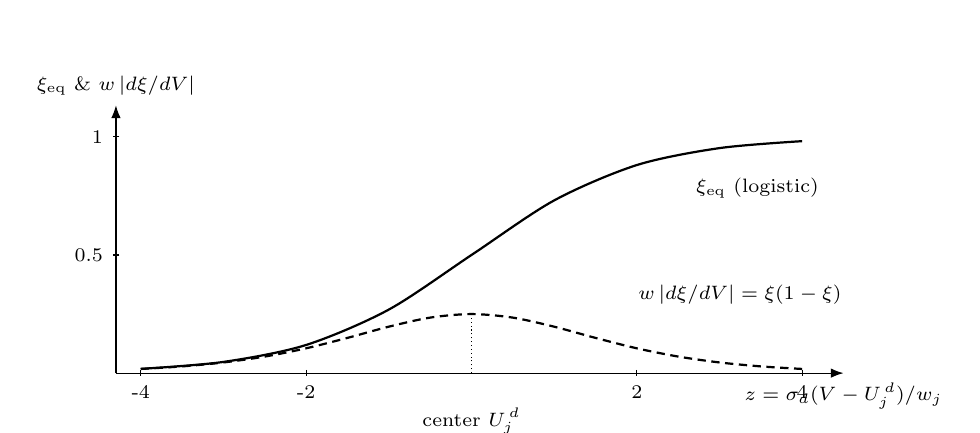
\begin{tikzpicture}[x=1.05cm,y=1.0cm]
% left axis: xi_eq (S-curve), right: dxi/dV bell — shared z-axis
\draw[-{Latex[length=1.6mm]}] (-4.3,0) -- (4.5,0) node[below,font=\scriptsize] {$z=\sigma_d(V-U_j^{\,d})/w_j$};
\draw[-{Latex[length=1.6mm]}] (-4.3,0) -- (-4.3,3.4) node[above,font=\scriptsize] {$\xi_\eq$ \&\ $w\,|d\xi/dV|$};
\foreach \xx in {-4,-2,2,4} {\draw (\xx,0.04) -- (\xx,-0.04) node[below,font=\scriptsize] {\xx};}
\draw (-4.26,3.0) -- (-4.34,3.0) node[left,font=\scriptsize] {1};
\draw (-4.26,1.5) -- (-4.34,1.5) node[left,font=\scriptsize] {0.5};
% xi_eq = 1/(1+e^-z) scaled by 3
\draw[thick] plot[smooth] coordinates {(-4,0.0540) (-3,0.1423) (-2,0.3576) (-1,0.8068) (0,1.5) (1,2.1932) (2,2.6424) (3,2.8577) (4,2.9460)};
\node[right,font=\scriptsize] at (2.6,2.35) {$\xi_\eq$ (logistic)};
% derivative xi(1-xi) max 0.25 scaled by 3 -> max 0.75
\draw[densely dashed,thick] plot[smooth] coordinates {(-4,0.0530) (-3.5,0.0854) (-3,0.1355) (-2.5,0.2103) (-2,0.3150) (-1.5,0.4474) (-1,0.5898) (-0.5,0.7050) (0,0.7500) (0.5,0.7050) (1,0.5898) (1.5,0.4474) (2,0.3150) (2.5,0.2103) (3,0.1355) (3.5,0.0854) (4,0.0530)};
\node[right,font=\scriptsize] at (1.9,1.00) {$w\,|d\xi/dV|=\xi(1-\xi)$};
\draw[densely dotted] (0,0)--(0,0.75);
\node[below,font=\scriptsize] at (0,-0.32) {center $U_j^{\,d}$};
\end{tikzpicture}
\caption{평형 진행률과 그 미분. 실선 $=\xi_\eq$ logistic(식~\eqref{eq:xieq}), 파선 $=$ 폭으로 규격화한
미분 $w_j|d\xi_\eq/dV|=\xi_\eq(1-\xi_\eq)$ — $z=0$(중심 $U_j^{\,d}$)에서 최대 $\tfrac14$ 인 종 모양. 이 종이
다음 절의 평형 peak 이고, 방향에 불변(양수)이다.}
\label{fig:logistic}
\end{figure}

% ====================================================================
\section{평형 peak — $|I|\to0$ 기준선 (N6)}\label{sec:eqpeak}
% ====================================================================
평형 진행률에서 곧바로 얻어지는 것이 평형 peak 모양 $\xi_\eq(1-\xi_\eq)/w$ 이다. 이것이 전류가 없을 때($|I|\to0$)의
기준선이며, 동역학 꼬리가 무시될 만큼 작을 때 곡선이 이 종으로 직접 환원되는 항이다.

\textbf{(a) 출발 — 전하 보존식.} 관측 $\dd Q/\dd V$ 는 전하 보존식 $Q_\cell q=Q_\bg(V_n)+\sum_jQ_j\xi_j$ 를 궤적
$q$ 로 미분해 닫힌다 — 양변을 $q$ 로 미분하면 $Q_\cell=C_\bg\,\dd V_n/\dd q+\sum_jQ_j\,\dd\xi_j/\dd q$ 이고,
$\dd V_n/\dd q$ 로 나누면 $\dd Q/\dd V_n=C_\bg+\sum_jQ_j\,\dd\xi_j/\dd V_n$ 이다. \textbf{(b) 연산 — logistic
미분의 종 항등식.} 평형 추종이면 $\dd\xi_j/\dd V_n$ 에 평형 기울기가 들어가고, $z\equiv\sigma_d(V-U_j^{\,d})/w_j$ 로
$\xi_\eq=(1+e^{-z})^{-1}$ 를 미분하면
\begin{equation}
\frac{\dd\xi_\eq}{\dd z}=\frac{e^{-z}}{(1+e^{-z})^2}
=\underbrace{\frac{1}{1+e^{-z}}}_{\xi_\eq}\cdot\underbrace{\frac{e^{-z}}{1+e^{-z}}}_{1-\xi_\eq}
=\xi_\eq(1-\xi_\eq)
\label{eq:belliden}
\end{equation}
— $\xi(1-\xi)$ 는 $\xi=\tfrac12$ 에서 최대 $\tfrac14$ 인 종이다. \textbf{(c) 중간식 — 연쇄율.} 연쇄율
$\dd z/\dd V=\sigma_d/w_j$ 를 곱하면 $\dd\xi_{\eq,j}/\dd V=\sigma_d\,\xi_\eq(1-\xi_\eq)/w_j$. \textbf{(d) 박스.}
이를 보존식 미분에 넣으면 전이 $j$ 의 평형 peak 이 닫힌다:
\begin{equation}
\frac{\dd\xi_{\eq,j}}{\dd V}=\frac{\sigma_d\,\xi_{\eq,j}(1-\xi_{\eq,j})}{w_j}
\;\Longrightarrow\;
\boxed{\;\Big(\frac{\dd Q}{\dd V}\Big)^\eq_j
=Q_j\,\frac{\xi_{\eq,j}(1-\xi_{\eq,j})}{w_j}
=Q_j\,\Big|\frac{\dd\xi_{\eq,j}}{\dd V}\Big|\;.}
\label{eq:eqpeak}
\end{equation}
이 값이 전이별로 합산되어 배경과 함께 $|I|\to0$ 극한을 이룬다 --- 단 $\gamma_j\ne0$ 이면 이 극한은 분기
중심 $U_j^{\,d}$ 에 남는 히스테리시스 잔존 극한이고, 분기 없는 가역 기준선($U_j$ 중심)과는
$\gamma_j\to0$ 에서만 일치한다(히스테리시스는 열역학적 — \S\ref{sec:hys}). 부호 — $\sigma_d$ 가 미분에서 한 번 들어오지만 peak 모양은
절댓값 $|\dd\xi/\dd V|=\xi_\eq(1-\xi_\eq)/w$ 로 양수이고 방향 불변이다($\xi(1-\xi)\ge0$). 세 양 — 위치 $=$ 중심
$U_j^{\,d}$, 순높이 $=Q_j/(4w_j)$($\xi=\tfrac12$ 에서 $\xi(1-\xi)=\tfrac14$), 배경 차감 면적 $=Q_j$
($\int_0^1\dd\xi=1$, 식~\eqref{eq:belliden} 의 종이 $\dd\xi_\eq$ 의 치환적분이라 면적 $1$) — 가 이 한 식에서 읽힌다.

이 식이 쓰이는 조건은 ``지연 길이가 격자에 비해 작을 때''다 — 다음 절(\S\ref{sec:lag}; 그 전에 아래 소절이
두-상 폭의 지위를 먼저 닫는다)이 그 지연 길이 $L_V$ 를 세우고, $L_V$ 가 격자
몇 칸보다 작으면(또는 동역학 입력이 없으면) 식~\eqref{eq:eqpeak} 의 평형 종으로 직접 환원된다. 이것이 $|I|\to0$ 환원이다.

\subsection{평형 델타가 실측 종이 되는 까닭 — broadening 과 폭 $w_j$ 의 지위}\label{sec:broadening}
평형 peak 식~\eqref{eq:eqpeak} 의 폭 $w_j=n_jRT/F$ 가 \emph{무엇을 예측하는지}는 전이마다 다르다. 이 절은
전이를 둘로 갈라 출발점을 점검하고, 두-상 전이에서 평형의 \emph{날카로운 선}이 실측의 \emph{유한 종}이 되는
까닭을 모델 안의 양들로 닫는다 — 결론은 \emph{두-상 폭 $w_j$ 는 평형 예측이 아니라 broadening 이 정하는
현상학적 자유 피팅 폭}이라는 것, 그리고 그 종에서 평형 전위$\cdot$입자 반경 분포를 역산하지 않는다는
것(아래 (c))이다.

\textbf{(a) 전이별 출발 — 애초에 종인 전이와 평형 델타인 전이.} 흑연 staging 전이는 평형 단일 입자 dQ/dV 의 모양부터
둘로 갈린다. 첫째 부류는 \emph{연속 고용체(solid-solution)} 전이다 — dilute$\to$stage4 영역과
4L$\to$3L$\cdot$3L$\to$2L 두 전이(각각 표~\ref{tab:staging} 의 $4\!\to\!3\cdot3\!\to\!2\mathrm L$ 행)다. 문헌의 L 접미 명명은 면내 질서가 풀린
액체상 stage 를 가리키며(그림~\ref{fig:staging} 의 stage 2L 과 같은 용법), 표의 정수 행 라벨과 같은 전이를
가리킨다. 이들은 plateau 가 없는 연속 등온선이라\cite{rsc2021}, 단일 입자 평형 dQ/dV 가 \S\ref{sec:width} 의 logistic 미분
종(식~\eqref{eq:belliden})으로 \emph{이미} 폭 $\sim n_jRT/F$ 의 종이다(정규용액 격자기체의 등온선 기울기
$\dd\xi/\dd V$, \S\ref{sec:dist}; Levi--Aurbach\cite{leviaurbach1999}) — 폭이 식~\eqref{eq:wbase} 의 평형
예측 그 자체라 ``왜 종이냐''는 물음이 생기지 않는다. 둘째 부류는 \emph{두-상 평탄역(plateau)} 전이다 —
$2\mathrm L\!\to\!2$($\mathrm{LiC_{12}}$)와 $2\!\to\!1$($\mathrm{LiC_6}$)은 $\Omega_j>2RT$ 의 상분리(\S\ref{sec:hys}
의 spinodal 문턱)라 평형 단일 입자가 \emph{델타에 가깝다}(Maxwell 공통접선이 plateau 를 한 전위로 모으면
$\dd q/\dd V\!\to\!\infty$). Maxwell 공통접선이 정의하는 것은 그 공통 전위의 \emph{값}까지이고, 실재 $N$-입자계가
그 값을 실현하는 \emph{경로}(순차 전환)는 아래 (iii-a) 의 Dreyer 통계역학이 답한다 — 둘은 같은 평탄역의 값과
경로로 양립한다. 곧 ``평형은 델타여야 하는데 실측은 종''이라는 물음은 \emph{이 두-상 두 전이에만} 해당하고,
나머지는 원래 종이다 — 폭의 지위를 따질 자리도 이 둘뿐이다.

\textbf{(b) 둘째 부류의 델타가 종이 되는 까닭 — broadening 의 세 출처.} 두-상 전이에서 폭을 만드는 것은 (Maxwell
공통접선이 그리는) plateau \emph{내부}의 단일 입자 평형이 아니라, \emph{측정 조건}과 plateau \emph{양끝}, 그리고
\emph{전극이 단일 입자가 아니라 입자 앙상블이라는 사실}이다. 성격이 다른 세 출처를 구분해 합성하며, 그 결과(평형 델타가
실측 종으로 펼쳐지는 그림)를 그림~\ref{fig:broadening} 에 둔다.

\emph{① 유한율속 비대칭 꼬리(동역학 몫).} 첫째는 이 문건이 이미 모델로 담은 출처로, \emph{전류가 켜야} 생긴다 — 유한
전류면 단일 입자라 하더라도 표면 진행률이 평형 목표를 뒤따르며 과전압 $\eta$ 가 진행 중에 변하고, peak 을 한쪽으로
밀며 꼬리를 늘인다. 이것이 바로 \S\ref{sec:lag}--\S\ref{sec:tail} 의 동역학 지연 길이 $L_{V,j}$ 와 인과 꼬리
$(\xi_\eq-\xi_\mathrm{lag})/L_{V,j}$ 이며, C-rate 가 오를수록 심해지고 $|I|\!\to\!0$ 에서
\emph{소멸}한다($L_V\propto|I|$ — \S\ref{sec:lag}; Fly 등\cite{fly2020}).

\emph{② 내재 $RT/F$ 폭(평형 잔여 몫).} 둘째는 plateau 양끝의 단상(solid-solution) 꼬리가 까는 내재 폭으로, plateau
양끝이 첫째 부류와 같은 연속 등온선이라 그 경계가 무한히 날카롭지 않고 폭 $\sim RT/F$ 규모(수십 mV order)로 번진 데서
온다(Levi--Aurbach\cite{leviaurbach1999}) — 이 몫은 전류와 무관한 \emph{평형 자체의 잔여 폭}이라 $|I|\!\to\!0$ 에서도
남는다. $RT/F\!\approx\!26$ mV 는 $n_j{=}1$ 의 척도일 뿐 하한이 아니다 — plateau 끝 유효 다중도 $n_j$ 가
$1$ 미만이면 잔여 폭은 그보다 작아질 수 있고, \S\ref{sec:width} 폭 폴백 중 두-상 두 전이의 출발값
0.014 V($2\mathrm L\!\to\!2$)$\cdot$0.012 V($2\!\to\!1$)와 모순되지 않는다. 단 \emph{현재 코드의 staging
출발값은 $n_j{=}1$ 고정}이라 실제 평가 폭은 $RT/F\!\approx\!25.7$ mV 이고 폭 값을 직접 지정하는 경로는 다중도
$n$ 입력을 배제해야 활성화된다 — $n_j\!<\!1$ 은 피팅이 내려갈 수 있는 여지이지 현재 출발 상태가 아니다.

\emph{③ 집합 다입자 통계역학(앙상블 몫) — 구조 무질서 근거는 흑연 두-상($\mathrm{LiC_{12}}\cdot\mathrm{LiC_6}$)에 한함.} 셋째는 앞 두 출처가
한 입자 안에서 일어나는 일이었던 것과 달리, \emph{전극이 $N$ 개 입자의 앙상블}이라는 데서 온다. 이 앙상블 몫은 성격이
다른 두 층으로 갈리므로, 평형 층(iii-a)을 먼저 세운 뒤 broadening 층(iii-b)을 그 위에 얹는다 — 둘을 섞으면 ``중심이
분포한다''는 잘못된 그림에 이르게 된다. 이 기작은 흑연 \emph{두-상}(turbostratic 무질서가 있는 흑연의 staging
plateau, $\mathrm{LiC_{12}}\cdot\mathrm{LiC_6}$)에 \emph{국한}하며, LCO 양극의 세 전이에는 흑연-특정 구조 무질서
근거를 옮기지 않고 일반 $\eta$ 분포(iii-b)로만 다룬다(LCO 의 평형 $U_j$ 입자 무관성은 흑연
GITT(galvanostatic intermittent titration technique)\cite{park2021} 의 직접 증거가 아니라 동형
\emph{가정}이다 — tier C 추정(신뢰 등급 범례는 \S\ref{sec:lco-map} 각주), LCO 단독 GITT 입자무관 OCP(open
circuit potential — 본 문건의 OCV 와 같은 반쪽전지 준평형 전위, 문헌 표기 따름) 확정 시 갱신).

\emph{(iii-a) 평형 — Dreyer 다입자 통계역학이 \emph{plateau 구조}를 만든다.} 단일 입자의 비단조(non-monotonic) 자유
에너지(정규용액 $\Omega>2RT$) 아래에서, $N$ 개 입자의 앙상블은 동시에 두-상으로 들어가지 않고 \emph{공통 전위}에서
\emph{순차로} 한 입자씩 전환한다(전위는 공통이고 전환 \emph{시점}만 순차다 — 입자별로 전위가 다른 것이 아니다) —
이미 전환을 마친 입자와 아직 시작 안 한 입자가 공존하며 셀 전위를 한 값에 묶어 두는
것이 거시적 \emph{평탄역}이다(삽입 전지 다입자 평형의 표준 그림; Dreyer 등\cite{dreyer2010}).
단일 입자 등온선이 비단조라 한 입자만 보면 불안정한 점프이지만, 앙상블이 순차 전환으로 그 점프를
평탄역으로 펴 \emph{평형 dQ/dV 가 한 전위의 델타에 모인다} — 이 층은 broadening 이 아니라 \emph{평탄역(델타) 자체의 기원}이다.

\emph{(iii-b) broadening — 그 평형 델타를 종으로 펴는 것은 \emph{apparent-U $=U_j+\eta$} 의 앙상블 분포다.} 관측되는 peak
전위는 평형 중심이 아니라 겉보기 전위 $U_\app=U_j+\eta$(평형 중심 $U_j$ 에 과전압$\cdot$국소 환경 항 $\eta$ 가 얹힌
값)이다. 핵심 정정 — \emph{평형 중심 $U_j$ 는 입자 무관 상수}로 \emph{가정}하고(흑연 하프셀 GITT 준평형 OCP 가 staging 전위를
입자 크기$\cdot$전극 형상과 무관한 상수로 주므로\cite{park2021} 마이크론 흑연에서 입자별 평형 $U_j$ 의 산포 $\approx0$ 으로 둔다 —
전극 수준 OCP 는 이를 시사할 뿐 단일입자 산포를 직접 분해하진 못한다), \emph{분포하는 것은 $\eta$}다 —
과전압$\cdot$국소 접촉 저항$\cdot$국소 환경(결정성$\cdot$흑연화도$\cdot$turbostratic 무질서가 \emph{유효 장벽$\cdot$국소
$\eta$} 를 입자별로 흩뜨림)에서 오는 \emph{비-크기$\cdot$비-사이즈} heterogeneity 다. 따라서 앙상블 통계 평균의 적분
변수는 평형 $U_j$ 가 아니라 \emph{apparent-U} $U_\app$ 이고, 그 밀도 $\rho(U_\app)$ 는 $\eta$ 분포가 정한다:
\begin{equation}
\Big\langle\frac{\dd Q}{\dd V}\Big\rangle_\mathrm{ens}
=\int \rho(U_\app)\;\Big(\frac{\dd Q}{\dd V}\Big)^\mathrm{single}_{U_\app}\,\dd U_\app,
\qquad U_\app=U_j+\eta,\ \ U_j=\text{const},
\label{eq:ensavg}
\end{equation}
곧 단일 입자 응답 $(\dd Q/\dd V)^\mathrm{single}_{U_\app}$(평형 델타에 ② 내재 폭이 얹힌 좁은 peak)을 \emph{겉보기 중심}
$U_\app$ 이 $\eta$ 만큼 분포한 앙상블 위로 \emph{forward} 합성한 것이다 — (iii-a) 평형 층 위에 얹힌
broadening 층이며, $\eta$ 의 \emph{입자간 산포}를 평균한다. 식~\eqref{eq:ensavg} 가 담는 것은
②(커널 내 내재 폭)$\otimes$③(앙상블 $\eta$ 산포)뿐이다 — ①(유한율속의 \emph{비대칭} skew)은 대칭 합성곱으로
표현되지 않으므로 별도 동역학 파라미터 $L_V$(N7$\cdot$N8, $|I|\!\to\!0$ 소멸)가 담당하고, 두-상 \emph{총}
broadening 은 $w_j(\text{②}\otimes\text{③})+L_V(\text{①})$ 로 묶인다(①의 전류 몫을 $w_j$ 가 다시 흡수하면
이중계산). $\eta$ 산포가 좁아져 $\rho\!\to\!\delta(U_\app-U_j)$ 면 식~\eqref{eq:ensavg} 는 평형 중심 $U_j$
의 단일 델타로 환원된다(③ 소멸).
엄밀히는 $\eta$ 중 순수 \emph{동역학} 몫은 ①처럼 $|I|\!\to\!0$ 에서 소멸하고, 결정성$\cdot$turbostratic 무질서 같은
\emph{구조성} 몫이 평형까지 남으면 그것은 조작적으로 작은 $U_j$ 산포와 구별되지 않는다 — 그 잔여 몫까지
$\approx0$($\eta$ 지배)에 묻는 것이 위 가정의 보수적 읽기이며, forward-only 처방에서 안전하다. \emph{단, 본 문건은 식~\eqref{eq:ensavg} 의 forward 통계 평균만
쓴다} — 측정된 종에서 $\rho(U_\app)$ 를 \emph{역산}하지 않는다(그 까닭은 아래 (c)).

세 출처의 몫은 한 식으로 정량화된다. ② 와 ③ 은 대칭 합성곱으로 겹치므로 분산(2차 모멘트)이 정확히
가법이다 — 합성곱의 분산 가법은 분포의 모양과 무관한 항등식이며, ① 의 단측 지수 꼬리도 총분산에는
$L_{V,j}^2$ 로 가법된다. 그럼에도 ① 을 별도 축으로 세우는 까닭은 그 몫이 왜도와 평균 이동을 동반하고
전류에 비례해 소멸하여($L_V\propto|I|$) 대칭 폭 $w_j$ 와 분리 식별되기 때문이다:
\begin{equation}
\underbrace{\sigma_\mathrm{sym}^{\,2}}_{\text{대칭 폭(분산)}}
\;=\;\underbrace{\frac{\pi^2}{3}\Big(\frac{n_jRT}{F}\Big)^{\!2}}_{\text{② 내재(logistic 분산)}}
\;+\;\underbrace{\sigma_\eta^{\,2}}_{\text{③ 앙상블 }\rho(U_\app)\text{ 산포}},
\qquad
\underbrace{\ell_\mathrm{tail}}_{\text{비대칭 꼬리 길이}}\;=\;L_{V,j}\;\propto\;|I|
\label{eq:widthbudget}
\end{equation}
(logistic 미분 종~\eqref{eq:belliden} 은 규격화하면 scale $w_j$ 의 logistic 분포 그 자체라 분산이
$\pi^2w_j^2/3$, 반높이 전폭(full width at half maximum, FWHM)은
$2\ln(3+2\sqrt2)\,w_j\approx3.53\,w_j$ 다 — $n_j{=}1$,
298 K 에서 $\approx91$ mV). 기호 규약을 명시하면 — 식~\eqref{eq:widthbudget} 의 $\sigma$ 는 모두
\emph{표준편차}(분산의 제곱근)이고, ② 항의 제곱근이 내재 몫의 표준편차
$\sigma_\mathrm{int}\equiv\pi n_jRT/(\sqrt3\,F)$ 이며, logistic scale(여기서는 $w_j$)과는
$\sigma=\pi w_j/\sqrt3$ 으로 환산된다. 성분비로 적으면
$\sigma_\mathrm{sym}/\sigma_\mathrm{int}=\sqrt{1+(\sigma_\eta/\sigma_\mathrm{int})^2}$ 이라 같은
비율이 scale 에도 그대로 적용된다. 실측 종에서 조작적으로 분리되는 것도 이 두 축이다: 대칭 폭은 피팅 폭 $w_j$ 가
②$\otimes$③ 을 한꺼번에 흡수하고(두 몫의 분리는 $\sigma_\eta$ 의 독립 측정 없이는 비유일 — (c)-(ii) 의
ill-posed 성질과 같은 뿌리), 비대칭 꼬리는 $L_{V,j}$ 가 담당하며 $|I|\!\to\!0$ 에서 소멸해 두 축이 전류
의존성으로도 갈린다. 그림~\ref{fig:widthbudget} 이 이 예산의 세 단계를 같은 축 위에 둔다 — 두-상 $w_j$ 가
②$\otimes$③ 을 흡수하는 현상학적 자유 피팅 폭이라는 \S\ref{sec:width} 이중지위의 \emph{두-상} 측을
떠받치는 물리가 바로 이것이다.

\begin{figure}[t]
\centering
\begin{tikzpicture}[x=0.72cm,y=22.0cm]
\draw[-{Latex[length=1.6mm]}] (-6.3,0) -- (10.8,0) node[below,font=\scriptsize] {$(V-U_j)/w_j$};
\draw[-{Latex[length=1.6mm]}] (-6.3,0) -- (-6.3,0.275) node[above,font=\scriptsize] {$\dd Q/\dd V$ (임의 단위)};
\foreach \xx in {-4,0,4,8} {\draw (\xx,0.004) -- (\xx,-0.004) node[below,font=\scriptsize] {\xx};}
% (0) equilibrium delta at plateau potential
\draw[-{Latex[length=1.8mm]},very thick] (0,0) -- (0,0.262);
\node[font=\scriptsize,align=center] at (-3.15,0.255) {평형 델타(Maxwell 전위)};
% (ii) intrinsic logistic-derivative bell, w=1
\draw[black!60] plot[smooth] coordinates {(-6,0.0025) (-5,0.0066) (-4,0.0177) (-3,0.0452) (-2,0.1050) (-1,0.1966) (-0.5,0.2350) (0,0.2500) (0.5,0.2350) (1,0.1966) (1.5,0.1491) (2,0.1050) (2.5,0.0701) (3,0.0452) (4,0.0177) (5,0.0066) (6,0.0025) (7,0.0009) (8,0.0003)};
\node[font=\scriptsize,black!60] at (2.55,0.205) {② 내재 $n_jRT/F$};
% (ii)x(iii) broadened bell, effective scale 1.6w
\draw[densely dashed] plot[smooth] coordinates {(-6,0.0140) (-5,0.0252) (-4,0.0438) (-3,0.0721) (-2,0.1082) (-1,0.1419) (-0.5,0.1525) (0,0.1562) (0.5,0.1525) (1,0.1419) (1.5,0.1264) (2,0.1082) (2.5,0.0895) (3,0.0721) (4,0.0438) (5,0.0252) (6,0.0140) (7,0.0077) (8,0.0042)};
\node[font=\scriptsize,align=left] at (-4.0,0.128) {②$\otimes$③ 분산 가법\\$\sigma_\eta=1.25\,\sigma_\mathrm{int}$, 유효 scale $1.6\,w_j$};
% (i) finite-rate skewed: C conv one-sided exp, L=1.5w
\draw[thick] plot[smooth] coordinates {(-6,0.0074) (-5,0.0134) (-4,0.0238) (-3,0.0408) (-2,0.0656) (-1,0.0959) (-0.5,0.1106) (0,0.1232) (0.5,0.1322) (1,0.1365) (1.5,0.1358) (2,0.1305) (2.5,0.1213) (3,0.1097) (4,0.0833) (5,0.0587) (6,0.0392) (7,0.0251) (8,0.0156) (9,0.0094) (10,0.0056)};
\draw[-{Latex[length=1.3mm]},gray] (4.4,0.093) -- (7.6,0.040);
\node[font=\scriptsize] at (6.8,0.098) {$+$① 지수 꼬리 $\ell=L_{V,j}$};
\end{tikzpicture}
\caption{두-상 broadening 의 폭 예산(식~\eqref{eq:widthbudget}; 좌표는 식 그대로의 수치 평가). 평형
델타(수직 화살)에 ② 내재 logistic 미분 종(폭 $w_j$, 가는 실선)이 얹히고, ③ 앙상블 $\eta$ 산포와의
합성곱이 분산 가법으로 종을 넓히며(예시 — $\eta$ 산포의 표준편차를 내재 몫의 $1.25$ 배로 두면
$\sigma_\mathrm{sym}=\sqrt{1+1.25^2}\,\sigma_\mathrm{int}\approx1.6\,\sigma_\mathrm{int}$, 같은
함수족이면 유효 scale $1.6w_j$ — 파선으로 표시), ① 유한율속이 한쪽 지수
꼬리(예시 $L_V=1.5w_j$ 와의 단측 합성곱 — 수치 적분)를 늘여 종을 소인 방향으로 민다(굵은 실선). 대칭
두 몫은 $w_j$ 하나에 흡수되고 비대칭 꼬리만 $L_{V,j}$ 로 분리된다.}
\label{fig:widthbudget}
\end{figure}

\textbf{(c) 이 절의 범위 — 유도로 닫는 경계.} (b) 는 broadening 의 \emph{설명}(forward 통계
평균)까지이며, 아래 세 가지는 본 절의 범위에 포함하지 않는다 — 각각 배제의 근거를 함께 둔다.
\begin{enumerate}[label=(\roman*),leftmargin=2.2em,itemsep=2.5pt]
\item \textbf{입자 \emph{사이즈}(반경) 효과 — 보편형을 먼저 두고, 실조건 수치로 배제한다.} 크기가 곡선에
들어오는 일반형부터 적는다. 반경 분포(particle size distribution, PSD) $p(r)$ 를 갖는 앙상블의 응답은
단일 입자 응답을 PSD 위로 합성한
\begin{equation}
\Big\langle\frac{\dd Q}{\dd V}\Big\rangle_\mathrm{PSD}
=\int p(r)\,\Big(\frac{\dd Q}{\dd V}\Big)^{\mathrm{single}}_{\,U_j+\Delta U(r),\ \tau(r)}\,\dd r
\label{eq:psdconv}
\end{equation}
이고, 반경은 두 채널로만 커널에 들어온다. 첫째는 열역학 채널 — 표면$\cdot$상경계 에너지가 평형 전위를
옮기는 Gibbs--Thomson 이동
\begin{equation}
\Delta U(r)\;=\;\frac{2\gamma V_m}{F\,r}
\label{eq:gibbsthomson}
\end{equation}
($\gamma$ = 계면 에너지[J/m$^2$] — 분기 축소 인자 $\gamma_j$(그림$\cdot$검산표에서는 $\gamma$ 로
약기)와 무관한 별개 기호, $V_m$ = 삽입상
몰부피)이고, 둘째는 동역학 채널 — 고체 확산 평형화 시간
$\tau(r)=r^2/D$ 의 분산이다. 이제 실조건 수치를 대입한다. \emph{열역학 채널}: 흑연 호스트 몰부피
$6M_\mathrm{C}/\rho_\mathrm{graphite}=6\times12.011/2.26\approx31.9$ cm$^3$/mol
($\rho_\mathrm{graphite}=2.26$ g/cm$^3$ 는 표준 물성값)에 삽입 팽창($\sim$10--13\%)을 얹으면
$V_m(\mathrm{LiC_6})\approx36$ cm$^3$/mol $=3.6\times10^{-5}$ m$^3$/mol 이고(상한 논증이라 큰 쪽을 쓴다),
계면 에너지는 $\gamma\sim0.1$--$1$ J/m$^2$ 스케일로 상정한다(수치의 전용 문헌 anchor 는 근거 미발견 —
tier C; 상분리 입자 전극의 계면 에너지 논의는 Cogswell--Bazant\cite{cogswell2012} 참조. 아래는 상한
$\gamma=1$ 을 쓰는 상한 논증이라 결과가 $\gamma$ 의 정확값에 둔감하다). 이를 취하면
전형 마이크론 흑연 $r=1$--$15\,\mu$m 에서
\[
\Delta U(1\,\mu\mathrm m)\;\le\;\frac{2\times1\times3.6\times10^{-5}}{96485\times10^{-6}}
\;\approx\;0.75\ \mathrm{mV},
\qquad
\delta U_\mathrm{PSD}\;=\;\frac{2\gamma V_m}{F}\Big(\frac{1}{r_{\min}}-\frac{1}{r_{\max}}\Big)
\;\approx\;0.20\ \mathrm{mV}
\]
($r_{\min}/r_{\max}=3/15\,\mu$m 예시). 폭에 기여하는 것은 이동의 절대값이 아니라 PSD 위 이동의
\emph{산포} $\delta U_\mathrm{PSD}$ 인데, 이는 실측 폭 $w\sim RT/F\approx25.7$ mV 의 $1\%$ 미만이고,
이동 절대값 기준으로도 상한 $\gamma$$\cdot$최소 $r$ 에서 $3\%$ 를 넘지 못한다. tier C 상정의 견고성을
명시하면 — $\Delta U\propto\gamma$ 라 상한을 다시 $5$ 배 과대 상정해도($\gamma=5$ J/m$^2$)
$\delta U_\mathrm{PSD}\approx1.0$ mV 로 결론(실측 폭 대비 수 \% 미만)은 불변이다. \emph{동역학 채널}:
흑연의 GITT 실측 확산계수 $D\approx10^{-11}$--$4\times10^{-10}$ cm$^2$/s\cite{park2021} 로 평형화
시간은 $\tau(5\,\mu\mathrm m)=r^2/D\approx6\times10^{2}$--$2.5\times10^{4}$ s 규모이나, 이
$\tau\propto r^2$ 분산은 $|I|\to0$ 평형 기준선에서 항등적으로 소멸하며(지연은 유한 전류의 산물,
\S\ref{sec:lag}), 유한 전류에서는 전이당 단일 유효 $L_V$(N7)의 입자별 산포로 들어오는 이차
보정 — 이미 부차적인 꼬리 폭의 산포 — 에 그친다. 따라서 마이크론 흑연에서 반경$\to$곡선 사상은 두 채널
모두 정량적으로 작고, 일반형~\eqref{eq:psdconv} 의 반경 의존이 커널에서 소거되어 PSD 적분은 항등이
되며, 앙상블에 남는 heterogeneity 는 비-크기 $\eta$ 산포 — 곧 식~\eqref{eq:ensavg} — 뿐이다.
(b)-③ 의 $\rho(U_\app)$ 를 \emph{비-크기} heterogeneity 전용으로
두는 것은 선언이 아니라 이 수치 유도의 따름 결과다. 크기 채널이 유의해지는 것은 $1/r$ 이 큰 나노
영역(상한 $\gamma$ 기준 $r\approx30$ nm 에서 $\Delta U\approx25$ mV; $\gamma\sim0.1$ 이면 그
십분의 일)뿐이며, 그 영역(과 양자가둠 밴드 shift 류)은 본 장의
범위에 포함하지 않는다. Dahn 등의 $x_{\max}=1-P$ 무질서
모델\cite{dahn1995}은 비-크기 구조 무질서가 실재함을 보이는 \emph{용량-한계 예시}일 뿐, inter-particle
$\eta$ 분포 형상을 정량하는 1차 근거는 아니다(분포 형상 tier C 근거미발견 — intra-particle site-blocking
식을 과대인용하지 않는다).
\item \textbf{dQ/dV$\to\rho(U_\app)$ 역산은 ill-posed 이므로 하지 않는다(forward-only).} (b)-③(iii-b) 의 ``peak $=$
단일 입자 커널 $\circledast$ 앙상블 분포 $\rho(U_\app)$''(식~\eqref{eq:ensavg})는 1종 Fredholm 적분방정식(distribution
of relaxation times 와 동형)이라, 정방향(분포$\to$peak)만 잘 정의되고 역방향은 정규화$\cdot$형태가정 없이는
비유일$\cdot$불안정하다 — 서로 다른 분포가 거의 같은 곡선을 준다. 따라서 $\eta$ heterogeneity 는
\emph{현상학적 폭 $w_j$ 에 흡수되는 것으로만} 두고 식~\eqref{eq:ensavg} 를 forward 로만 쓴다(분포는 폭을
\emph{넓힐} 뿐 평형 중심 $U_j$ 를 옮기지 않는다 — (b)-(iii-b) 의 GITT 한정과 동일\cite{park2021}).
\item \textbf{입자 \emph{크기 분포}(PSD) 위로 합성곱하는 다입자 \emph{기계장치}는 모델에 넣지 않는다.} 모델은
\emph{단일 유효 입자 $+$ 동역학 지연 $L_V$}(N7$\cdot$N8) 구조를 유지하고, 앙상블 무질서는
현상학적 $w_j$ 한 파라미터로 흡수된다 — 모델 차원은 늘지 않고, 늘어난 것은 (b)-③ 의 \emph{비-크기} 통계
평균 \emph{설명}뿐이다(크기$\to$폭 맵은 후속).
\end{enumerate}

\begin{keybox}
\textbf{broadening 한 줄.} 연속 전이(dilute$\cdot$4L$\to$3L$\to$2L)는 평형 단일 입자가 \emph{이미} 폭 $n_jRT/F$ 의 종이고,
두-상 전이($\mathrm{LiC_{12}}\cdot\mathrm{LiC_6}$)만 평형(plateau 내부) 델타가 유한 종이 된다 — 그 폭은 \emph{세}
출처가 정한다: ① \emph{전류가 켜는} 유한율속 비대칭 꼬리($L_V$, $|I|\!\to\!0$ 소멸) ② plateau 양끝의 \emph{평형 잔여}
내재 폭($\sim RT/F$, 전류 무관) ③ \emph{입자 앙상블}의 집합 통계역학 — 평형 층(Dreyer 순차 전환이 \emph{plateau 구조}를
만듦)과 broadening 층(그 평형 델타를 펴는 \emph{apparent-U $=U_j+\eta$} 의 입자간 $\eta$ 산포 $\rho(U_\app)$)으로 갈리며,
forward 평균 $\int\rho(U_\app)\,(\dd Q/\dd V)^\mathrm{single}\,\dd U_\app$(식~\eqref{eq:ensavg}; $\rho\!\to\!\delta$ 면
평형 중심 $U_j$ 의 단일 델타로 환원; 흑연-특정 구조 무질서 \emph{근거}는 흑연 두-상 한정 — LCO 는 일반
$\eta$ 산포로만, 본문 ③). 셋을 한꺼번에 흡수하는 것이 \emph{현상학적 자유 피팅 폭}이며 —
\emph{분포하는 것은 $\eta$(겉보기 중심 $U_\app$), 평형 중심 $U_j$ 는 입자 무관 상수로 움직이지 않는다}. 입자
사이즈(반경) 채널은 마이크론 흑연에서 정량적으로 무시 가능하여($\delta U_\mathrm{PSD}\ll w$,
식~\eqref{eq:gibbsthomson} 수치 유도 — 본문 (c)-(i)) 모델은 $\rho(U_\app)$ 역산$\cdot$PSD 크기 convolution
으로 확장하지 않는다(역문제 ill-posed$\cdot$forward-only).
\end{keybox}

\begin{figure}[t]
\centering
\begin{tikzpicture}[x=1.0cm,y=0.95cm]
% left: solid-solution transition (already a bell at equilibrium)
\begin{scope}
\draw[-{Latex[length=1.6mm]}] (-2.7,0) -- (2.7,0) node[below,font=\scriptsize] {$V$};
\draw[-{Latex[length=1.6mm]}] (-2.7,0) -- (-2.7,2.6) node[above,font=\scriptsize] {$dQ/dV$};
% equilibrium bell (already broad) — solid
\draw[thick] plot[smooth] coordinates {(-2.3,0.18) (-1.6,0.5) (-1.1,0.95) (-0.6,1.6) (-0.2,2.1) (0,2.2) (0.2,2.1) (0.6,1.6) (1.1,0.95) (1.6,0.5) (2.3,0.18)};
\node[font=\scriptsize,align=center] at (0,-0.7) {(a) solid-solution\\(dilute, 4L$\to$3L$\to$2L):\\equilibrium is already a bell};
\node[font=\scriptsize] at (1.35,1.7) {$w\!=\!nRT/F$};
\end{scope}
% right: two-phase transition (equilibrium delta -> measured bell via broadening)
\begin{scope}[xshift=6.4cm]
\draw[-{Latex[length=1.6mm]}] (-2.7,0) -- (2.7,0) node[below,font=\scriptsize] {$V$};
\draw[-{Latex[length=1.6mm]}] (-2.7,0) -- (-2.7,2.6) node[above,font=\scriptsize] {$dQ/dV$};
% equilibrium plateau-interior near-delta: tall NARROW (but finite edge width) — dashed
\draw[densely dashed,thick] plot[smooth] coordinates {(-0.32,0.0) (-0.18,0.7) (-0.08,1.9) (0,2.42) (0.08,1.9) (0.18,0.7) (0.32,0.0)};
\node[font=\scriptsize,align=center] at (-1.0,2.2) {eq.\ (plateau\\interior)};
% measured bell, skewed to higher V (finite-rate tail)
\draw[thick] plot[smooth] coordinates {(-2.3,0.12) (-1.6,0.34) (-1.1,0.66) (-0.6,1.1) (-0.2,1.5) (0.2,1.62) (0.5,1.5) (0.9,1.18) (1.3,0.82) (1.8,0.46) (2.3,0.24)};
\draw[-{Latex[length=1.3mm]},gray] (0.7,1.3)--(1.6,0.6);
\node[font=\scriptsize] at (1.45,1.15) {$\eta(t)$ tail (①)};
\node[font=\scriptsize,align=center] at (0,-0.7) {(b) two-phase ($\mathrm{LiC_{12}},\mathrm{LiC_6}$):\\near-delta $\to$ bell by broadening\\($w_j$ phenomenological)};
\end{scope}
\end{tikzpicture}
\caption{평형 모양과 broadening. (a) 연속 고용체 전이 — 평형 단일 입자 dQ/dV 가 이미 폭 $n_jRT/F$ 의
종(식~\eqref{eq:eqpeak}), broadening 불요. (b) 두-상 전이 — 평형은 plateau \emph{내부}에서 거의 날카로운
선(파선; 양끝 단상 꼬리 탓에 폭이 정확히 $0$ 은 아님)이고, 실측은 세 출처가 펼친 치우친 종(실선)이다:
① 유한율속 비대칭 꼬리(\S\ref{sec:lag}--\S\ref{sec:tail} 의 $L_V$, $|I|\!\to\!0$ 소멸),
② 전류 무관한 가장자리 내재 폭($\sim RT/F$),
③ 겉보기 중심 $U_\app=U_j+\eta$ 의 입자간 $\eta$ 산포를 forward 평균한 앙상블 몫(식~\eqref{eq:ensavg}).
①의 $\eta(t)$(한 입자의 시간 변화)와 ③의 입자간 $\eta$ 산포는 같은 과전압의 다른 평균이며, 평형 중심 $U_j$ 는
입자 무관 상수다 — 분포하는 것은 $\eta$. 세 출처의 지위와 한정(폭 $w_j$ 의 현상학적 지위$\cdot$흑연 두-상
국한$\cdot$$\rho(U_\app)$ 역산 금지$\cdot$사이즈 배제)은 본문 (b)$\cdot$(c).}
\label{fig:broadening}
\end{figure}

% ====================================================================
\section{동역학 지연 길이 $L_V$ (N7)}\label{sec:lag}
% ====================================================================
유한 전류에서는 평형 목표 $\xi_\eq$ 를 점유가 즉시 따라가지 못하고 뒤처진다 — 그 지연이 peak 의 꼬리다. 이 절은 그 지연을 전이당 하나의 길이 $L_{V,j}$ 로 닫는다 — 사슬
$\mathcal A\to\chi_d\to\Delta H_a^\eff\to L_q\to L_V$ 를, 운동방정식의 보편형에서 한 단계씩 닫는다.

\subsection{지연의 보편 방정식과 용량축 길이 $L_q$}
\textbf{(a) 출발 — 운동방정식을 용량축으로.} \S\ref{sec:width} 의 운동방정식 $\dd\xi_j/\dd t=k_j(\xi_{\eq,j}-\xi_j)$
을, 정전류에서 성립하는 $\dd q/\dd t=|I|/Q_\cell$ 로 나누면 $\dd\xi_j/\dd q=(Q_\cell k_j/|I|)(\xi_{\eq,j}-\xi_j)$.
\textbf{(b) 연산 — 지연 변수.} 지연 $r_j\equiv\xi_{\eq,j}-\xi_j$ 의 변화율 $\dd r_j/\dd q=\dd\xi_{\eq,j}/\dd q-\dd\xi_j/\dd q$
에 위 식을 넣으면 \textbf{(c) 중간식.}
\begin{equation}
\frac{\dd r_j}{\dd q}=\frac{\dd\xi_{\eq,j}}{\dd q}-\frac{Q_\cell k_j}{|I|}\,r_j,
\label{eq:Lqmid}
\end{equation}
\textbf{(d) 박스 — 용량축 길이 정의.} 계수의 역수가 용량축 지연 길이다:
\begin{equation}
\frac{\dd r_j}{\dd q}=\frac{\dd\xi_{\eq,j}}{\dd q}-\frac{r_j}{L_{q,j}},
\qquad \boxed{\;L_{q,j}=\frac{|I|}{Q_\cell\,k_j}\;.}
\label{eq:Lq}
\end{equation}
$L_{q,j}$ 는 요구($|I|/Q_\cell$)와 공급($k_j$)의 비 그 자체다 — 근본식의 세 인자가 전부 이 한 양을 통해 꼬리로
들어온다. 완화 속도 $k_j$ 는 평형 근방 선형 완화에서 정$\cdot$역 속도의 합이다 — detailed balance~\eqref{eq:db} 로
$r_j^-=r_j^+e^{-\mathcal A_j/RT}$ 이므로
\begin{equation}
k_j=r_j^++r_j^-=r_j^+\big(1+e^{-\mathcal A_j/RT}\big),
\qquad r_j^+\simeq k_0\,e^{-(\Delta G_{a,j}^\eff-\chi_d\mathcal A_j)/RT}\ (k_0=k_BT/h),
\label{eq:kuniv}
\end{equation}
이고, 괄호 인자 $(1+e^{-\mathcal A_j/RT})$ 가 역방향 몫의 전부다($\mathcal A\gtrsim3RT$ 면 $1$로 수렴한다). 이 두 인자가
아래 $L_q$ 평가식의 분모와 forward 지수를 각각 채운다.

\subsection{컷 affinity $\mathcal A$ — 꼬리 시작점의 구동력}
$L_q$ 는 전이당 한 점(꼬리 컷점 $q_a$)에서 \emph{상수로 동결}된다. \textbf{(a) 출발 — 컷의 정의.} 컷점은 원천
$\dd\xi_\eq/\dd q$ 가 정점의 일정 분율(약 $5\%$)로 떨어지는 좌표이고, \textbf{(b)(c) 연산$\cdot$중간식 — 컷의 구동력.}
컷은 점유 $\xi_\eq$ 자체가 아니라 그 \emph{미분} $\dd\xi_\eq/\dd q$ 의 $5\%$ 기준이며, logistic 미분 종의 $5\%$
폭이 중심에서 $\pm z_\mathrm{cut}\,RT/F$ 규모라 그곳의 구동력은 $\mathcal A=z_\mathrm{cut}\,n_jRT$($z_\mathrm{cut}=4.357$
— 이 $5\%$ 컷에 대응하는 선택값)다. \textbf{(d) 박스 — 상한과 함께.}
\begin{equation}
\mathcal A=\min\!\big(z_\mathrm{cut}\,n_j\,RT,\;A_\mathrm{cap}\,RT\big),
\qquad z_\mathrm{cut}=4.357,\ A_\mathrm{cap}=4.0\ (\text{기본}).
\label{eq:Acut}
\end{equation}
기본 상태($n_j{=}1$)에서는 $z_\mathrm{cut}n_jRT=4.357RT>A_\mathrm{cap}RT=4.0RT$ 라 상한이 걸려 실효
컷은 $z=4.0$(정점의 약 $7\%$)이고, $5\%$ 컷 분기는 $n_j<A_\mathrm{cap}/z_\mathrm{cut}\approx0.92$ 로
피팅될 때 활성화된다.
\emph{부호의 핵심} — 컷 affinity 의 \emph{크기}는
충$\cdot$방전 동일($n_j>0$ 라 항상 양수)이고, 방향은 아래 $\chi_d\cdot\Delta H_a^\eff$ 가 받는다. 방향 부호 $\sigma_d$ 를
$\min$ 안에 넣으면 충전에서 상한이 음수가 되어 물리적으로 무의미해지므로, 크기는 항상 양수로 두고 방향은 전달
계수 $\chi_d$ 로만 반영한다.

\subsection{방향별 전달 계수와 유효 장벽}
\textbf{(a) 출발 — 합-1 제약.} 전이상태가 정$\cdot$역 장벽을 비대칭으로 가르는 분율 $\chi\in[0,1]$ 의 합-1 제약
($\chi+\chi'=1$, 식~\eqref{eq:db} detailed balance 가 강제)에서, \textbf{(b)(c) 방향별 선택.} 방향별 전달 계수는
\begin{equation}
\chi_d=\chi_\mathrm{split}(\chi,\sigma_d)=
\begin{cases}\chi & \sigma_d\ge0\ (\text{방전})\\ 1-\chi & \sigma_d<0\ (\text{충전}).\end{cases}
\label{eq:chid}
\end{equation}
\textbf{(d) 유효 장벽.}
구동력에 평균장 $\mu$ 의 상호작용 몫(식~\eqref{eq:mu} 의 몫을 $\xi$ 좌표로 옮긴 $\Omega(1-2\xi)$ — $\theta=1-\xi$ 에서 부호 반전)을 마저 실으면
$\mathcal A_j=sF(V-U_j)-\Omega_j(1-2\xi_j)$ 다 — 이 상수 몫은 아래처럼 \emph{장벽}으로만 흡수되고, 컷점
판정(식~\eqref{eq:Acut})은 이상 몫 $sF(V-U_j)$ 로 남아 이중계산이 없다.
깊은 꼬리에서 방전은 $\xi\to1$ — 상호작용 몫
$-\Omega(1-2\xi)\to+\Omega$ — 이고, 충전은 $\xi\to0$ 거울이되 충전의 구동력은 리튬화 방향으로 부호가 뒤집힌
$-sF(V-U_j)+\Omega_j(1-2\xi_j)$ 라 같은 극한에서 상호작용 몫 $+\Omega(1-2\xi)\to+\Omega$ — 두 방향 모두
구동력의 상수 몫이 \emph{같은} $+\Omega$ 이고, 이것이 정방향 유효 장벽의 활성화 엔탈피로 흡수되어 유효값이 된다:
\begin{equation}
\boxed{\;\Delta H_{a,j}^\eff=\Delta H_{a,j}-\chi_d\,\Omega_j\;.}
\label{eq:dHeff}
\end{equation}
단, 이 보강이 꺼져 있으면(토글 옵션) 보강 없이 $\Delta H_a$ 를 그대로 쓴다.

\subsection{$L_q$ 의 평가와 전압축 환산 $L_V$}
\textbf{(a) 출발 — 정$\cdot$역 합과 Eyring prefactor.} 식~\eqref{eq:kuniv} 의 $k_j=r_j^+(1+e^{-\mathcal A_j/RT})$ 와
$r_j^+\simeq k_0e^{-(\Delta G_a^\eff-\chi_d\mathcal A)/RT}$($k_0=k_BT/h$)을 식~\eqref{eq:Lq} 의 $L_{q,j}=|I|/(Q_\cell k_j)$
에 넣으면 \textbf{(b)(c) 연산$\cdot$중간식 — $\Delta G_a^\eff=\Delta H_a^\eff-T\Delta S_a$ 로 갈라 적기.}
\begin{equation}
L_{q,j}=\frac{|I|}{Q_\cell}\cdot\frac{h}{k_BT}\cdot
\frac{e^{(\Delta H_{a,j}^\eff-T\Delta S_{a,j}-\chi_d\mathcal A)/RT}}{1+e^{-\mathcal A/RT}},
\label{eq:Lqmid2}
\end{equation}
\textbf{(d) 박스 — 특성 온도로 묶기.} 앞 인자를 $T_*\equiv|I|h/(Q_\cell k_B)$ 로 묶고 forward 지수를 분리하면
\begin{equation}
L_{q,j}=\frac{T_*}{T}\,\frac{\exp\!\big[(\Delta H_{a,j}^\eff-T\Delta S_{a,j})/RT\big]}{1+e^{-\mathcal A/RT}}
\,e^{-\chi_d\mathcal A/RT},
\qquad T_*\equiv\frac{|I|\,h}{Q_\cell\,k_B}.
\label{eq:Lqfull}
\end{equation}
\emph{암묵 전제 명시} — 식~\eqref{eq:Lqfull} 의
$\Delta H_a^\eff$ 는, 유효 장벽 보강이 켜져 있을 때만 식~\eqref{eq:dHeff} 의 $\Delta H_a-\chi_d\Omega$ 이고,
꺼져 있으면 그대로 $\Delta H_a$ 다. 전압축으로 옮기면, 컷점 OCV 기울기를 곱한다 — 꼬리 진폭이
용량축 $1/L_q$ 와 분모 $\dd V_n/\dd q$ 가 묶여 전압축 길이로 정리되는 것이다:
\begin{equation}
\boxed{\;L_{V,j}=\Big|\frac{\dd V}{\dd q}\Big|_{q_a}\,L_{q,j}\;.}
\label{eq:LV}
\end{equation}
\emph{부호의 핵심} — $\mathcal A$ 가 전이당 컷 상수로 동결되므로, \emph{실현되는} 미분은
$\partial\ln L_q/\partial V=0$ 이다(전이당 한 스칼라). 부등식 $\partial\ln L_q/\partial V<0$ 은 \emph{물리적 동기}로 읽어야
한다 — 만일 $\mathcal A$ 를 컷에 동결하지 않고 국소 구동력 $\mathcal A=\sigma_dF(V_n-U)$ 로 두면, 방전
기준($\sigma_d=+1$; 충전은 진행 방향 $V\!\downarrow$ 를 따라 같은 단조성) $V\!\uparrow\Rightarrow
\mathcal A\!\uparrow\Rightarrow$ 유효 장벽$\downarrow\Rightarrow L_q\downarrow$(꼬리 짧아짐)이고, 이 단조성이 ``꼬리 컷점을
원천 정점의 일정 분율로 잡는다''는 컷 규칙의 정당성이다. 한편 $|I|$ 의존은 동결 뒤에도 살아 있다 — $L_q\propto|I|$($T_*\propto|I|$)라 $|I|\to0$
에서 $L_V\to0$, 다음 절의 꼬리가 사라지고 평형 peak 으로 환원된다. 지연 길이를 직접 지정하면 동역학 계산을 우회해
그 값을 쓰고, $I\le0$ 이거나 활성화 엔탈피 입력이 없거나 컷점 OCV 기울기 $|\dd V/\dd q|_{q_a}$ 가
$0$(기본값$\cdot$미입력)이면 $L_V=0$ 이다.

N7 의 진행을 정리하면 — 다중도 $n_j$(입력 가드로 크기만 취함 — 정상 입력은 항상 양수)에서 컷 affinity $\mathcal A$(식~\eqref{eq:Acut})로,
방향별 전달 계수와 유효 장벽(식~\eqref{eq:chid}$\cdot$\eqref{eq:dHeff})으로, 용량축 지연 길이
$L_q$(식~\eqref{eq:Lqfull})로, 마지막으로 전압축 지연 길이 $L_V$(식~\eqref{eq:LV})로 이어지며, 전이당
\emph{상수} 하나(대표 $T_\rep\cdot$대표 $n$)로 한 번만 평가된다. 구현 대응은
부록~\ref{sec:appendix-code} 에 둔다.

% ====================================================================
\section{인과 기억 꼬리와 충전 격자 역전 (N8)}\label{sec:tail}
% ====================================================================
지연 길이 $L_{V,j}$ 가 충분히 크면($\ge$ 격자 몇 칸) 평형 종 대신 인과 기억 꼬리가 나타난다. 이 절이 그
합성곱과 충전에서의 격자 역전을 닫는다 — 부호 오류가 발생하기 쉬운 지점이므로 \S\ref{sec:signcheck} 에서 별도 검산한다.

\subsection{지수 기억 — 일반해의 이산형}
\textbf{(a) 출발 — 1계 선형 ODE.} 지연 방정식~\eqref{eq:Lq} 는 1계 선형이라 적분인자 $e^{q/L_{q,j}}$ 로 닫힌 해를 갖는다.
\textbf{(b) 연산 — 적분인자.} 양변에 $e^{q/L_{q,j}}$ 를 곱하면 좌변이 완전 미분으로 묶이고
\begin{equation}
\frac{\dd}{\dd q}\Big(r_j\,e^{q/L_{q,j}}\Big)
=e^{q/L_{q,j}}\Big(\frac{\dd r_j}{\dd q}+\frac{r_j}{L_{q,j}}\Big)
=e^{q/L_{q,j}}\,\frac{\dd\xi_{\eq,j}}{\dd q},
\label{eq:intfactor}
\end{equation}
\textbf{(c) 중간식 — 적분해 일반해.} $q_0$ 부터 적분하고 $e^{-q/L_{q,j}}$ 를 곱해 $r_j$ 를 꺼내면
\begin{equation}
r_j(q)=r_j(q_0)\,e^{-(q-q_0)/L_{q,j}}
+\int_{q_0}^{q}e^{-(q-q')/L_{q,j}}\,\frac{\dd\xi_{\eq,j}}{\dd q'}\,\dd q'
\label{eq:memory}
\end{equation}
— 초기 지연의 지수 감쇠 $+$ 과거 목표 변화율을 지수 커널 $K(\Delta q)=e^{-\Delta q/L_q}$ 로 가중한 \emph{기억}의
합성곱이다(계는 길이 $L_q$ 만큼의 최근 과거만 기억). \textbf{(d) 박스 — 이산 저역통과.} 이산 격자에서 이 1차 저역통과는
한 칸당 감쇠 $\rho=\exp(-\Delta_\mathrm{grid}/L_V)$ 의 점화식이다(연속해~\eqref{eq:memory} 를 격자 간격 $\Delta_\mathrm{grid}$
로 이산화하면 한 칸 전파가 $e^{-\Delta_\mathrm{grid}/L_V}$ 가중):
\begin{equation}
\xi_{\mathrm{lag},i}=\rho\,\xi_{\mathrm{lag},i-1}+(1-\rho)\,\xi_{\eq,i}
\label{eq:lowpass}
\end{equation}
이다. 초기값은 $\xi_{\mathrm{lag},0}=\xi_{\eq,0}$ —
패딩 격자 끝에서 $r(q_0)=0$, 곧 식~\eqref{eq:memory} 의 첫 항을 소거하는 선택이다. $L_V\le0$ 이거나 유한하지 않으면 저역통과는 항등이 되어 $\xi_\mathrm{lag}=\xi_\eq$ 다.
그림~\ref{fig:relaxode} 가 목표 $\xi_\eq$ 와 뒤처진 $\xi_\mathrm{lag}$, 그 차 $r=\xi_\eq-\xi_\mathrm{lag}$ 를 보인다.

\begin{figure}[t]
\centering
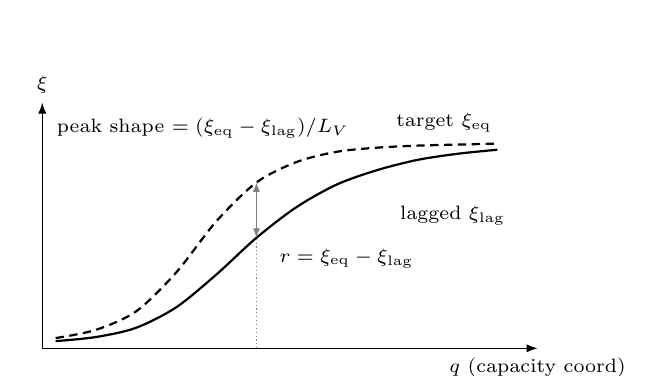
\begin{tikzpicture}[x=1.7cm,y=1.3cm]
% relaxation ODE: target xi_eq (step-like rise) and lagged response
\draw[-{Latex[length=1.4mm]}] (-0.1,0) -- (3.6,0) node[below,font=\scriptsize] {$q$ (capacity coord)};
\draw[-{Latex[length=1.4mm]}] (-0.1,0) -- (-0.1,2.4) node[above,font=\scriptsize] {$\xi$};
% target xi_eq: smooth rising sigmoid to 2
\draw[densely dashed,thick] plot[smooth] coordinates {(0,0.10) (0.3,0.18) (0.6,0.36) (0.9,0.74) (1.2,1.24) (1.5,1.62) (1.8,1.82) (2.1,1.92) (2.4,1.96) (2.7,1.98) (3.0,1.99) (3.3,2.0)};
\node[above,font=\scriptsize] at (2.9,2.02) {target $\xi_\eq$};
% lagged xi (follows behind, smaller, shifted right)
\draw[thick] plot[smooth] coordinates {(0,0.07) (0.3,0.11) (0.6,0.20) (0.9,0.40) (1.2,0.72) (1.5,1.08) (1.8,1.38) (2.1,1.60) (2.4,1.74) (2.7,1.84) (3.0,1.90) (3.3,1.94)};
\node[right,font=\scriptsize] at (2.5,1.30) {lagged $\xi_\mathrm{lag}$};
% gap arrow r = xi_eq - xi_lag at q=1.5
\draw[{Latex[length=1.2mm]}-{Latex[length=1.2mm]},gray] (1.5,1.08) -- (1.5,1.62);
\node[right,font=\scriptsize] at (1.60,0.88) {$r=\xi_\eq-\xi_\mathrm{lag}$};
\draw[densely dotted,gray] (1.5,0) -- (1.5,1.08);
\node[font=\scriptsize] at (1.1,2.15) {peak shape $=(\xi_\eq-\xi_\mathrm{lag})/L_V$};
\end{tikzpicture}
\caption{지연 ODE 의 완화. 파선 $=$ 평형 목표 $\xi_\eq(q)$, 실선 $=$ 점화식~\eqref{eq:lowpass} 으로 뒤처진
$\xi_\mathrm{lag}$. 둘의 차 $r=\xi_\eq-\xi_\mathrm{lag}$ 가 지연이고, peak 모양 $(\xi_\eq-\xi_\mathrm{lag})/L_V$
(바로 아래 \S 의 식~\eqref{eq:peakshape})는 이 차를 길이로 나눈 이산 미분이다. 이 매끈한 차분이 지연 진행률의
미분(평형 종$+$꼬리)으로 수렴하는 극한은 오히려 $L_V\gg\Delta_\mathrm{grid}$ 쪽이며 그림은 그 영역을 그린다 —
평형 종만으로의 환원($L_V\!\ll\!w$ 별도 필요)과 작은-$L_V$ 분기 스위치(식~\eqref{eq:branch})의 논증은 본문 \S\ref{sec:tail}.}
\label{fig:relaxode}
\end{figure}

\subsection{peak 모양 — 평형에서 지연을 뺀 것}
\textbf{(a)(b)(c) 출발$\cdot$연산$\cdot$중간식.} 진행률은 어디서나 $\xi_j=\xi_{\eq,j}-r_j$ 이고(지연 $r_j$ 는
일반해~\eqref{eq:memory} 가 전 구간 결정), 그 미분 $\dd\xi_j/\dd V=\dd\xi_{\eq,j}/\dd V-\dd r_j/\dd V$ 를 보존식
$\dd Q/\dd V=C_\bg+\sum Q_j\,\dd\xi_j/\dd V$ 에 넣은 ``평형 전환율에서 지연을 뺀 것''이다. 이산 격자에서 이 차분은
$(\xi_\eq-\xi_\mathrm{lag})$ 를 길이로 나눈 형태가 된다. \textbf{(d) 박스.}
\begin{equation}
\boxed{\;\text{peak shape}=\frac{\xi_{\eq}-\xi_{\mathrm{lag}}}{L_{V,j}}\;.}
\label{eq:peakshape}
\end{equation}
($\xi_\mathrm{lag}$ 는 점화식~\eqref{eq:lowpass}
의 출력). 이 차분이 매끈한 미분 $\dd\xi/\dd V$(지연 진행률의 미분 $=$ 평형 종$+$꼬리)로 수렴하는 극한은 $L_V\gg\Delta_\mathrm{grid}$ 쪽이다 —
이때 한 칸 감쇠 $\rho=e^{-\Delta_\mathrm{grid}/L_V}\to1$ 이라 점화식~\eqref{eq:lowpass} 의 커널이 길이 $L_V$ 의 진짜 1차
저역통과(미분 커널)로 살아나, $(\xi_\eq-\xi_\mathrm{lag})/L_V$ 가 평형 종에 꼬리를 더한 모양을 낸다(평형 종 $\dd\xi_\eq/\dd V$ 만으로 환원되려면 $L_V\!\ll\!w$ 가 더 필요하다 — $L_V\gg\Delta_\mathrm{grid}$ 는 수치 충실성 조건이지 평형 근접 조건이 아니다). \emph{반대로}
$L_V$ 가 작아지는 평형 회복은 이 차분의 극한이 \emph{아니다}: $L_V\to0$ 이면 $\rho\to0$ 이라 $\xi_\mathrm{lag}\to\xi_\eq$
(같은 칸 — 한 칸 지연이 아니다), 곧 분자 $(\xi_\eq-\xi_\mathrm{lag})\to0$ 과 분모 $L_V\to0$ 이 함께 사라지는 $0/0$ 이라
식~\eqref{eq:peakshape} 가 종으로 매끈히 환원되지 않는다. 그 작은 $L_V$ 의 평형 회복은 식~\eqref{eq:branch} 의 이산 분기가 담당한다 —
$L_V<\nu\,\Delta_\mathrm{grid}$ 면 식~\eqref{eq:peakshape} 를 평가하지 않고 평형 종 식~\eqref{eq:eqpeak} 을 직접 쓴다:
\begin{equation}
\text{peak shape}=
\begin{cases}
\xi_\eq(1-\xi_\eq)/w & L_{V,j}<\nu\,\Delta_\mathrm{grid}\ \text{(또는 비유한)}\quad[\text{평형, 식~\eqref{eq:eqpeak}}]\\[2pt]
(\xi_\eq-\xi_\mathrm{lag})/L_{V,j} & \text{그 외}\quad[\text{꼬리, 식~\eqref{eq:peakshape}}],
\end{cases}
\label{eq:branch}
\end{equation}
$\nu=2$ 다(지연이 격자 두 칸보다 짧으면 평형 종을 직접 쓴다). 이 전환은 \emph{매끈한 handoff 가 아니라
이산 모드 스위치}이다 — 문턱 $L_V=\nu\Delta_\mathrm{grid}$ 에서 꼬리 분기의 진폭과 평형 종의 진폭
($\propto 1/w$)이 정확히 같게 맞춰져 있지 않아 불연속이 생긴다 — 그 크기는 격자에 무관하게 $\nu$ 만의 닫힌 함수
$1-(1/\nu)\big/\!\big(e^{1/\nu}-1\big)$ (전이 면적은 정확히, 중심 peak 높이는 문턱 $L_V\!\ll\!w_j$ 인 기본 격자 영역에서 같은 인자)라, \emph{기본값 $\nu=2$ 에선 $\sim23\%$}(면적 $\approx0.77$)에 이르는 상당한 점프다.
이는 sub-grid 지연의 수치 불안정을 피하기 위한 실용적 선택이며($\nu$ 를 키우면
전환점이 더 깊은 꼬리로 밀려 점프가 $\approx50\%/\nu$ 급으로 줄어 — $\nu{=}8$: $6.1\%$, $\nu{=}10$: $4.9\%$, 곧 $5\%$ 이내로 낮추려면 $\nu\!\gtrsim\!10$ 이
필요하다\footnote{$L_V$ 를 최적화 도구로 피팅할 때 $L_V$ 가 이 문턱을 지나면 모델 곡선의 해당 전이
기여가 $\sim23\%$ 점프해 목적함수 landscape 에 불연속이 생긴다.}), 꼬리식 자신의 $L_V\to0$ 소멸
($0/0$)은 이미 평형 분기 영역에 들어가 꼬리식이 적용되지 않는 구간이다.

\subsection{★충전 격자 역전 — 인과 방향}
인과 합성곱~\eqref{eq:memory} 은 ``진행 방향의 과거''를 기억한다. 방전($\sigma_d=+1$)은 진행이 $V$ 증가 방향이라 격자
오름차순이 곧 시간 순서이고, 저역통과를 격자 그대로 적용한다. 충전($\sigma_d=-1$)은 진행이 $V$ 감소 방향 — 격자
오름차순의 \emph{역}이 시간 순서다. 따라서 충전은 격자를 뒤집어 필터하고 되돌린다:
\begin{equation}
\xi_\mathrm{lag}=
\begin{cases}
\mathrm{LowPass}(\xi_\eq) & \sigma_d\ge0\ (\text{방전})\\[2pt]
\mathrm{Reverse}\big[\mathrm{LowPass}(\mathrm{Reverse}[\xi_\eq])\big] & \sigma_d<0\ (\text{충전}).
\end{cases}
\label{eq:reversal}
\end{equation}
이 역전이 없으면 충전 꼬리가
\emph{미래}를 기억하는 비인과 신호가 되어 peak 가 엉뚱한 쪽으로 번진다. \emph{부호 결과} — 충전 $\dd Q/\dd V$ 는 방전의
거울상이고, peak 모양 $(\xi_\eq-\xi_\mathrm{lag})/L_V$ 는 양수를 유지한다(꼬리는 진행상 나중에 지나는
전위 쪽으로 — 방전은 높은 $V$, 충전은 낮은 $V$ 쪽으로 늘어진다). 그림~\ref{fig:reversal} 가 두 방향을 나란히 보인다.

\begin{figure}[t]
\centering
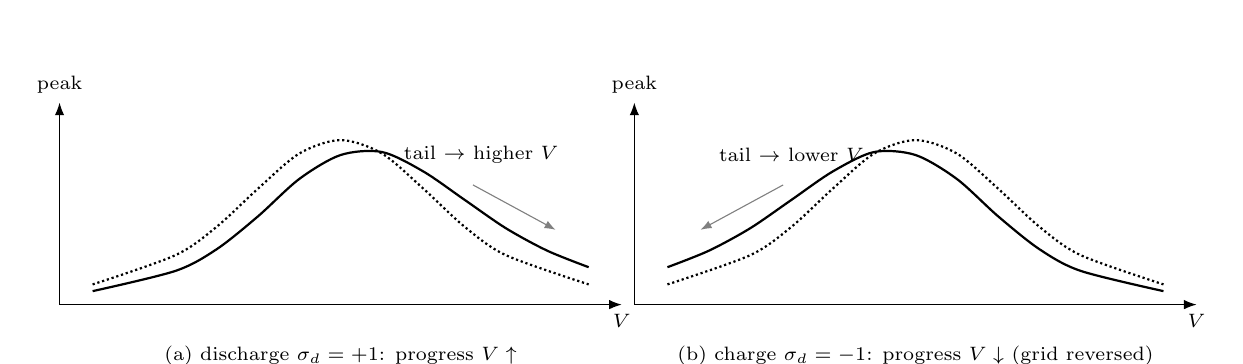
\begin{tikzpicture}[x=1.05cm,y=0.95cm]
% discharge panel (left)
\begin{scope}
\draw[-{Latex[length=1.6mm]}] (-3.4,0) -- (3.4,0) node[below,font=\scriptsize] {$V$};
\draw[-{Latex[length=1.6mm]}] (-3.4,0) -- (-3.4,2.7) node[above,font=\scriptsize] {peak};
% bell (equilibrium) dotted
\draw[densely dotted,thick] plot[smooth] coordinates {(-3,0.27) (-2,0.66) (-1.5,1.04) (-1,1.55) (-0.5,2.02) (0,2.2) (0.5,2.02) (1,1.55) (1.5,1.04) (2,0.66) (3,0.27)};
% discharge tail: shifted/broadened to higher V (right)
\draw[thick] plot[smooth] coordinates {(-3,0.18) (-2,0.45) (-1.5,0.74) (-1,1.18) (-0.5,1.68) (0,2.0) (0.5,2.04) (1,1.78) (1.5,1.4) (2,1.02) (2.5,0.72) (3,0.5)};
\draw[-{Latex[length=1.4mm]},gray] (1.6,1.6)--(2.6,1.0);
\node[font=\scriptsize] at (1.7,2.0) {tail $\to$ higher $V$};
\node[font=\scriptsize,below] at (0,-0.42) {(a) discharge $\sigma_d=+1$: progress $V\uparrow$};
\end{scope}
% charge panel (right)
\begin{scope}[xshift=7.3cm]
\draw[-{Latex[length=1.6mm]}] (-3.4,0) -- (3.4,0) node[below,font=\scriptsize] {$V$};
\draw[-{Latex[length=1.6mm]}] (-3.4,0) -- (-3.4,2.7) node[above,font=\scriptsize] {peak};
\draw[densely dotted,thick] plot[smooth] coordinates {(-3,0.27) (-2,0.66) (-1.5,1.04) (-1,1.55) (-0.5,2.02) (0,2.2) (0.5,2.02) (1,1.55) (1.5,1.04) (2,0.66) (3,0.27)};
% charge tail: mirror — broadened to lower V (left)
\draw[thick] plot[smooth] coordinates {(-3,0.5) (-2.5,0.72) (-2,1.02) (-1.5,1.4) (-1,1.78) (-0.5,2.04) (0,2.0) (0.5,1.68) (1,1.18) (1.5,0.74) (2,0.45) (3,0.18)};
\draw[-{Latex[length=1.4mm]},gray] (-1.6,1.6)--(-2.6,1.0);
\node[font=\scriptsize] at (-1.5,2.0) {tail $\to$ lower $V$};
\node[font=\scriptsize,below] at (0,-0.42) {(b) charge $\sigma_d=-1$: progress $V\downarrow$ (grid reversed)};
\end{scope}
\end{tikzpicture}
\caption{인과 꼬리의 방향. 점선 $=$ 평형 종($\xi_\eq(1-\xi_\eq)/w$, 방향 불변). 실선 $=$ peak shape
with tail. (a) 방전은 진행이 $V\!\uparrow$ 라 꼬리가 높은 $V$ 쪽으로 늘어진다(격자 그대로). (b) 충전은 진행이
$V\!\downarrow$ 라 격자를 뒤집어 필터한 뒤 되돌려(역순 저역통과의 재역순) 꼬리가 낮은 $V$ 쪽으로 — 방전의 거울. 두 경우 모두
peak 는 양수.}
\label{fig:reversal}
\end{figure}

% ====================================================================
\section{합산과 역보간 (N9)}\label{sec:sum}
% ====================================================================
전이별 peak 모양이 (식~\eqref{eq:branch} 의 두 분기로) 정해지면, 용량 가중을 곱해 작업 격자 위에 누적하고,
모든 전이가 끝나면 내부 전위 격자로 역보간한다. 보존식 $Q_\cell q=Q_\bg+\sum_jQ_j\xi_j$ 가
$\sum_jQ_j\xi_j$ 꼴이라 관측 ICA 는 배경과 전이별 기여의 선형 합이다 — 합산 자체는 보존식의 직접 미분이라 가정이
아니다(서로소 자리 분해가 전제):
\begin{equation}
\boxed{\;\frac{\dd Q}{\dd V}(V_n)\;=\;C_\bg\;+\;\sum_{j=1}^{N_p}Q_j\,
\big[\text{peak shape}_j\big]
\;=\;C_\bg+\sum_jQ_j\big[\text{평형 peak}-\text{지연 꼬리}\big]\;.}
\label{eq:sum}
\end{equation}
각 전이의 기여는 배경 위에 누적되고(배경은 합산 전에 먼저 깔림), 모든 전이가 끝나면 작업 격자에서
내부 전위 격자 $V_n$ 으로 역보간해 되돌린다. 스칼라 전위 입력은 한 점의 값으로 축약된다.

\subsection{staging 전이 초기값 — 피팅 출발점}
표~\ref{tab:staging} 가 네 전이 각 인자의 의미와 출발값이다(신뢰값이 아닌 \emph{초기값} — 사용자 피팅이
override 하는 것이 전제) — 이 표가 있어 ``이 문건만으로 곡선 재현 코드를 짤 수 있다''.

\begin{table}[t]
\centering
\renewcommand{\arraystretch}{1.25}
\caption{전이 초기값(흑연 staging 4건) — 출발점, 피팅으로 override. $U$ 는 $(\Delta H_\rxn,\Delta S_\rxn)$
정합 목표. 전위 anchor: $2\!\to\!1$($0.085$ V, Dahn\cite{dahn1991})$\cdot$$2\mathrm
L\!\to\!2$($0.120$ V, Ohzuku 등\cite{ohzuku1993})는 보고값과 정확 일치(2차 출처 경유 확인이라 tier B 로
보수 분류), $4\!\to\!3$($0.210$ V, Dahn\cite{dahn1991})은 근사 확인(tier B),
$3\!\to\!2\mathrm L$($0.140$ V)는 Ohzuku 보고 $\approx0.125$ V 와 $15$ mV 시료 의존
편차 안의 배치값(tier C — 문헌 간 $5$--$15$ mV 편차가 통상적). $\Delta S_\rxn$ 의 부호$\cdot$수십
J/(mol\,K) 스케일은 흑연 삽입 엔트로피 실측\cite{reynier2003} 과 정합(전이별 정밀값 아님 — tier B).}
\label{tab:staging}
\begin{tabular}{l c c c c c c c}
\toprule
stage & $U$ [V] & $\Delta H_\rxn$ & $\Delta S_\rxn$ & $Q$ & $\Omega$ & $\Delta H_a$ & $|\dd V/\dd q|_{q_a}$ \\
 &  & [J/mol] & [J/(mol\,K)] & [$Q_\cell$] & [J/mol] & [J/mol] & [V] \\
\midrule
$4\!\to\!3$   & 0.210 & $-11700$ & $+29.0$ & 0.10 & 6000  & 48000 & 0.30 \\
$3\!\to\!2\mathrm L$ & 0.140 & $-13500$ & $0.0$   & 0.12 & 8000  & 46000 & 0.30 \\
$2\mathrm L\!\to\!2$ & 0.120 & $-13100$ & $-5.0$  & 0.25 & 10000 & 44000 & 0.30 \\
$2\!\to\!1$   & 0.085 & $-13000$ & $-16.0$ & 0.50 & 13000 & 40000 & 0.30 \\
\bottomrule
\end{tabular}
\end{table}

각 전이는 폭 $w$ 폴백(0.020/0.016/0.014/0.012 V)과 $n=1$, $\Delta S_a=0$ 을 함께 갖는다. $\Delta H_\rxn/\Delta S_\rxn$
은 $U(298)$ 정합으로 정해졌고($U=(-\Delta H_\rxn+298.15\Delta S_\rxn)/F$ 가 표의 $U$ 와 $\pm1$ mV 안에서 정합 — $4\!\to\!3$ 행만 $0.2109$ 로 표시 자리수 경계), $\Delta H_a$ 는 저SOC(state of charge)$\to$
만충에서 감소하는 DFT(density functional theory) 활성화 경향\cite{persson2010,persson2010b} 에 맞춘
스케일이고(전이별 수치의 전용 문헌 anchor 는 근거 미발견 — 실측 계면 활성화 에너지의 문헌 범위
$25$--$59$ kJ/mol 와 겹치는 출발점), $|\dd V/\dd q|_{q_a}$ 는 컷 OCV 기울기(피팅), $\Omega$ 는 정규용액
추정(전이별 문헌 anchor 없음 — 피팅 출발점)이다.
초기 상태의 실현 크기를 정직하게 적어 두면 — 표의 $\Delta H_a$ 초기값에서 대표 조건(298 K$\cdot$C/10)의
$L_{V,j}$ 는 $10^{-10}$--$10^{-8}$ V 규모로 격자 문턱($\nu\Delta_\mathrm{grid}\sim10^{-4}$ V)에 크게 못
미치므로, $\gamma$ 미배정($=0$)$\cdot$$R_n=0$ 과 함께 \emph{초기 상태의 곡선은 꼬리$\cdot$분기 없는 평형
종 전용}이다(분기$\cdot$꼬리는 피팅 개방 후 활성). $k_0=k_BT/h$$\cdot$$\Delta S_a{=}0$ 전제에서 꼬리가
격자 문턱을 넘는 데는 $\Delta H_a\approx70$--$74$ kJ/mol(전이별$\cdot$기본 조건 기준), peak 폭에 견줄
가시적 꼬리에는 $\approx8\times10^4$ J/mol 급 또는 음의 $\Delta S_a$ 배정이 필요하므로, 인용 문헌
범위($25$--$59$ kJ/mol)는 절대값 anchor 가 아니라 경향 anchor 로 읽는다.
여기까지가 흑연(Part I)의 결과 사슬이다 — 다음 절부터 이 골격을 두 번째 전극 LCO 양극에 건다(Part II).

% ====================================================================
% ★ Part II 도입 절 신설(v1.0.14 P2.1 통합본).
%   원천: sec:lco-map(L301–355) 전문 이동(조정 4곳 선언) + sec:lco-hys ★분기 문단(L846–854)·
%         sec:lco-peak ★방향 문단+각주(L1426–1437) 흡수(원위치 대체 문안 = 본 맵 §5.3).
%   배치: Part II 블록 머리(P3.1 이동과 원자 결합 — §5.1).
% ====================================================================
\section{Part II --- LCO 양극: 전극-중립 골격에서 MSMR 통합까지}\label{sec:lco-intro}
Part I(흑연)이 세운 forward 골격은 처음부터 전극을 가리지 않도록 설계되었다. 이 절은 그 골격을 두 번째 전극
$\mathrm{LiCoO_2}$(LCO) 양극에 걸기 전에, Part II 전체가 전제할 세 가지 --- 무엇이 전극 무관인가
(\S\ref{sec:lco-map}), 방향 부호를 어떻게 먹이는가(\S\ref{sec:lco-direction}), 종반의 MSMR 동형은 어떤
모양으로 닫히는가(\S\ref{sec:lco-preview}) --- 를 한 곳에 고정한다. 이하 Part II 의 절들은 이 규약을
전제하고 각자의 자리에서 적용만 한다.

\subsection{전극-중립 골격 --- 무엇이 전극 무관인가}\label{sec:lco-map}
Part I 까지의 기호와 매핑은 \emph{전극을 가리지 않는다} --- 본론 사슬에서 host 물질이 들어가지 않는 식이
다섯이다:
\begin{enumerate}[label=(\arabic*),leftmargin=2.2em,itemsep=1pt]
\item 실험조건 매핑 식~\eqref{eq:n0map} --- 방향 부호 $\sigma_d$·전류 환산 $|I|=\text{c\_rate}\cdot Q_\cell$;
\item 삽입 평형 조건 식~\eqref{eq:eqcond} --- 반쪽반응
$\mathrm{Li}^++e^-+[\,]\rightleftharpoons\mathrm{Li}_{(\mathrm{host})}$ 의 전기화학 평형은 host 의 화학
정체를 상수 $\mu^0$ 와 입력값으로만 담는다(Part 0 \S\ref{sec:sm-electro} 의 유도에 host 항이 없다);
\item 정규용액 조성 자유에너지 식~\eqref{eq:gxi} --- ``동등한 자리에 리튬이 차고 빈다''는 가정 하나만 쓰며,
이는 LCO 의 팔면체 리튬 자리에도 문자 그대로 성립한다;
\item 평형 진행률 logistic 식~\eqref{eq:xieq} 와 폭 서식 $w_j=n_jRT/F$(식~\eqref{eq:wbase});
\item 전이 문법과 평형 peak --- 전이별 종 식~\eqref{eq:eqpeak} 와 그 전하 보존 합산(배경 $C_\bg$ 포함,
\S\ref{sec:eqpeak}$\cdot$\S\ref{sec:sum}).
\end{enumerate}
흑연 서술은 한 줄도 바뀌지 않으며(모든 흑연
식$\cdot$표$\cdot$부호는 불변), LCO 는 전이별 입력 파라미터를 교체하고 전자 엔트로피 항 하나를 추가한
두 번째 전극으로 들어온다. 본 문건이 다루는 범위는 \emph{코인 하프셀}(LCO vs Li metal) 단독이다 --- 전셀 합성
($\partial U_\cell=\partial U_\mathrm{cat}-\partial U_\mathrm{an}$)은 범위 밖이며(후속), 단전극(하프셀) 부호와 전셀
부호를 섞지 않는다.

\textbf{양극 부호 규약(흑연과 1:1 대칭).} LCO 하프셀 전위는 vs Li/Li$^+$ 로 $\sim$3.9--4.2 V 영역에 있다 — 흑연 음극의
$\sim$0.1 V 와 달리 \emph{높은} 전위다. 그러나 부호 골격은 같다: 셀 방전은 LCO 입장에서 \emph{리튬화}
(Li$^+$ 가 LCO 로 들어와 Co$^{4+}\!\to$Co$^{3+}$ 환원, $x$ 증가, 전위 하강)이고, 셀 충전은 \emph{탈리튬화}
($x$ 감소, 전위 상승)이다 — 단 이 문장은 \emph{화학 라벨}이고, 방향 의존 작용처(분극$\cdot$분기$\cdot$꼬리)에 들어가는
$\sigma_d$ \emph{슬롯 배정}은 \S\ref{sec:lco-direction} 의 탈리튬화 규약(LCO \emph{충전}$\mapsto\sigma_d{=}+1$)을
따른다. 평형 중심의 온도 의존은 관계식$\cdot$부호가 흑연과 동일하고 값만 전이별로 바뀐다(\S\ref{sec:lco-center}).
흑연에서 $\xi_j$ 가 탈리튬화 진행이었듯, LCO 양극에서 충전(탈리튬화)이 $\xi:0\!\to\!1$ 의 주 진행 방향이다 — 본 문건의
LCO 전이표는 그 충전 진행을 전위 오름차순으로 적는다.

흑연의 네 staging 전이 초기값(표~\ref{tab:staging})에 대응하는 LCO 초기값 리스트를 표~\ref{tab:lco-staging}
에 둔다(상세 \S\ref{sec:lco-preview}$\cdot$\S\ref{sec:lco-code}). 흑연이 4 staging 전이를 남기듯, LCO
하프셀(코인, $\le$4.2--4.5 V)은 세 전이를 남긴다\cite{xia2007}: $\sim$3.90 V 의 절연체$\to$금속 전이(insulator-to-metal transition, MIT), $\sim$4.05 V 와
$\sim$4.17 V 의 한 쌍 order--disorder 전이다(고전압 $\sim$4.55 V 의 O3$\to$H1-3 는 하프셀 상한이 $\le$4.2--4.5 V 면
범위 밖이라 옵션으로 둔다). 이 값들은 흑연과 마찬가지로 \emph{신뢰값이 아니라 초기값}이며\footnote{신뢰
등급 표기(본 문건 전역): tier A $=$ 1차 문헌의 정량 확정값, tier B $=$ 대표/부분 스케일 anchor 또는
2차 출처 경유 확인값(1차 원문 직접 확정 아님), tier C $=$ 추정$\cdot$placeholder(round-trip 피팅으로
갱신 예정).}(tier — 1차 문헌
Xia\cite{xia2007}$\cdot$Reynier\cite{reynier2004}$\cdot$Motohashi\cite{motohashi2009} 에서 읽은 출발점), 우리 시료 데이터로
피팅해 override 하는 전제다.

\begin{table}[t]
\centering\footnotesize
\renewcommand{\arraystretch}{1.3}
\caption{LCO 하프셀 전이 초기값(3건, vs Li metal) — 출발점, 피팅으로 override. $x$ 는
$\mathrm{Li}_x\mathrm{CoO_2}$ 의 리튬 함량. ``성격''은 상전이 유형, ``전자항''은 \S\ref{sec:lco-electronic} 의 MIT
게이트 발현 여부. 흑연 표~\ref{tab:staging} 와 같은 자리(전위$\cdot$성격$\cdot\Delta S$), 양극 부호.
★시연값($U{=}3.930/3.880/4.050$ V; 전자항은 T1$=$MIT dict 에
$x_\mathrm{MIT}{=}0.85$ 물리 anchor 로 배정)은
\emph{tier-C 시연 초기값}으로, $U$·$\Delta S_\rxn$ 시연값은 본 표의 물리 anchor(T1 MIT $\sim$3.90 V$\cdot$T3 $\sim$4.17 V·config 값)와
별개라 round-trip 피팅으로 정합한다. 또한 현 구현은 $\Delta S_e$ 를 기준온도 $T_\mathrm{ref}$ 에서
동결한 상수 오프셋으로 넣어(단일-기준 근사) peak 를 목표 전위에 둔다(조성 매핑$\cdot$다온도 $T^2$ 곡률
과제는 \S\ref{sec:lco-code}).}
\label{tab:lco-staging}
\begin{tabular}{@{}p{0.155\textwidth} c p{0.085\textwidth} p{0.165\textwidth} p{0.255\textwidth} p{0.115\textwidth}@{}}
\toprule
전이 & $U_j$ [V] & $x$ 범위 & 성격 & $\Delta S_{\rxn,j}^\mathrm{cat}$ 초기값 & 전자항 \\
\midrule
T1 (MIT)              & $\sim$3.90        & 0.94--0.75 & insulator$\to$metal       & config $+\,\Delta S_e$ 게이트 ON & \textbf{발현(핵심)} \\
T2 (order--disorder a)& $\sim$4.05        & $\approx$0.55 & hex$\to$monoclinic 정렬 & config 주도($\approx$0.47 J/(mol\,K); 배정 tier C) & 미발현 \\
T3 (order--disorder b)& $\sim$4.17--4.20  & $\approx$0.48 & monoclinic$\to$hex      & config($\approx$1.49 J/(mol\,K); 배정 tier C) & 미발현 \\
\midrule
(T4)                  & $\sim$4.55        & $\approx$0.2 & O3$\to$H1-3              & --- & (고전압, 범위 밖) \\
\bottomrule
\end{tabular}
\end{table}

흑연이 네 전이마다 $(\Delta H_\rxn,\Delta S_\rxn,Q,\Omega,\Delta H_a,\dots)$ 파라미터 묶음을 갖듯,
LCO 전이도 같은 파라미터 구조를 갖되 값만 표~\ref{tab:lco-staging} 의 양극 영역으로 바뀐다. 단 하나의 구조적 차이는 T1 에
흑연엔 없는 \emph{전자 엔트로피 항} $\Delta S_e(x,T)$ 가 더해지는 것이며(MIT 고유), 이것이 \S\ref{sec:lco-electronic}
의 새 절이다. N1--N5 구간에서 흑연과 LCO 는 \emph{같은 식}을 공유하므로 --- Part I 은 흑연으로 식을 세웠고,
Part II 의 절들은 LCO 파라미터를 끼워 넣는 순서로 간다.

\subsection{방향 규약 --- $\sigma_d$ 입력 슬롯의 물리 내용은 탈리튬화 여부다}\label{sec:lco-direction}
평형 중심$\cdot$폭$\cdot$평형 종은 방향과 무관하고, $\sigma_d$ 가 모델에 들어가는 작용처는 셋뿐이다 ---
분극(\S\ref{sec:pol})$\cdot$분기(\S\ref{sec:hys})$\cdot$꼬리(\S\ref{sec:tail}). 세 작용처 모두에서 이 슬롯이
실어 나르는 물리 내용은 셀 방향 라벨이 아니라 다음 한 줄이다:
\begin{equation}
\boxed{\;\begin{aligned}
&\sigma_d=+1\ \Leftrightarrow\ \text{탈리튬화(산화, $\xi:0\!\to\!1$, 전위 상승 진행)}:\\
&\quad\text{흑연 하프셀 --- 방전}\mapsto+1,\qquad \text{LCO 하프셀 --- 충전}\mapsto+1\;.
\end{aligned}}
\label{eq:lco-sigmaslot}
\end{equation}
흑연도 LCO 도 탈리튬화에서 하프셀 전위가 \emph{오른다}(흑연 $\sim$0.08$\to$0.21 V, LCO
$\sim$3.9$\to$4.2 V)는 사실이 이 규약을 전극-중립으로 만들고, 그림~\ref{fig:lco-dirmap} 이 이 대응이다.
이렇게 읽으면 세 작용처의 부호가 흑연과 1:1 로 유지된다:
\begin{enumerate}[label=(\alph*),leftmargin=2.2em,itemsep=1pt]
\item \emph{분극}(식~\eqref{eq:vn}) --- $\sigma_d=+1$(산화 전류)에서 $V_\app>V_n$: 흑연 방전과 LCO 충전이
같은 부호로 성립;
\item \emph{분기}(식~\eqref{eq:Ubranch}; LCO 대입형은 \S\ref{sec:lco-hys}) --- 탈리튬화 가지가 위
($+\tfrac12$), 리튬화 가지가 아래($-\tfrac12$): 과주행 기하(그림~\ref{fig:hysloop} --- 탈리튬화는 상승
가지 극대 $\xi_s^-$ 까지, 리튬화는 극소 $\xi_s^+$ 까지)가 전극 무관한 이중웰 성질이라, ``탈리튬화 peak 가
높은 전위 쪽''(흑연 $U^{\dis}>U^{\chg}$ 와 동일한 물리)이 LCO 에서도 유지된다;
\item \emph{꼬리}(식~\eqref{eq:reversal}) --- 꼬리는 진행의 시간상 뒤쪽으로 늘어지므로, $\sigma_d=+1$
(진행 $=$ 전위 오름)은 격자 오름차순이 곧 시간 순서라 역전이 불요하고 $\sigma_d=-1$ 은 격자를 뒤집어
필터한다: LCO 충전이 흑연 방전과, LCO 방전이 흑연 충전과 같은 처리를 받는다.
\end{enumerate}
LCO 의 $\Omega_j^\mathrm{cat}$·동역학 키가 배정되기 전에는 세 작용처 중 실질 활성이 분극뿐이며, 이는
\S\ref{sec:lco-hys} 의 two-phase calibration 지위 그대로다.

\textbf{층위 구분(모순 아님).} \S\ref{sec:lco-map} 의 ``셀 방전 $=$ LCO 리튬화'' 서술은 셀 방향
\emph{라벨}의 의미론(어느 셀 동작이 어느 화학 방향인가)이고, 본 절의 규약~\eqref{eq:lco-sigmaslot} 은 모델
\emph{입력 슬롯}에 그 라벨이 아니라 탈리튬화 여부를 대입한다는 적용 규칙이다 --- 두 서술은 층위가 달라 모순이
아니다.

\textbf{평형 종의 불변(방향이 가르는 것과 가르지 않는 것).} 평형 종 자체는 이 선택에 불변이다 --- 같은
중심$\cdot$폭에서 $1-\xi_\eq^{(\sigma_d)}=\xi_\eq^{(-\sigma_d)}$(여집합 교환; 식~\eqref{eq:xieq} 의 지수
부호 반전 그 자체이며, \S\ref{sec:lco-code} 의 변환 사전이 식으로 닫는다)이고 종 $\xi(1-\xi)$ 는 이 교환에
불변이라, 평형 peak 는 어느 읽기로도 같다. 방향 읽기가 갈라놓는 것은 오직 세 작용처 ---
분극$\cdot$분기$\cdot$꼬리 --- 다. 이 구분이 Part II 전체의 부호 실수를 막는 가드다.

\begin{figure}[t]
\centering
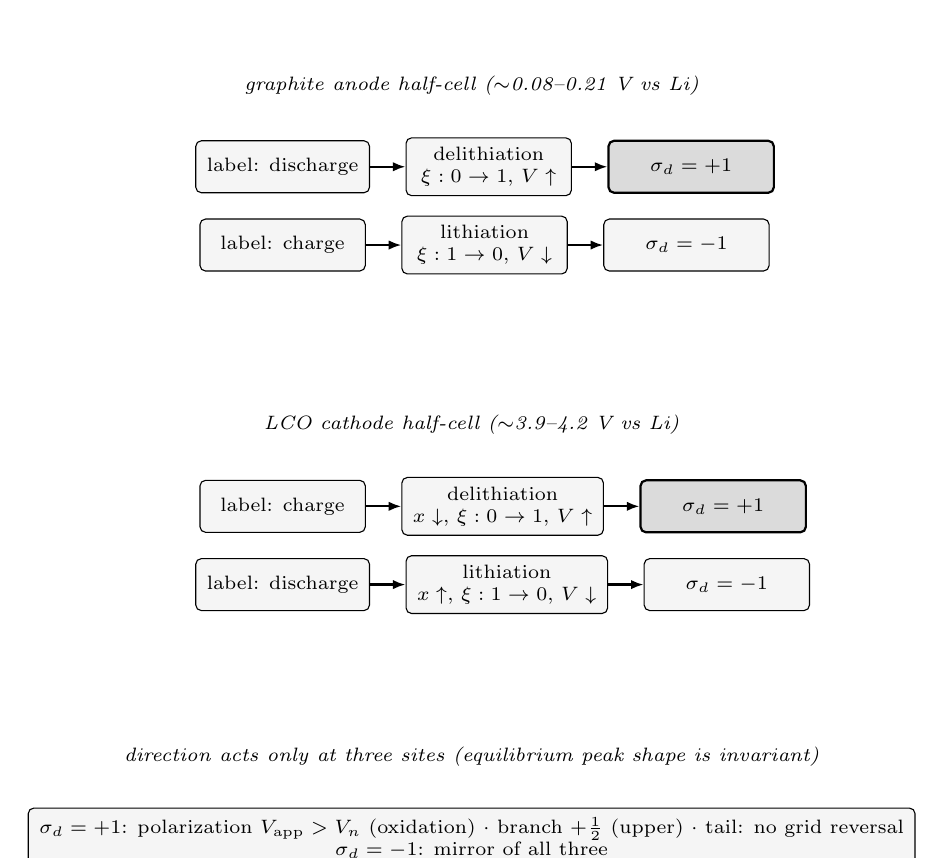
\begin{tikzpicture}[
  node distance=3.2mm and 4.5mm,
  lab/.style={draw,rounded corners=2pt,minimum height=6.6mm,minimum width=21mm,inner xsep=4pt,font=\scriptsize,align=center,fill=black!4},
  slotP/.style={lab,fill=black!14,thick},
  slotM/.style={lab,fill=black!4},
  hdr/.style={font=\scriptsize\itshape,align=center},
  ar/.style={-{Latex[length=1.6mm]},thick}]
% ---- graphite anode half-cell ----
\node[hdr] (gh) {graphite anode half-cell ($\sim$0.08--0.21 V vs Li)};
\node[lab,below=4.5mm of gh,xshift=-24mm] (gd) {label: discharge};
\node[lab,below=of gd] (gc) {label: charge};
\node[lab,right=of gd] (gdd) {delithiation\\$\xi:0\to1$, $V\uparrow$};
\node[lab,right=of gc] (gcc) {lithiation\\$\xi:1\to0$, $V\downarrow$};
\node[slotP,right=of gdd] (gp) {$\sigma_d=+1$};
\node[slotM,right=of gcc] (gm) {$\sigma_d=-1$};
\draw[ar] (gd)--(gdd); \draw[ar] (gdd)--(gp);
\draw[ar] (gc)--(gcc); \draw[ar] (gcc)--(gm);
% ---- LCO cathode half-cell ----
\node[hdr,below=17mm of gc,xshift=24mm] (lh) {LCO cathode half-cell ($\sim$3.9--4.2 V vs Li)};
\node[lab,below=4.5mm of lh,xshift=-24mm] (lc) {label: charge};
\node[lab,below=of lc] (ld) {label: discharge};
\node[lab,right=of lc] (lcc) {delithiation\\$x\downarrow$, $\xi:0\to1$, $V\uparrow$};
\node[lab,right=of ld] (ldd) {lithiation\\$x\uparrow$, $\xi:1\to0$, $V\downarrow$};
\node[slotP,right=of lcc] (lp) {$\sigma_d=+1$};
\node[slotM,right=of ldd] (lm) {$\sigma_d=-1$};
\draw[ar] (lc)--(lcc); \draw[ar] (lcc)--(lp);
\draw[ar] (ld)--(ldd); \draw[ar] (ldd)--(lm);
% ---- action sites ----
\node[hdr,below=16mm of ld,xshift=24mm] (ah) {direction acts only at three sites (equilibrium peak shape is invariant)};
\node[lab,below=4mm of ah,minimum width=96mm,align=center] (act)
 {$\sigma_d=+1$: polarization $V_\app>V_n$ (oxidation) $\cdot$ branch $+\tfrac12$ (upper) $\cdot$ tail: no grid reversal\\
  $\sigma_d=-1$: mirror of all three};
\end{tikzpicture}
\caption{충$\cdot$방전 라벨과 탈리튬화 방향의 대응. $\sigma_d$ 슬롯의 물리 내용은 셀 라벨이
아니라 ``작동 전극의 탈리튬화 $=+1$''(식~\eqref{eq:lco-sigmaslot})이다 --- 흑연 하프셀은 방전이, LCO
하프셀은 충전이 $\sigma_d=+1$ 슬롯(음영 상자)에 간다. 방향은 분극$\cdot$분기$\cdot$꼬리 세 작용처에만
작용하고 평형 종은 $\xi\leftrightarrow1-\xi$ 교환에 불변이다.}
\label{fig:lco-dirmap}
\end{figure}

\subsection{MSMR 대응 개관 --- 같은 logistic, 같은 부호 규약}\label{sec:lco-preview}
MSMR 모델은 양극 조성을 전위의 전이별 logistic 합으로 적는 표준
파라미터화라, Part II 종반에서 Ch1 곡선 클래스와 1:1 사전 --- $U\leftrightarrow V$,
$U_j^0\leftrightarrow U_j^{\,d}$, $\omega_j\leftrightarrow w_j$, $X_j\leftrightarrow Q_j$, $f=+\sigma_d$ ---
으로 맞물린다($f$ 는 원계열의 $F/RT>0$ 를 폭에 흡수하고 지수에 남는 방향 부호 인자). 이 가운데
$f=+\sigma_d$ 는 같은 물리량끼리 짝짓는 대응(pairing) 하의 유일해이며, 그 유도와 가드(``함수형 동형 $\ne$ 물리량
동일'')$\cdot$박스는 \S\ref{sec:lco-code} 가 닫는다.

\subsection{LCO 평형 중심과 $\partial U_j/\partial T$ — 양극 부호}\label{sec:lco-center}
\textbf{(a) 출발 — 전극-중립 골격의 세 진입.}
\S\ref{sec:center} 의 평형 중심 유도에는 어느 다리에도 ``흑연''이라는 물질 고유 항이 없다 —
(i) 실험조건 매핑 식~\eqref{eq:n0map} 의 방향 부호$\cdot$전류 환산
$\sigma_d=\pm1$, $|I|=\text{c-rate}\times Q_\cell$ 은 삽입형 전극이면 종류를 가리지 않고, (ii) 전기화학 평형
조건 식~\eqref{eq:eqcond}($\mu_\mathrm{Li}(\theta_\eq)=\mu^0-sF(V-U),\ \Delta G_j=-sFU_j$)는 삽입
반쪽반응 $\mathrm{Li}^++e^-+[\,]\rightleftharpoons\mathrm{Li}_{(\text{host})}$ 의 전기화학 평형
(식~\eqref{eq:eqbalance})에서 나와 host 의 화학 정체가 상수 $\mu^0$ 와 반응 몫 입력값으로 흡수되며,
(iii) 비배치 몫 $\Delta G_j=\Delta H_{\rxn,j}-T\Delta S_{\rxn,j}$ 은 반응 종에 무관한 열역학 항등식이라,
LCO 로 넘어갈 때 이 세 자리에 들어가는 것은 전이 집합과 입력값의 치환뿐이다:
\begin{equation}
j\in\mathcal J_\mathrm{LCO}=\{\mathrm{T1},\mathrm{T2},\mathrm{T3}\},\qquad
(\Delta H_{\rxn,j},\Delta S_{\rxn,j})\ \longmapsto\
(\Delta H_{\rxn,j}^\mathrm{cat},\Delta S_{\rxn,j}^\mathrm{cat}).
\label{eq:lco-n0sub}
\end{equation}
곧 $\sigma_d$ 는 방향 선택 슬롯에 남고, 평형 중심 $U_j(T)$ 의 Gibbs 환산식에는 새 양극 부호가 끼지 않는다.

\textbf{(b) 연산 — 평형 조건에 반응 자유에너지 대입.}
전이 $j$ 의 비배치 반응 자유에너지 $\Delta G_j^\mathrm{cat}=\Delta H_{\rxn,j}^\mathrm{cat}
-T\Delta S_{\rxn,j}^\mathrm{cat}$ 를 식~\eqref{eq:eqcond} 의 $\Delta G_j=-sFU_j$($s=+1$)에 넣으면
\[
\Delta H_{\rxn,j}^\mathrm{cat}-T\Delta S_{\rxn,j}^\mathrm{cat}=-F\,U_j^\mathrm{cat}(T),
\]
곧 흑연 식~\eqref{eq:Ujmid} 과 글자 그대로 같은 식에 상첨자 $\mathrm{cat}$ 만 붙는다.

\textbf{(c) 중간식 — 중심과 온도 미분(이중 경로 교차검증).}
(b)를 $U_j^\mathrm{cat}$ 로 이항하면 $U_j^\mathrm{cat}(T)=(-\Delta H_{\rxn,j}^\mathrm{cat}
+T\Delta S_{\rxn,j}^\mathrm{cat})/F$ 로 흑연 식~\eqref{eq:Uj} 와 같은 함수형이고, 온도 계수는 두 독립
경로가 같은 값에 닿는다. \emph{경로 1(직접 미분)}: $\Delta H^\mathrm{cat}$ 는 $T$ 무관, $T\Delta S^\mathrm{cat}$
의 미분이 $\Delta S^\mathrm{cat}$ 이라 $\partial U_j^\mathrm{cat}/\partial T=\Delta S_{\rxn,j}^\mathrm{cat}/F$
— 이는 그 온도에서의 $\Delta S_{\rxn,j}^\mathrm{cat}$ \emph{순간값}을 상수로 둔 순간 기울기다.
\emph{경로 2(Gibbs 항등식 경유)}: 등압 Gibbs 항등식 $\partial\Delta G_j/\partial T|_P=-\Delta S_{\rxn,j}^\mathrm{cat}$
(식~\eqref{eq:gibbsdef} $G\equiv H-TS$ 에서 — $\Delta S$ 의 $T$-의존 여부와 무관하게 성립하는 정확한
항등식)와 식~\eqref{eq:eqcond} 의 $\Delta G_j=-FU_j$ 를 미분한
$\partial\Delta G_j/\partial T=-F\,\partial U_j^\mathrm{cat}/\partial T$ 를 등치하면
\[
-F\,\frac{\partial U_j^\mathrm{cat}}{\partial T}=-\Delta S_{\rxn,j}^\mathrm{cat}
\ \Longrightarrow\
\frac{\partial U_j^\mathrm{cat}}{\partial T}=\frac{\Delta S_{\rxn,j}^\mathrm{cat}}{F}.
\]
두 경로 어디에도 host 구분 항이 없고, 둘의 일치는 ``그 온도에서의 순간 기울기''라는 의미에서다 —
이것이 ``전극 불문''의 수식적 의미다.

\textbf{(d) 박스 — LCO 양극 중심과 온도 계수.}
\begin{equation}
\boxed{\;
U_j^\mathrm{cat}(T)=\frac{-\Delta H_{\rxn,j}^\mathrm{cat}+T\Delta S_{\rxn,j}^\mathrm{cat}}{F},
\qquad
\frac{\partial U_j^\mathrm{cat}}{\partial T}=\frac{\Delta S_{\rxn,j}^\mathrm{cat}}{F}
\quad(j\in\mathcal J_\mathrm{LCO})\;}
\label{eq:lco-dUdT}
\end{equation}
관계식은 흑연 식~\eqref{eq:Uj} 와 부호까지 1:1 이고 바뀌는 것은 값뿐이다 — 양극의 높은 중심
($\sim$3.9--4.2 V)은 분자 $-\Delta H_{\rxn,j}^\mathrm{cat}$ 가 크게 양인 데서 오고, $\Delta S_{\rxn,j}^\mathrm{cat}$
는 \S\ref{sec:lco-decomp} 의 분해식에서 config(배치)$\cdot$vib(격자진동)$\cdot$전자 세 성분으로 분해된다.
대표 단전극 스케일($\dd\phi/\dd T\approx+0.83$ mV/K $\to\approx+80$ J/(mol\,K)[tier B])의 역산과
전이별 성분값과의 층위 분리$\cdot$T1 전자항과의 부호 공존은 아래 verifybox 가 정량으로 닫는다. \textbf{★다온도 전자항 주의} — $\Delta S_{e,j}(x,T)\propto T$
인 항을 다온도 모델에 풀 때 고정 $\Delta H$ 로 $U_j(T)=(-\Delta H+T\Delta S(T))/F$ 를 기계 미분하면 생기는
잉여항 $T\,\partial_T\Delta S$ 는 Kirchhoff 일관성 위반($\partial\Delta H/\partial T=\Delta C_p$ 이고
$T\,\partial\Delta S/\partial T=\Delta C_p$ 라 ``$\Delta H$ 고정$\wedge\partial_T\Delta S\ne0$'' 가정 자체가
성립하지 않는다)의 비물리 항이므로, 유지할 불변식은 위 박스의
$\partial U_j/\partial T=\Delta S_{\rxn,j}^\mathrm{cat}(T)/F$ 이고 위치는 기준온도에서
\[
U_j^\mathrm{cat}(T)=U_j^\mathrm{cat}(T_\mathrm{ref})+\frac1F\int_{T_\mathrm{ref}}^{T}\Delta S_{\rxn,j}^\mathrm{cat}(T')\,\dd T'
\]
로 해석해야 한다 — 전자항 $\propto T'$ 를 실제 적분한 닫힌 특수형이 \S\ref{sec:lco-Se} 의
$T^2$ 곡률식($\tfrac12(T^2-T_\mathrm{ref}^2)$ 곡률)이다. \textbf{(부호 좌표 고정)} — 아래 검산의 $\Delta S_{\rxn,j}^\mathrm{cat}$ 는 반쪽반응을
\emph{삽입 방향}(Li$^+$ 가 host 로 들어옴)으로 적은 반응 엔트로피이며(표~\ref{tab:staging} 흑연 삽입 규약과
동일 좌표), 단전극 potentiometric $\dd\phi/\dd T$ 의 부호는 측정 규약 의존이므로 아래 verifybox 는 그
대표 스케일을 삽입-반응 $\Delta S_{\rxn}^\mathrm{cat}$ 로 환산해 크기$\cdot$부호 sanity 만 확인한다.

\begin{verifybox}
\textbf{LCO 중심 부호 검산($T=298.15$ K)} — 대표 단전극 엔트로피 계수 $\dd\phi/\dd T\approx+0.83$ mV/K\cite{swiderska2019}
(tier B — LCO \emph{단일전극} potentiometric, 크기$\cdot$부호 스케일 검증용 초기값)를 식~\eqref{eq:lco-dUdT}
에 역대입하면 $\Delta S_{\rxn}^\mathrm{cat}=F\,\dd U/\dd T=96485\times0.83\times10^{-3}\approx+80$ J/(mol\,K)$>0$ —
이 스케일에서 평형 중심이 온도에 \emph{오른다}($\partial U/\partial T>0$), $30$ K 창에서 $\Delta U\approx+25$ mV 규모다.
\textbf{★단전극 대 전셀 혼동 금지} — 이 $+0.83$ mV/K 는 \emph{LCO 단일전극}(vs Li) 값이고 본 문건(하프셀
범위)은 이 단전극 부호만 쓴다(전셀 합성은 후속) — 같은 문헌의 \emph{전셀}(LCO$-$graphite) 엔트로피 계수는
SOC 에 따라 부호가 전환되며($-0.37$\,\textasciitilde$+0.1$ mV/K) 흑연 항이 합산된 다른 양이다. 또한
$\dd\phi/\dd T$ 의 부호$\cdot$크기는 $x$(SOC)에 의존하므로 위 $+0.83$ 은 \emph{대표 스케일}일 뿐 전이별
정밀값이 아니다 — 전이별 $\Delta S_{\rxn,j}^\mathrm{cat}$ 는 표~\ref{tab:lco-staging}$\cdot$\S\ref{sec:lco-decomp}
분해식의 초기값을 데이터로 피팅해 정하며(허위 정밀 금지, tier 병기), 다온도 피팅에선 온도마다 $U_j(T)$ 를 따로 읽는다.
\textbf{★전자항과의 부호 공존(오독 방지)} — 이 $\Delta S_{\rxn}^\mathrm{cat}\!\approx\!+80$ J/(mol\,K)$>0$ 은
단전극 전체 엔트로피 계수(config$+$vib$+$elec 세 성분의 \emph{합}, \S\ref{sec:lco-decomp} 의 분해식)의 \emph{대표 스케일}이며,
T1 의 전자항 $\Delta S_{e,j}<0$(삽입 기준, \S\ref{sec:lco-electronic})과 모순되지 않는다 — 전자항은 MIT 게이트의
$x$-\emph{국소 골}로, 창 중심에서 몰당 $\approx\!-46$ J/(mol\,K)(게이트 적분 방출 $\approx\!1.1\,k_B$/atom,
\S\ref{sec:lco-gate}), 창 밖에서 $\approx\!0$ 이다. 창 중심에서조차 양의 전체 합을 뒤집지 못해
\emph{총 부호는 불변}($\approx\!+80-46\approx\!+34>0$)이고, 창 밖에선 보정 자체가 소멸한다. 표~\ref{tab:lco-staging}
의 config 값(그리고 \S\ref{sec:lco-decomp} 의 vib 슬롯)은 \emph{전이별 부분몰} 성분, $+80$ 은 \emph{전체 계수}의 대표 스케일로 \emph{서로 다른
종류$\cdot$층위의 양}이라(\S\ref{sec:lco-decomp}) 둘의 공존은 모순이 아니다.
\end{verifybox}

\subsection{LCO order--disorder 와 MIT 2상역 — 같은 정규용액 틀}\label{sec:lco-hys}
\textbf{(a) 출발 — LCO 세 전이를 같은 정규용액 자유에너지에.}
Part 0(\S\ref{sec:sm-mf})의 격자기체 화학퍼텐셜 식~\eqref{eq:mu} 와 자유에너지 식~\eqref{eq:gxi}(\S\ref{sec:hys} 가 받아 쓰는)의 유일한
가정 ``동등한 자리에 리튬이 차고 빈다''는 LCO $\mathrm{Li}_x\mathrm{CoO_2}$ 의 팔면체 리튬 자리에도
문자 그대로 성립하므로(자리당 점유 0 또는 1), \S\ref{sec:lco-center} 의 LCO 전이 집합에 번호를 달아
\begin{equation}
\mathcal J_\mathrm{LCO}=\{\mathrm{T1},\mathrm{T2},\mathrm{T3}\}\ \text{(식~\eqref{eq:lco-n0sub})},\qquad
j=1\,(\mathrm{T1{:}\ MIT}),\ \ j=2\,(\mathrm{T2{:}\ OD}_a),\ \ j=3\,(\mathrm{T3{:}\ OD}_b),
\label{eq:lco-J}
\end{equation}
각 전이 $j$ 에 진행률 $\xi_j$ 를 달아 흑연과 같은 정규용액 몫을 쓴다(OD $=$ order--disorder):
\begin{equation}
g_j^\mathrm{cat}(\xi_j)=g_{0,j}^\mathrm{cat}
+RT\{\xi_j\ln\xi_j+(1-\xi_j)\ln(1-\xi_j)\}+\Omega_j^\mathrm{cat}\,\xi_j(1-\xi_j).
\label{eq:lco-gxi}
\end{equation}
새 물리는 넣지 않는다 — LCO 로 바뀌는 것은 전이별 입력값 $U_j^\mathrm{cat},\Omega_j^\mathrm{cat},
\gamma_j,h_{\eta,j}$ 뿐이다(상첨자 cat 은 같은 슬롯의 LCO 값 표기다).

\textbf{★two-phase calibration} —
흑연에서 spinodal 문턱 $\Omega_j>2RT$($2RT\approx4958$ J/mol@298 K, 식~\eqref{eq:spinodal})를 피팅 후
유지하는 것은 네 staging 전이 중 $2\mathrm L\!\to\!2$(LiC$_{12}$)$\cdot$$2\!\to\!1$(LiC$_6$) \emph{두 개}
뿐이고 dilute$\to$stage4 영역과 $4\mathrm L\!\to\!3\mathrm L\cdot3\mathrm L\!\to\!2\mathrm L$ 두 전이는 $\Omega_j<2RT$ 의
solid-solution 쪽으로 피팅되는(\S\ref{sec:width}$\cdot$\S\ref{sec:broadening}) 반면, LCO 는 pure-LCO
문헌 물리에서 T1(MIT)$\cdot$T2$\cdot$T3(order--disorder) \emph{세 전이 전부}가 같은 문턱
$\Omega_j^\mathrm{cat}>2RT$ 를 넘는 상분리 후보다(표~\ref{tab:lco-staging}). 각 전이의 실제 gap 유무는 최종적으로
\emph{피팅된} $\Omega_j^\mathrm{cat}$ 이 $2RT$ 를 넘는지가 정한다(도핑의 정량형은 아래 도핑 문단·식~\eqref{eq:lco-dope}). 다만 그 후보 지위는 아직 서술
층위다 — 표~\ref{tab:lco-staging} 는 LCO $\Omega_j^\mathrm{cat}$ 의 수치 열을 싣지 않으며(흑연
표~\ref{tab:staging} 와 달리 초기값 미배정), 미배정 시 $\Omega=0$ 으로 두어 히스 분기가 비활성(0)인
것으로 취급한다. 따라서 본 절의 spinodal$\cdot$gap 식은 $\Omega_j^\mathrm{cat}$
이 round-trip 피팅으로 배정될 때를 위한 구조식이고, 이하의 두-상 서술은 \emph{$\Omega_j^\mathrm{cat}>2RT$
로 피팅되는 전이에 한해} 발효된다.

\textbf{(b) 연산 — 곡률과 spinodal 문턱.}
식~\eqref{eq:lco-gxi} 를 두 번 미분하면 흑연 식~\eqref{eq:gpp} 에 전이별 $\Omega_j^\mathrm{cat}$ 만 든다:
\begin{equation}
\frac{\partial^2 g_j^\mathrm{cat}}{\partial\xi_j^2}=\frac{RT}{\xi_j(1-\xi_j)}-2\Omega_j^\mathrm{cat}.
\label{eq:lco-gpp}
\end{equation}
따라서 spinodal 은
\begin{equation}
\xi_{s,j}^{\pm}=\tfrac12\big(1\pm u_j^\mathrm{cat}\big),\qquad
u_j^\mathrm{cat}=\sqrt{1-\frac{2RT}{\Omega_j^\mathrm{cat}}}\qquad(\Omega_j^\mathrm{cat}>2RT),
\label{eq:lco-spinodal}
\end{equation}
이고 $\Omega_j^\mathrm{cat}<2RT$ 이면 $u_j^\mathrm{cat}$ 이 허수, 등호에선 $u=0$ 이라 그 전이의 spinodal gap 은 없다(gap $0$ 으로 연속 —
흑연 식~\eqref{eq:dUhys} 와 같은 경우 구분).

\textbf{(c) 중간식 — LCO 전위 곡선에 spinodal 대입.}
LCO 전이 $j$ 의 평형 전위 곡선은 식~\eqref{eq:Veq} 에 $U_j^\mathrm{cat},\Omega_j^\mathrm{cat}$ 를 넣어
\begin{equation}
V_{\eq,j}^\mathrm{cat}(\xi)=U_j^\mathrm{cat}
+\frac{RT}{F}\ln\frac{\xi}{1-\xi}+\frac{\Omega_j^\mathrm{cat}}{F}(1-2\xi),
\label{eq:lco-Veq}
\end{equation}
이고 두 spinodal 끝점에서 $\dfrac{\xi}{1-\xi}\Big|_{\xi_{s,j}^\pm}=\dfrac{1\pm u_j^\mathrm{cat}}{1\mp
u_j^\mathrm{cat}}$, $(1-2\xi)\big|_{\xi_{s,j}^\pm}=\mp u_j^\mathrm{cat}$ 이므로(흑연 식~\eqref{eq:hyssub}
과 같은 대입) 극대$-$극소 차는(흑연 식~\eqref{eq:hysdiff} 의 전개 재사용)
\[
\Delta U_{j}^{\hys,\mathrm{cat}}=V_{\eq,j}^\mathrm{cat}(\xi_{s,j}^-)-V_{\eq,j}^\mathrm{cat}(\xi_{s,j}^+)
=\frac{2}{F}\big[\Omega_j^\mathrm{cat}u_j^\mathrm{cat}-2RT\,\mathrm{artanh}\,u_j^\mathrm{cat}\big].
\]
상수 중심 $U_j^\mathrm{cat}$ 는 차에서 상쇄되고, \emph{대칭점 검산}으로 두 끝점의 \emph{평균}은 로그 몫과
$(1-2\xi)$ 몫이 각각 부호 반대로 상쇄되어 $\tfrac12[V_{\eq,j}^\mathrm{cat}(\xi_{s,j}^-)
+V_{\eq,j}^\mathrm{cat}(\xi_{s,j}^+)]=U_j^\mathrm{cat}$(흑연 식~\eqref{eq:hyssym} 과 동일 대수) —
분기가 $U_j^\mathrm{cat}$ 대칭이라는 성질이 LCO 에도 host-무관하게 성립한다.

\textbf{(d) 박스 — LCO 전이별 gap 과 분기 중심.}
\begin{equation}
\boxed{\;
\Delta U_j^{\hys,\mathrm{cat}}(T)=
\begin{cases}
\dfrac{2}{F}\big[\Omega_j^\mathrm{cat}u_j^\mathrm{cat}-2RT\,\mathrm{artanh}\,u_j^\mathrm{cat}\big],
& \Omega_j^\mathrm{cat}>2RT,\\[4pt]
0, & \Omega_j^\mathrm{cat}\le2RT,
\end{cases}
\quad u_j^\mathrm{cat}=\sqrt{1-\dfrac{2RT}{\Omega_j^\mathrm{cat}}}\;}
\label{eq:lco-dUhys}
\end{equation}
\begin{equation}
\boxed{\;
U_j^{\,d,\mathrm{cat}}=U_j^\mathrm{cat}
+\tfrac12\sigma_d h_{\eta,j}\gamma_j\,\Delta U_j^{\hys,\mathrm{cat}}(T)\;}
\label{eq:lco-Ubranch}
\end{equation}
흑연 식~\eqref{eq:dUhys}$\cdot$\eqref{eq:Ubranch} 에 $\Omega_j\mapsto\Omega_j^\mathrm{cat}$,
$U_j\mapsto U_j^\mathrm{cat}$, $j\in\mathcal J_\mathrm{LCO}$ 를 실제로 넣은 대입형이다. \textbf{★주의 — $\gamma_j,h_{\eta,j}$ 는 흑연에서와 마찬가지로 여기서도
\emph{유도되지 않는} 방향별 한 자유도의 현상학적 축소 인자다}(두 spinodal 끝점의 대칭 평균
$U_j^\mathrm{cat}$, 식~\eqref{eq:hyssym} 형까지는 엄밀히 유도되나, 그 너머 실측 분기를 한 자유도로 접는
것은 \S\ref{sec:hys} 와 동일 지위의 모델 가정이다).

\textbf{★분기 부호} — 식~\eqref{eq:lco-Ubranch} 의 $\sigma_d$ 슬롯은 \S\ref{sec:lco-direction} 의 전극-중립
규약(식~\eqref{eq:lco-sigmaslot} --- 탈리튬화 $=+1$, LCO 하프셀에선 충전)을 받고, 가지 배치(탈리튬화
$+\tfrac12$ 위$\cdot$리튬화 $-\tfrac12$ 아래)와 ``탈리튬화 peak 가 높은 전위 쪽'' 읽기는 같은 절 (b) 항과
동일하게 유지된다.

\textbf{(T2$\cdot$T3) order--disorder(OD)} —
$x\approx0.5$ 부근 monoclinic 초격자(점유 Li 와 빈자리의 교대 정렬)를 이루는 T2($\sim$4.05 V,
hex$\to$monoclinic)$\cdot$T3($\sim$4.17--4.20 V, monoclinic$\to$hex)는, 1차 전이의 2상 공존을 전이
진행률 $\xi_j$ 좌표의 정규용액으로 접을 때 나타나는 \emph{유효 인력} $\Omega_j^\mathrm{cat}>0$(미시
기원은 Li$\cdot$빈자리의 정렬 상호작용이고, 이중웰을 만드는 것은 이 유효 좌표의 볼록성 상실이다)이
만드는 상분리의 LCO 사례로, 식~\eqref{eq:lco-dUhys}$\cdot$\eqref{eq:lco-Ubranch} 에 $j=2,3$ 을 넣으면
\[
\begin{aligned}
&u_j^\mathrm{cat}=\sqrt{1-\tfrac{2RT}{\Omega_j^\mathrm{cat}}},\qquad
\Delta U_j^{\hys,\mathrm{cat}}=\tfrac{2}{F}\big[\Omega_j^\mathrm{cat}u_j^\mathrm{cat}
-2RT\,\mathrm{artanh}\,u_j^\mathrm{cat}\big],\\
&U_j^{\,d,\mathrm{cat}}=U_j^\mathrm{cat}+\tfrac12\sigma_d h_{\eta,j}\gamma_j\Delta U_j^{\hys,\mathrm{cat}}
\qquad(j=2,3),
\end{aligned}
\]
로 T2$\cdot$T3 각각 열린다. \textbf{★$\Omega$ 와 config $\Delta S$ 의 구분(혼동 가드)} — 정렬의 charge-order
엔트로피 변화($\approx0.47$ J/(mol\,K)@$x{=}\tfrac12$, $\approx1.49$ J/(mol\,K)@$x{=}\tfrac23$
[값은 tier A, Motohashi\cite{motohashi2009}; 단 두 anchor 조성($x{=}\tfrac12,\tfrac23$)이 모두 T2/T3
조성 창($x\approx0.55/0.48$)과 정확히 일치하지 않아 \emph{슬롯 배정}은 양쪽 다 tier C — 최종 귀속은 피팅
위임])는 표~\ref{tab:lco-staging}$\cdot$\S\ref{sec:lco-decomp} 의
$\Delta S_j^\mathrm{config}$ 슬롯($U_j^\mathrm{cat}(T)$ 의 온도 이동)에 들어가는 \emph{엔트로피}[J/(mol\,K)]이지
spinodal 문턱을 정하는 \emph{상호작용 에너지} $\Omega_j^\mathrm{cat}$[J/mol]가 \emph{아니므로},
``$0.47/1.49\to\Omega_j^\mathrm{cat}$'' 로 직접 연결하지 않고, $\Omega_j^\mathrm{cat}$ 는 gap 을 정하는
별도 피팅 파라미터로 둔다.

\textbf{(T1) MIT 2상역} —
T1($\sim$3.90 V, $x\approx0.94$--$0.75$, 절연체$\to$금속)의 구조적 2상 공존도 같은 정규용액 문턱을 받아
\[
u_1^\mathrm{cat}=\sqrt{1-\tfrac{2RT}{\Omega_1^\mathrm{cat}}},\quad
\Delta U_1^{\hys,\mathrm{cat}}=\tfrac{2}{F}\big[\Omega_1^\mathrm{cat}u_1^\mathrm{cat}
-2RT\,\mathrm{artanh}\,u_1^\mathrm{cat}\big],\quad
U_1^{\,d,\mathrm{cat}}=U_1^\mathrm{cat}+\tfrac12\sigma_d h_{\eta,1}\gamma_1\Delta U_1^{\hys,\mathrm{cat}}.
\]
MIT 고유의 전자 자유도는 이 히스 gap 에 새 항으로 섞지 않는다 — 그 항은 이미
$\Delta S_{\rxn,1}^\mathrm{cat}=\Delta S_1^\mathrm{config}+\Delta S_1^\mathrm{vib}
+\Delta S_{e,1}^\mathrm{mol}(x,T)$(\S\ref{sec:lco-decomp} 의 분해식)를 통해 $U_1^\mathrm{cat}(T)$ 의 온도 이동
(식~\eqref{eq:lco-dUdT})에 들어가, 두 몫이 서로 다른 슬롯에 존재한다:
\begin{equation}
\boxed{\;
\underbrace{\Delta U_1^{\hys,\mathrm{cat}}\ \text{(구조적 2상역)}\ \Leftarrow\ \Omega_1^\mathrm{cat}}_{\text{정규용액 히스 gap (이 절)}}
\quad\Big\|\quad
\underbrace{\partial U_1^\mathrm{cat}/\partial T\ \Leftarrow\ \Delta S_{e,1}^\mathrm{mol}(x,T)}_{\text{전자 엔트로피 (\S\ref{sec:lco-electronic})}}\;}
\label{eq:lco-mit}
\end{equation}
이 분리가 config 2상역과 전자 엔트로피를 이중계산하지 않는 경계다.

\textbf{도핑 보정(우리 시료)} —
Al$^{3+}$/Mg$^{2+}$ 비-redox 치환은 Co redox$\cdot$전자항을 보존하되 order--disorder$\cdot$MIT 상전이를
억제한다 — 정규용액 틀에서 이는 pure-LCO 문헌 물리 $\Omega_j^\mathrm{cat,pure}$ 를 도핑 피팅값
$\Omega_j^\mathrm{cat,dop}$ 로 낮추는 입력 변화다. 식~\eqref{eq:lco-dUhys} 의 문턱 극한은
\begin{equation}
\Omega_j^\mathrm{cat,dop}\to2RT^+\ \Longrightarrow\
u_j^\mathrm{cat,dop}\to0,\quad
\Delta U_j^{\hys,\mathrm{cat,dop}}\to\frac{8RT}{3F}\big(u_j^\mathrm{cat,dop}\big)^3\to0,
\label{eq:lco-dope}
\end{equation}
(흑연 식~\eqref{eq:dUhys} 아래 Taylor 극한 재사용, $\mathrm{artanh}\,u=u+u^3/3+\cdots$,
$T_{c,j}=\Omega_j^\mathrm{cat}/2R$)이고, $\Omega_j^\mathrm{cat,dop}\le2RT$ 로 피팅되는 전이는 같은 식 안에서
gap 이 0 으로 닫힌다 — 이것이 상전이 억제에 따른 히스 축소와 peak smear 의 수식 표현이며, 풀린 몫은
\S\ref{sec:broadening} 의 broadening 폭이 더 크게 담는다. \textbf{★슬롯 분리} — 중심 전위의 미세 shift 는
같은 전이 dict 의 $U_j^\mathrm{cat}$ 피팅값 이동으로 \emph{따로} 들어가며, $\Omega_j^\mathrm{cat}$ 하나가
gap$\cdot$smear 와 중심 이동을 동시에 만든다고 쓰지 않는다(흑연의 네 staging 전이 초기값이 그러했듯,
pure-LCO $\Omega_j^\mathrm{cat}$ 가 초기값이고 폭$\cdot$shift 는 우리 데이터로 피팅).

% ====================================================================
\subsection{LCO 전자 엔트로피 항 — 흑연엔 없는 성분 (N5+)}\label{sec:lco-electronic}
% ====================================================================
지금까지 $\Delta S_{\rxn,j}$ 는 배치$\cdot$격자진동 두 몫이면 흑연에서 닫혔으나, LCO 양극은 전자(electronic) 엔트로피
몫이 하나 더 있다 — 까닭(MIT 로 $g(E_F)$ 가 켜짐)은 \S\ref{sec:lco-why} 가 연다.
이 절은 \S\ref{sec:dist} 의 점유 분포 언어를 전자 준위로 옮겨 Fermi--Dirac 분포에서 이 항을 유도하고,
1차 문헌에 없는 연속 곡선의 빈자리를 ★\emph{MIT-logistic 게이트}라는 모델 가정으로 메우되 그 가정을 물리로
정당화한다.

\subsubsection{왜 흑연에는 없고 LCO 에는 있는가 --- MIT 의 물리}\label{sec:lco-why}
삽입 반응의 전체 엔트로피 변화는 ``리튬 자리 배열''(config)$\cdot$``격자 진동''(vib)$\cdot$``전자 준위 점유''
(electronic) 세 자유도의 합이며, 흑연에서는 셋째 몫이 작다 — 흑연$\cdot$$\mathrm{LiC_6}$ 모두 전도성이 좋아
충방전 동안 $g(E_F)$ 가 크게 바뀌지 않아 전자 분포의 엔트로피 \emph{변화}가 거의 없다. LCO 는 다르다:
$x{=}1$($\mathrm{LiCoO_2}$)은 Co$^{3+}$($t_{2g}^6$ low-spin, 닫힌 껍질)라 \emph{전기 절연체}($g(E_F)\!\approx\!0$)이고,
탈리튬화로 $x$ 가 $\sim$0.94 아래로 내려가면 Co$^{4+}$ 정공이 생겨 $t_{2g}$ 띠에 전도 전자가 열려 \emph{금속}이
된다($g(E_F)\!\to\!$유한)\cite{menetrier1999,motohashi2009}. 이 MIT 는 $x\approx0.75$--$0.94$ 의 2상역에서
일어나며(\S\ref{sec:lco-hys} 의 T1) 그 구간에서만 전자 분포가 켜지므로 전자 엔트로피 \emph{변화}도 그 구간에
국소한다 — 곧 ``전자항이 켜지는 게이트''는 MIT 의 직접 결과다.

\subsubsection{Fermi--Dirac 에서 Sommerfeld 전자 엔트로피로 — 유도}\label{sec:lco-Se}
\textbf{(a) 출발 — 전도 전자의 Fermi--Dirac 분포.} \S\ref{sec:dist} 에서 흑연 리튬 자리의 평형 점유가 Fermi-함수형이었듯, LCO 의 전도 전자도 에너지 준위 $E$ 를
Fermi--Dirac 분포로 점유하며($E_F$=Fermi 준위):
\begin{equation}
f(E)=\frac{1}{1+e^{(E-E_F)/k_BT}}
\label{eq:fd}
\end{equation}
입자 0/1 배타 점유라는 구조가 식~\eqref{eq:fermifn} 의 리튬 자리 점유와 \emph{같다} — 다만 자리가 ``리튬 흡착
자리''가 아니라 ``전자 에너지 준위''다. \textbf{(b) 연산 — 분포에서 엔트로피.} 이 분포의 엔트로피는 두 상태 점유의 정보 엔트로피를 모든 준위에 합한 것이며($-k_B\sum[f\ln f+(1-f)\ln(1-f)]$,
식~\eqref{eq:fd} 를 자리당 점유로 본 Part 0 \S\ref{sec:sm-lattice} 의 $S_\mathrm{mix}$ 와 같은 꼴), 축퇴 전자기체($k_BT\!\ll\!E_F$)
에서 이 합은 Fermi 준위 근방의 좁은 열폭($\sim k_BT$)에만 기여가 살아 Sommerfeld 전개로 닫힌다. \textbf{(c) 중간식 — Sommerfeld 전개로 $C_e$, 그리고 적분으로 $S_e$.}
여기서 한 가정을 명시한다 — 표준 Sommerfeld 처방대로 상태밀도 $g(E)$ 를 그 좁은 열폭($\sim k_BT$) 안에서 $E_F$
근방의 \emph{상수} $g(E_F)$ 로 동결하며($g(E)\approx g(E_F)$), 이 동결이 정당한 까닭은 적분에 기여하는 띠가 폭
$\sim k_BT$ 로 좁고 축퇴 극한 $k_BT\!\ll\!E_F$ 에서는 그 좁은 창 안에서 $g(E)$ 의 에너지 의존이 선도 차수로
무시되는 금속 전자기체의 표준 Sommerfeld 근사이기 때문이다. 이 동결 아래 내부에너지 $U_e=\int E\,g(E)f\,\dd E$ 의
온도 미분에 표준 Sommerfeld 적분 $\int(-\partial f/\partial E)(E-E_F)^2\dd E=\tfrac{\pi^2}{3}(k_BT)^2$ 를 대입하면
전자 \emph{비열} $C_e=\partial U_e/\partial T=\tfrac{\pi^2}{3}k_B^2T\,g(E_F)$($T$-선형, 금속의 표준 결과)이 먼저
닫히고, 이를 $S_e=\int_0^T (C_e/T')\,\dd T'$ 로 적분하면($C_e/T'=\tfrac{\pi^2}{3}k_B^2g(E_F)$ 가 $T'$ 무관 상수라
적분이 곧바로 닫혀)
\begin{equation}
S_e(T,x)\;=\;\frac{\pi^2}{3}\,k_B^2\,T\,g(E_F,x)
\label{eq:Se}
\end{equation}
로 닫힌다($g(E_F,x)$ = 자리당 Fermi 준위 상태밀도). \textbf{★직접 엔트로피 경로(교차검증).} 같은 결과를 비열 없이 정보 엔트로피에서 곧장 닫아 맞대어 보면, 분포~\eqref{eq:fd} 의 엔트로피
$S_e=-k_B\int g(E)\,[f\ln f+(1-f)\ln(1-f)]\,\dd E$ 는 무차원 변수 $\zeta\equiv(E-E_F)/k_BT$ 와 엔트로피 핵
$s(\zeta)\equiv-[f\ln f+(1-f)\ln(1-f)]\ge0$ 로 $\zeta=0$ 대칭의 종이 되며 표준 Fermi 적분 항등식
$\int_{-\infty}^{\infty}s(\zeta)\,\dd\zeta=\pi^2/3$ 를 만족한다. 동결 $g\approx g(E_F)$ 아래 $\dd E=k_BT\,\dd\zeta$
를 넣으면
\begin{equation}
S_e=+k_B\int g(E)\,s(\zeta)\,\dd E
=k_B\,g(E_F)\,k_BT\!\int_{-\infty}^{\infty}\!s(\zeta)\,\dd\zeta
=\frac{\pi^2}{3}\,k_B^2\,T\,g(E_F)
\label{eq:Sedirect}
\end{equation}
가 되어 비열 경로의 식~\eqref{eq:Se} 와 한 항등식 $\int s(\zeta)\,\dd\zeta=\pi^2/3$ 으로 일치한다 — 두 경로의
합치가 함수형의 교차검증이다(부호 — $s(\zeta)\ge0$, $g\ge0$ 이라 $S_e\ge0$; 극한 $T\to0$ 또는 $g(E_F)\to0$ 에서
$S_e\to0$).
\textbf{★Sommerfeld 동결의 유효 경계.} 위 동결 $g\approx g(E_F)$ 의 정확형은 상태밀도의 에너지 의존을 담은 보정항 $\propto g'(E_F)\cdot(k_BT)^2$
(Mott 항, 상대 크기 $\mathcal O[(k_BT/E_F)^2]$)를 포함하나, LCO 금속상은 $E_F\sim$ eV, $k_BT@300\,\mathrm K
\approx0.026$ eV 라 $k_BT/E_F\sim0.03$ 으로 보정이 무시할 수준이다. 다만 MIT 전이 \emph{중심}에서는 $g(E_F)$
가 0 에서 켜지며 $E_F$ 근방 상태밀도가 급변하므로, 동결 가정은 완전 metal 끝점에서 가장 견고하고 전이 중심에서
가장 약하다 — forward 모델이 전이를 게이트 폭 $\Delta x_\mathrm{MIT}$ 로 매끄럽게 보간하므로 이 약화는 피팅 폭에
흡수된다. \textbf{★세 구성요소의 신뢰 등급 분리(허위 정밀 금지).}
식~\eqref{eq:Se} 를 한 등급으로 뭉개지 않도록 이를 이루는 세 구성요소 — \emph{식의 함수형}$\cdot$\emph{끝점
anchor 값}$\cdot$\emph{조성에 따른 연속 곡선} — 을 갈라 신뢰 등급을 따로 매긴다. 첫째, 함수형
$S_e=\tfrac{\pi^2}{3}k_B^2T\,g(E_F)$ 는 교과서 Sommerfeld 표준 결과라 \emph{tier A} 이며(가정은 위 (c) 의
$g\!\approx\!g(E_F)$ 동결), 둘째, 완전 metal 의 \emph{단일 anchor} 값 $g(E_F)\!\approx\!13$ e/eV/atom
($\mathrm{CoO_2}$, $x{=}0$)도 측정된 끝점인 그 \emph{한 점}에서만 \emph{tier A} 다\cite{motohashi2009}. 셋째,
MIT 를 가로지르는 \emph{연속 곡선} $g(E_F,x)$ 는 1차 문헌에 \emph{부재}하여(갭 G2 — G$n$ 은 본 문건이
추적하는 1차 문헌 공백의 일련번호) 신뢰 등급이 없으며,
\S\ref{sec:lco-gate} 의 logistic 게이트로 \emph{모델 가정}을 세운 뒤 데이터 피팅에 위임한다 — 함수형$\cdot$anchor
의 견고함을 전이 곡선의 불확실로 끌어내려 뭉개서는 안 된다. \textbf{(d) 박스 — 전이당(삽입당) 전자 엔트로피.} forward 모델이 $\Delta S_{\rxn,j}$ 자리에 쓰는 양은 \emph{삽입 반응 엔트로피}로 — 흑연의
stage $2\!\to\!1$ 삽입 초기값(표~\ref{tab:staging})이 $\Delta S_\rxn=-16$ J/(mol\,K)$<0$
을 넣어 $U(298)\approx0.085$ V 를 round-trip 으로 맞추는 바로 그 슬롯(반응식
Li$^+$$+e^-+[\,]\rightleftharpoons$Li, 삽입 방향; 부호 규약은 \emph{삽입 기준}, $x\!\uparrow$ 당 변화)이며,
전자항도 같은 삽입 방향으로 $g(E_F)$ 의 조성 미분에 부호를 실어 전이당 전자 엔트로피를
\begin{equation}
\boxed{\;\Delta S_{e,j}(x,T)\;\equiv\;\frac{\partial S_e}{\partial x}\Big|_T
=\frac{\pi^2}{3}\,k_B^2\,T\,\frac{\partial g(E_F,x)}{\partial x}\;\;(<0\ \text{at MIT, 삽입 기준})\;}
\label{eq:dSe}
\end{equation}
로 정의한다. \textbf{★단위 환산(자리당 $k_B$ $\to$ 몰당 $R$).} 식~\eqref{eq:dSe} 의 박스는 \emph{자리당}($k_B^2$ 차원, 원자 1개당) 양인 반면 forward 슬롯
$\Delta S_{\rxn,j}$ 는 \emph{몰당}(J/(mol\,K), Li 1몰 삽입당) 양이므로, 그대로 넣으면 단위가 어긋나 Avogadro 수
$N_A$ 를 곱해 몰당으로 환산하면($N_A k_B^2=R k_B$, 곧 자리당 $k_B$ 한 몫이 몰당 $R$ 로 올라간다)
\begin{equation}
\Delta S_{e,j}^{\,\mathrm{mol}}(x,T)=N_A\,\frac{\partial S_e}{\partial x}\Big|_T
=\frac{\pi^2}{3}\,R\,k_B\,T\,\frac{\partial g(E_F,x)}{\partial x}
\qquad[\text{J/(mol\,K)};\ N_A k_B^2=R k_B]
\label{eq:dSemolar}
\end{equation}
가 \S\ref{sec:lco-decomp} 분해식의 $\Delta S_{e,j}$ 자리에 들어가는 실제 몰당 값이다($g$ 가 e/eV 단위면 eV$\to$J
환산도 함께 적용). \textbf{★eV$\to$J 단위 환산식(부호 분모 주의).} $g$ 의 분모가 eV 이므로 J 단위 상태밀도는 $e_V$ 로 \emph{나눠} 얻는다:
\begin{equation}
g_J(E_F,x)=\frac{g_{\mathrm{eV}}(E_F,x)}{e_V}\quad[\text{states/J/atom}],
\qquad e_V=1.602176634\times10^{-19}\ \text{J/eV}.
\label{eq:gunit}
\end{equation}
이를 대입한 게이트형 몰당 닫힌식은 $\Delta S_{e,j}^{\,\mathrm{mol}}=-\tfrac{\pi^2}{3}R(k_BT/e_V)(g_{\max}/
\Delta x_\mathrm{MIT})\sigma(1-\sigma)$ 이며(게이트 파라미터 $g_{\max}\cdot x_\mathrm{MIT}\cdot\Delta x_\mathrm{MIT}$
와 logistic $\sigma$ 의 정의는 다음 소절 \S\ref{sec:lco-gate} 가 닫는다 — 여기서는 그 닫힌꼴을 미리 제시),
변환에서 $e_V$ 를 곱하면(나눗셈 대신) 결과가 $1/e_V^2$ 배, 곧
$\approx4\times10^{37}$ 배 어긋난다 — 부호는
환산에 불변이므로($N_A>0,\ e_V>0$) 아래 부호 규약은 자리당$\cdot$몰당 양쪽에 그대로 성립한다. \textbf{★부호 규약(★최우선 결함 클래스).} \emph{삽입 기준이며}, $\Delta S_{\rxn,j}$ 슬롯(흑연 $2\!\to\!1$ 삽입 $-16$ J/(mol\,K))과 일관한다 — 물리적으로
탈리튬화($x\!\downarrow$, 본 문건 LCO 충전 주 진행) 시 전자 엔트로피가 방출되며, 그 방출량은 게이트가 스스로
예측하는 MIT 전 구간 적분 $\int|\partial S_e/\partial x|\,\dd x\approx1.1\,k_B$/atom(완전 metal 끝점 $S_e$ 와
항등)이고, reynier\cite{reynier2004} 의 O3 총 부분몰 $\approx0.18\,k_B$/atom(config$+$vib$+$전자 총합, tier B)은
전자항 단독량이 아닌 별개 anchor 다(\S\ref{sec:lco-gate} 의 ``세 양의 구분''). 닫는 논리는 — 삽입($x\!\uparrow$)
으로 금속$\to$절연체라 $g(E_F)$ 가 $g_{\max}\!\to\!0$ 으로 \emph{감소}하므로 $\partial g/\partial x<0$, 따라서
식~\eqref{eq:dSe} 의 $\Delta S_{e,j}=+\partial S_e/\partial x<0$ — MIT 구간에서 전이당(삽입당) 전자 엔트로피가
\emph{음의 골}이고, 그 절댓값 $|\Delta S_{e,j}|=-\partial S_e/\partial x>0$ 이 탈리튬화 시 방출되는 봉우리다
(그림~\ref{fig:lco-electronic} 의 파선이 이 양의 방출량 $-\partial g/\partial x$) — 흑연의 음의 $\Delta S_\rxn$
슬롯과 같은 삽입-기준 부호이며, 박스$\cdot$프레임 그림$\cdot$분해식(\S\ref{sec:lco-decomp})이 모두 같은
삽입-기준 $\Delta S_{e,j}<0$(탈리튬화 방출 $|\Delta S_{e,j}|>0$)을 가리킨다. \textbf{★온도 의존.} 식~\eqref{eq:dSe} 는 다른 항과 결정적으로 다르다 — $\Delta S_{e,j}\propto T$ 이므로(상수 $\Delta S_\rxn$ 인
config$\cdot$vib 와 달리) 전자 기여 $\partial U_j/\partial T|_e=\Delta S_{e,j}/F\propto T$ 가 \emph{$T$ 에 선형}이며,
이를 적분한 전자항의 $U_1$ 이동은 $\propto T^2$ 다(선형 아님 — 식별 신호는 ``$\partial U/\partial T$ 가 $T$ 에
선형''이지 ``peak 위치가 $T$ 에 선형''이 아니다). 다온도 피팅에서 전자항만 이 $T$ 의존을 보이며, Ch2 의 가역
발열로 확장할 때 중요하다.

\textbf{★$T^2$ 누적계수 — 적분형의 $\tfrac12$.} 전자항이 $T$ 선형이므로 T1 의 총 삽입 엔트로피를 상수 몫과 선형 몫으로 적으면
$\Delta S_{\rxn,1}^\mathrm{cat}(T)=\Delta S_0+a_e\,T$ 이고($\Delta S_0=\Delta S_0^\mathrm{config}+
\Delta S_0^\mathrm{vib}$ 는 $T$ 무관, 전자 기울기 $a_e=-\tfrac{\pi^2}{3}R\,(k_B/e_V)\,(g_{\max}/
\Delta x_\mathrm{MIT})\,\sigma(1-\sigma)<0$ 는 식~\eqref{eq:dSemolar}$\cdot$\eqref{eq:gunit} 의 몰당 나눗셈 형).
$\partial U_1/\partial T=\Delta S_{\rxn,1}^\mathrm{cat}(T)/F$ 를 기준온도 $T_\mathrm{ref}$(식~\eqref{eq:lco-U1V} 와 같은 기호)에서 적분하면
\begin{equation}
\boxed{\;U_1(T)=U_1(T_\mathrm{ref})+\frac{\Delta S_0}{F}\,(T-T_\mathrm{ref})+\frac{a_e}{2F}\,(T^2-T_\mathrm{ref}^2)\;.}
\label{eq:U1T2}
\end{equation}
전자항의 $T^2$ 계수는 $a_e/(2F)$ 이며, $\tfrac12$ 인자는 $\int_{T_\mathrm{ref}}^{T}a_e T'\,\dd T'=\tfrac{a_e}{2}
(T^2-T_\mathrm{ref}^2)$ 에서 나온다($T\cdot\Delta S$ 의 단순 곱으로 섞으면 이 $\tfrac12$ 을 잃는다) — config$\cdot$vib 는
$T$-선형 항 $\tfrac{\Delta S_0}{F}(T-T_\mathrm{ref})$ 만 남기고, 곡률($a_e/(2F)<0$)은 전자항이 단독으로 만들며, 고온
외삽이 선형 외삽보다 낮아지는 것이 식별 신호다.

\subsubsection{$g(E_F,x)$ 의 MIT-logistic 게이트 — 모델 가정과 그 정당화}\label{sec:lco-gate}
식~\eqref{eq:dSe} 를 쓰려면 $g(E_F,x)$ 의 \emph{연속 곡선}이 필요하나 1차 문헌엔 없어(Motohashi
등\cite{motohashi2009}의 완전 metal $\mathrm{CoO_2}$($x{=}0$) 단일 anchor $g(E_F)\!\approx\!13$ e/eV/atom 과
``$x\!\downarrow$ 로 $g$ 가 켜진다''는 정성 추세만 있음 — 이것이 갭 G2), 흑연 staging 초기값의
``문헌값=초기값, 데이터로 피팅'' 원칙을 그대로 적용해 MIT 의 전이를 \emph{logistic 게이트}로 근사한다:
\begin{equation}
\boxed{\;g(E_F,x)\;\approx\;g_{\max}\Big[\,1-\sigma\!\Big(\frac{x-x_\mathrm{MIT}}{\Delta x_\mathrm{MIT}}\Big)\Big],
\quad g_{\max}=13\ \text{e/eV/atom},\;x_\mathrm{MIT}\approx0.85,\;\Delta x_\mathrm{MIT}\approx0.05\;}
\label{eq:ggate}
\end{equation}
($\sigma$=logistic, $x\!\downarrow$ 로 $g$ 가 $0\!\to\!g_{\max}$ 켜짐) 세 초기값$(g_{\max},x_\mathrm{MIT},
\Delta x_\mathrm{MIT})$ 이 피팅 대상이며, 식~\eqref{eq:dSe} 에 넣으면 삽입 기준 $\Delta S_e(x)\propto\partial g
/\partial x<0$(탈리튬화 방출 $|\Delta S_e|\propto-\partial g/\partial x>0$)가 MIT 부근의 \emph{국소 골}
(절댓값 봉우리, 작지만 0 아님)이 된다.

게이트~\eqref{eq:ggate} 를 식~\eqref{eq:dSe} 에 대입해 한 줄 닫힌식으로 적으면 — logistic 미분 항등식
$\sigma'(z)=\sigma(z)[1-\sigma(z)]$(식~\eqref{eq:belliden} 의 종 항등식과 같은 것, 연쇄율로
$\partial\sigma/\partial x=\sigma'/\Delta x_\mathrm{MIT}$)를 써서 $\partial g/\partial x=-\dfrac{g_{\max}}{\Delta x_\mathrm{MIT}}
\sigma(1-\sigma)<0$ 이므로
\begin{equation}
\boxed{\;\Delta S_{e,j}(x,T)
=-\frac{\pi^2}{3}\,k_B^2\,T\,\frac{g_{\max}}{\Delta x_\mathrm{MIT}}\,
\sigma\!\Big(\frac{x-x_\mathrm{MIT}}{\Delta x_\mathrm{MIT}}\Big)
\Big[1-\sigma\!\Big(\frac{x-x_\mathrm{MIT}}{\Delta x_\mathrm{MIT}}\Big)\Big]\;<0\;}
\label{eq:dSegate}
\end{equation}
— 앞의 음부호가 삽입 기준 $\Delta S_{e,j}<0$ 을 식 자체로 고정하며($g_{\max},\Delta x_\mathrm{MIT},
\sigma(1-\sigma)$ 모두 양), $x_\mathrm{MIT}$ 에서 $\sigma(1-\sigma)$ 가 최대 $\tfrac14$ 라 골이 가장 깊고 양쪽으로
지수적으로 죽어 T1 에만 국소화된 종(절댓값 봉우리)이다 — 식~\eqref{eq:dSemolar} 의 몰당 환산을 적용하면
$\Delta S_{e,j}^{\,\mathrm{mol}}=N_A\Delta S_{e,j}$ 가 forward 슬롯에 들어간다.

\textbf{★모델 가정의 물리적 정당화 --- step 대신 logistic 을 택한 이유와 세 초기값의 근거.} 이 게이트는 임의 곡선맞춤이 아니라
다음 물리에 근거한다.
\begin{enumerate}[label=(\roman*),leftmargin=2.2em,itemsep=2pt]
\item \textbf{$g_{\max}=13$ e/eV/atom — anchor.} 완전 탈리튬 $\mathrm{CoO_2}$ 의 metallic $g(E_F)$ 가 이 값이며(tier A 단일점)\cite{motohashi2009}, 게이트의
``켜진'' 높이는 측정된 끝점이지 자유 파라미터가 아니다(초기값으로 고정, 도핑 시 소폭 조정).
\item \textbf{$x_\mathrm{MIT}\approx0.85$ — 전이 중심.} MIT 2상역이 $x\approx0.75$--$0.94$ 에서 관측되므로\cite{menetrier1999,reimers1992},
그 중앙 $\approx0.85$ 가 게이트 중심이다 — 전이가 일어나는 조성을 직접 읽은 값이다.
\item \textbf{$\Delta x_\mathrm{MIT}\approx0.05$ — 폭.} 발현 2상역의 조성 폭($\approx0.94{-}0.75=0.19$)을 logistic 의 $\pm2\Delta x$ 유효폭($\approx0.2$)에 맞춘
것으로, 이 폭은 \emph{결함 농도}에 의존한다 — 실제 시료는 산소 결손$\cdot$양이온 무질서가 MIT 발현 조성을
분산시키므로 step(0폭)이 아니라 유한 폭이 물리적이며, \emph{logistic 을 택한 이유}가 바로 이것이다: (1) 매끄러운
$\partial U_j/\partial T$ 를 주어 Ch2 의 겹침 가중과 일관되고, (2) 결함이 만드는 발현 조성의 분산을 \emph{폭
하나}로 흡수해 데이터로 피팅 가능하게 한다 — step 함수는 $\partial g/\partial x$ 가 델타라 비물리적 스파이크를
내고 결함 분산을 담지 못한다.
\item \textbf{게이트 형태의 자기일관성.} 식~\eqref{eq:ggate} 의 logistic 은 \S\ref{sec:dist} 의 점유 분포(식~\eqref{eq:fermifn})와 \emph{같은 함수형}
이다 — 전자 띠가 열리는 전이를 ``Fermi-함수형 게이트''로 적는 것은 전도 전자 점유 자체가 Fermi--Dirac
(식~\eqref{eq:fd})인 것과 한 언어이며, 게이트는 LCO 전자구조의 점유 분포 관점이 자연히 낳는 꼴이다.
\end{enumerate}

\textbf{크기 검산 — 작지만 MIT 게이트로 필수.} 완전 metal 한계의 자리당 전자 엔트로피는 식~\eqref{eq:Se} 로 $S_e/k_B=\tfrac{\pi^2}{3}(k_BT)\,g(E_F)
=3.29\times0.0259\ \mathrm{eV}\times13/\mathrm{eV}\approx1.1\,k_B$/atom($T{=}300$ K)이며, 이 값이 게이트가
스스로 예측하는 MIT 적분 전자 방출량과 항등이다. 한편 O3 영역의 부분몰 차 $\approx0.18\,k_B$/atom
\cite{reynier2004}(tier B)는 config$+$vib$+$전자 \emph{총합}의 부분몰량이라 위 전자 단독 절댓값($1.1$)과
\emph{척도가 다른 양}이다(아래 ``세 양의 구분'' 참조 — 같은 자릿수 대조를 하지 않는다). 그 O3 총합은 config 가
지배하나(>$\tfrac12$\cite{reynier2004}, tier A), 전자항이 없으면 config 단독으로는 MIT 2상역의 엔트로피 거동을
재현하지 못해\cite{ml2024}(tier A) 절연체$\to$금속의 전자 자유도가 켜지는 신호를 오직 $\Delta S_e$ 게이트만
담는다 — ``작지만 빠지면 MIT 를 못 그린다''.

\textbf{★세 양의 구분(서로 다른 척도).} 위 크기 논의에 등장하는 세 수치 — 완전 metal 의 \emph{전체} 자리당 전자 엔트로피
$S_e/k_B=\tfrac{\pi^2}{3}(k_BT)g(E_F)\approx1.1\,k_B$/atom(식~\eqref{eq:Se}, $x{=}0$ 끝점, 절대량), O3 영역의
\emph{부분몰} 차 $\approx0.18\,k_B$/atom\cite{reynier2004}(한 조성 구간의 변화량 anchor), 게이트 미분의
\emph{골 깊이}(식~\eqref{eq:dSegate}$\cdot$\eqref{eq:gunit} 의 몰당 닫힌식으로 전이 중심 $\sigma(1-\sigma)=
\tfrac14$, $g_{\max}{=}13$, $\Delta x_\mathrm{MIT}{=}0.05$, $T{=}300$ K 에서 $-\tfrac{\pi^2}{3}R(k_BT/e_V)
(g_{\max}/\Delta x_\mathrm{MIT})\cdot\tfrac14\approx-46$ J/(mol\,K)) — 는 서로 다른 양이므로 한자리에 섞지
않는다. 골 깊이가 부분몰 차보다 큰 것은 $1/\Delta x_\mathrm{MIT}\approx20$ 의 게이트 미분 증폭 때문이며, 어느
하나를 다른 하나의 검산으로 쓰지 않는다.

\begin{figure}[t]
\centering
\begin{tikzpicture}[x=7.2cm,y=1.0cm]
% x-axis is Li content x, decreasing to the right (delithiation -> )
\draw[-{Latex[length=1.6mm]}] (-0.04,0) -- (1.04,0) node[below=3.5mm,font=\scriptsize] {Li content $x$ (delithiation $\rightarrow$: $x$ 감소)};
\draw[-{Latex[length=1.6mm]}] (0,-0.2) -- (0,3.3) node[above,font=\scriptsize] {$g(E_F,x)$ \&\ $|\Delta S_e|\propto-\partial g/\partial x$};
\foreach \xx/\lab in {0.0/1.0,0.25/0.75,0.5/0.5,0.75/0.25,1.0/0.0} {\draw (\xx,0.05)--(\xx,-0.05) node[below,font=\scriptsize] {\lab};}
\draw (-0.02,2.6)--(0.02,2.6) node[left,font=\scriptsize] {$g_{\max}$};
% g(E_F): logistic gate, ~0 at x=1 (left? no: x=1 is left tick label)
% map: tick at xx=0 -> x=1 (insulator), xx=1 -> x=0 (metal). x_MIT=0.85 -> xx=0.15
% g rises as we go right (x decreasing). center at xx=0.15
\draw[thick] plot[smooth] coordinates {(0.0,0.123) (0.05,0.310) (0.10,0.699) (0.15,1.300) (0.20,1.901) (0.25,2.290) (0.32,2.516) (0.45,2.594) (0.7,2.600) (1.0,2.600)};
\node[right,font=\scriptsize] at (0.5,2.78) {$g(E_F,x)$ (MIT-logistic gate)};
\node[right,font=\scriptsize] at (0.34,0.30) {insulator ($x\!\to\!1$ 좌측 끝: $g\!\to\!0$ 부근 --- 게이트 잔차 $\approx5\%$)};
\node[font=\scriptsize] at (0.9,2.35) {metal};
% Delta S_e ~ -dg/dx : a localized bump near x_MIT (xx=0.15)
\draw[densely dashed,thick] plot[smooth] coordinates {(0.0,0.244) (0.05,0.567) (0.08,0.857) (0.10,1.062) (0.12,1.235) (0.15,1.350) (0.18,1.235) (0.20,1.062) (0.22,0.857) (0.25,0.567) (0.30,0.244) (0.35,0.095) (0.45,0.013) (0.7,0.000) (1.0,0.000)};
\node[font=\scriptsize] at (0.36,1.25) {$|\Delta S_e|(x)$ bump};
\draw[densely dotted] (0.15,0)--(0.15,1.35);
\node[below,font=\scriptsize] at (0.15,-0.42) {$x_\mathrm{MIT}\!\approx\!0.85$};
\end{tikzpicture}
\caption{LCO 전자 엔트로피의 MIT-logistic 게이트. 실선 $=g(E_F,x)$(식~\eqref{eq:ggate}): $x\!\approx\!1$
절연체에서 $\approx0$, 탈리튬화로 $x_\mathrm{MIT}\!\approx\!0.85$ 부근에서 metal 의 $g_{\max}\!=\!13$ e/eV/atom 으로 켜진다.
파선 $=$ 탈리튬화 시 방출되는 부분몰 전자 엔트로피 $|\Delta S_e|=-\partial S_e/\partial x\propto-\partial g/\partial x>0$
(식~\eqref{eq:dSe}$\cdot$닫힌식~\eqref{eq:dSegate}; 삽입 기준 $\Delta S_e=\partial S_e/\partial x<0$ 의 절댓값으로,
$x_\mathrm{MIT}$ 에서 $\sigma(1-\sigma)$ 가 최대): 전이 중심의 \emph{국소
봉우리}다 — 작지만(게이트 골 몰당 $\approx-46$ J/(mol\,K), \S\ref{sec:lco-gate}) MIT 구간에만 켜지는 게이트라 config 단독으로 대체 불가.
$\Delta S_{e,j}\propto T$ 라 다른 항과 달리 전자 기여의 $\partial U/\partial T$ 가 $T$ 에 선형(\S\ref{sec:lco-Se}; U-이동은
$\propto T^2$). 흑연엔 이 봉우리가 없다($g(E_F)$ 변화 미미).}
\label{fig:lco-electronic}
\end{figure}

이 전자항이 합산식~\eqref{eq:sum} 에 $U_j(T)$ 를 통해 들어가는 $\Delta S_{\rxn,j}^\mathrm{cat}$ 의 분해
(\S\ref{sec:lco-decomp})에서 셋째 성분으로 plug-in 되며(흑연은 이 자리가 0),
forward 코드는 전이 파라미터를 LCO 값으로 치환하고 이 항 하나를 추가하는 것만으로 LCO 에 적용된다(\S\ref{sec:lco-code}).

\subsection{LCO dQ/dV peak — 양극 영역의 세 peak}\label{sec:lco-peak}
\textbf{(a) 출발 — 전하 보존식을 LCO 전이 집합으로.} 흑연 \S\ref{sec:eqpeak} 의 출발점인 전하 보존식은
전극을 가리지 않으므로, 전이 집합만 $\mathcal J_\mathrm{LCO}$(식~\eqref{eq:lco-J})로 바꿔 그대로 적는다:
\begin{equation}
Q_\cell\,q=Q_\bg+\sum_{j\in\mathcal J_\mathrm{LCO}}Q_j^\mathrm{cat}\,\xi_j
\;\Longrightarrow\;
\frac{\dd Q}{\dd V}=C_\bg+\sum_{j=1}^{3}Q_j^\mathrm{cat}\,\frac{\dd\xi_j}{\dd V}.
\label{eq:lco-charge}
\end{equation}

\textbf{(b) 연산 — 평형 추종과 logistic 미분의 종 항등식.} 평형 추종이면 $\dd\xi_j/\dd V$ 에 평형 기울기가 들어가며, LCO 전이 $j$ 의 평형 진행률은 흑연 식~\eqref{eq:xieq}
에 분기 중심 $U_j^{\,d,\mathrm{cat}}$(식~\eqref{eq:lco-Ubranch})을 넣은($\sigma_d$ 는 \S\ref{sec:lco-direction} 규약~\eqref{eq:lco-sigmaslot})
$\xi_{\eq,j}=\{1+\exp[-\sigma_d(V-U_j^{\,d,\mathrm{cat}})/w_j]\}^{-1}$ 이고, $z_j\equiv\sigma_d(V-U_j^{\,d,
\mathrm{cat}})/w_j$ 로 종 항등식~\eqref{eq:belliden}($\dd\xi_\eq/\dd z_j=\xi_\eq(1-\xi_\eq)$)과 연쇄율
$\dd z_j/\dd V=\sigma_d/w_j$ 를 곱하면
\begin{equation}
\frac{\dd\xi_{\eq,j}}{\dd V}=\frac{\sigma_d\,\xi_{\eq,j}(1-\xi_{\eq,j})}{w_j}
\;\Longrightarrow\;
\Big|\frac{\dd\xi_{\eq,j}}{\dd V}\Big|=\frac{\xi_{\eq,j}(1-\xi_{\eq,j})}{w_j}
\qquad(j\in\mathcal J_\mathrm{LCO}),
\label{eq:lco-belliden}
\end{equation}
— $\xi(1-\xi)\ge0$ 라 peak 모양은 방향 불변$\cdot$양수이며, $\xi\leftrightarrow1-\xi$($\sigma_d$ 뒤집기)에
대칭이다.

\textbf{(c) 중간식 — peak 의 세 관측량.} 식~\eqref{eq:lco-belliden} 하나에서 전이 $j$ peak 의 위치$\cdot$
순높이$\cdot$면적이 전부 읽힌다:
\begin{equation}
\begin{aligned}
&V_{\mathrm{peak},j}=U_j^{\,d,\mathrm{cat}}\ (z_j{=}0),\qquad
\Big(\frac{\dd Q}{\dd V}\Big)^{\eq}_{j,\max}=\frac{Q_j^\mathrm{cat}}{4w_j}\ \Big(\xi_\eq(1{-}\xi_\eq)\big|_{1/2}{=}\tfrac14\Big),\\
&\int\Big(\frac{\dd Q}{\dd V}\Big)^{\eq}_{j}\dd V=Q_j^\mathrm{cat}\ \Big(\textstyle\int_0^1\dd\xi=1\Big).
\end{aligned}
\label{eq:lco-peakobs}
\end{equation}
\textbf{(d) 박스 — LCO 하프셀 3-전이 평형 dQ/dV.} (b)를 (a)에 넣으면 양극 전위 영역의 평형 기준선이 닫히며
\begin{equation}
\boxed{\;\Big(\frac{\dd Q}{\dd V}\Big)^{\eq}_\mathrm{LCO}(V,T)
=C_\bg+\sum_{j=1}^{3}Q_j^\mathrm{cat}\,
\frac{\xi_{\eq,j}(1-\xi_{\eq,j})}{w_j},
\qquad \xi_{\eq,j}=\frac{1}{1+\exp[-\sigma_d(V-U_j^{\,d,\mathrm{cat}})/w_j]}\;.}
\label{eq:lco-eqpeak}
\end{equation}
흑연이 $\sim$0.085--0.21 V 에 네 peak 를 남기듯 이 식은 표~\ref{tab:lco-staging} 의 입력으로 세 peak —
T1 의 $\sim$3.90 V(MIT plateau), T2 의 $\sim$4.05 V, T3 의 $\sim$4.17--4.20 V(T2 와 한 쌍의 좁은
order--disorder peak) — 를 남긴다. order--disorder 의 큰 $\Omega_j^\mathrm{cat}$($>2RT$ 로 피팅될 경우)는
(i) plateau(두-상) 성격을 강화해 평형 peak 를 델타에 가깝게 하고(실측 폭은 $w_j$ 가 현상학적으로 담음 —
\S\ref{sec:broadening}), (ii) 분기 gap(식~\eqref{eq:lco-dUhys})도 흑연보다 키운다.

\textbf{폭의 지위.} 폭은 흑연과 같은 $w_j=n_jRT/F$(식~\eqref{eq:wbase}) 서식이되, pure-LCO 문헌 물리에서 세
전이 모두 $\Omega_j^\mathrm{cat}>2RT$ 의 두-상 측에 놓이므로 그 폭은 \S\ref{sec:width} 이중지위의
\emph{두-상} 측 — 평형 예측이 아니라 broadening 이 정하는 현상학적 자유 피팅 폭이다(\S\ref{sec:broadening};
최종 지위 판정은 피팅된 $\Omega_j^\mathrm{cat}$ — \S\ref{sec:lco-hys} two-phase calibration).

\textbf{T1 의 온도 신호.} T1 의 위치는 \S\ref{sec:lco-electronic} 의 전자항이 $\Delta S_{\rxn,1}^\mathrm{cat}$ 를 통해 $U_1(T)$ 의
\emph{온도 이동}에 기여하므로(식~\eqref{eq:lco-dUdT}), 다온도 dQ/dV 에서 T1 peak 의 \emph{온도 이동률}
$\partial U_1/\partial T$ 가 $T$ 에 선형으로 커지는 것이 전자항의 관측 신호이며($\Delta S_{e,1}\propto T$ —
위치 이동은 $\propto T^2$, 식~\eqref{eq:U1T2}$\cdot$\S\ref{sec:lco-Se}), 도핑은 \S\ref{sec:lco-hys} 대로 peak 를 smear$\cdot$shift 시킨다($\Omega$ 는
gap$\cdot$smear 슬롯, $U_j^\mathrm{cat}$ 이동은 별도 슬롯).

\subsection{LCO $\Delta S_{\rxn,j}^\mathrm{cat}$ 분해 — config + vib + electronic}\label{sec:lco-decomp}
흑연에서 합산식~\eqref{eq:sum} 의 $\Delta S_{\rxn,j}$ 는 평형 중심 $U_j(T)$ 를 통해 한 덩이로 작용했으나, LCO 양극에서는 이 한 덩이가 세 물리 성분(config=배치$\cdot$vib=격자진동$\cdot$electronic=전자)의 합임을 명시한다 — 식$\cdot$코드 경로는 그대로이고 $\Delta S$ 의 \emph{내부 분해}만 더하며, 그 근거부터 식으로 놓는다. \textbf{(a) 출발 — 분배함수의 인수분해.} 전이 $j$ 창의 한 미시상태는 (리튬 자리 배열)$\times$
(포논 들뜸)$\times$(전자 준위 점유) 세 자유도의 곱집합이고, 세 자유도가 독립인 극한에서 분배함수가
인수분해된다:
\begin{equation}
Z_j\;=\;Z_j^\mathrm{config}\,Z_j^\mathrm{vib}\,Z_j^\mathrm{elec}\;\times\;e^{-F_j^{\times}/RT},
\qquad F_j^{\times}\approx0\ \ (\text{선도 차수 — MIT 부근 결합 잔차는 무시}),
\label{eq:lco-Zfact}
\end{equation}
($F_j^{\times}$ 는 자유도 간 결합의 잔차 자유에너지 — 근거는 아래 ★가법성 정당화(가)). \textbf{(b) 연산 — 로그
가법성에서 부분몰 가법성으로.} $F_j=-RT\ln Z_j$ 에 식~\eqref{eq:lco-Zfact} 를 넣으면 로그가 합으로
갈라지고, $S=-\partial F/\partial T$ 가 선형이라 엔트로피도 갈라진다. 삽입 조성 $x$ 로 미분한 부분몰도
같은 세 갈래다:
\begin{equation}
S_j=S_j^\mathrm{config}+S_j^\mathrm{vib}+S_j^{e}\ (+\,S_j^{\times}\!\approx\!0)
\;\Longrightarrow\;
\Delta S_{\rxn,j}^\mathrm{cat}(x,T)=\frac{\partial S_j^\mathrm{config}}{\partial x}
+\frac{\partial S_j^\mathrm{vib}}{\partial x}
+\frac{\partial S_j^{e}}{\partial x}.
\label{eq:lco-Sadd}
\end{equation}
\textbf{(c) 중간식 — 슬롯 정의(이중계산 금지의 식화).} 셋째 항은 몰당 게이트 골
(식~\eqref{eq:dSemolar}$\cdot$\eqref{eq:dSegate})로 이미 닫혔고, 첫째 항은 두 몫으로 갈라진다 —
질서화(charge-order 초격자) 등 peak \emph{중심의 표준} config 몫과, 격자기체 혼합의 \emph{내부 분포}
몫이다:
\begin{equation}
\frac{\partial S_j^\mathrm{config}}{\partial x}
=\underbrace{\Delta S_j^{0,\mathrm{config}}}_{\text{중심 표준값(질서화 등)}}
+\underbrace{R\ln\frac{\xi_j}{1-\xi_j}}_{\substack{\text{혼합 분포항(삽입 기준; 자리당 }n_j{=}1\text{)}\\ \text{— }w_j{=}n_jRT/F\text{ 서식의 일반형은 }n_jR\ln[\cdot]}},
\qquad
\Big[R\ln\frac{\xi_j}{1-\xi_j}\Big]_{\xi_j=\frac12}=0.
\label{eq:lco-configsplit}
\end{equation}
이로부터 세 슬롯의 기입 규칙이 식으로 고정된다:
\begin{equation}
\begin{aligned}
\Delta S_j^\mathrm{config}\ &\leftarrow\ \Delta S_j^{0,\mathrm{config}}\ \text{만}
\ (\text{혼합 분포항은 }w_j\text{ 가 담음 — 재기입 금지}),\\
\Delta S_j^\mathrm{vib}\ &\leftarrow\ \text{창 내 완만 몫의 중심 흡수치},\\
\Delta S_{e,j}^{\,\mathrm{mol}}\ &\leftarrow\ N_A\,\frac{\partial S_e}{\partial x}\ \big(\text{게이트 골, 창 밖}\approx0\big).
\end{aligned}
\label{eq:lco-slots}
\end{equation}
이 규칙 아래 식~\eqref{eq:lco-Sadd} 의 세 항을 슬롯값으로 적은 것이 분해 박스다:
\begin{equation}
\boxed{\;\Delta S_{\rxn,j}^\mathrm{cat}(x,T)=\underbrace{\Delta S_j^\mathrm{config}}_{\text{중심 표준값(내부 분포는 }w\text{ 가 담음)}}
+\underbrace{\Delta S_j^\mathrm{vib}}_{\text{음의 baseline}}
+\underbrace{\Delta S_{e,j}^{\,\mathrm{mol}}(x,T)}_{\text{MIT 게이트, 삽입 기준 }<0,\ \propto T\ (\text{몰당 식~\eqref{eq:dSemolar}})}\;.}
\label{eq:lco-decomp}
\end{equation}
세 몫의 역할과 \emph{이중계산 방지}는 다음과 같다.
\begin{itemize}[leftmargin=1.4em,itemsep=2pt]
\item \textbf{config.} O3 영역에서 LCO $\Delta S$ 를 지배($>\tfrac12$\cite{reynier2004}, tier A)하며, 기존 Ch1 logistic 이 식~\eqref{eq:lco-configsplit} 의 peak 내부 항을 \emph{자동 생성}한다(격자기체 점유 분포, \S\ref{sec:dist}). \textbf{★이중계산 금지} — 식~\eqref{eq:lco-decomp} 의 $\Delta S_j^\mathrm{config}$ 자리에는 \emph{중심 표준값} $\Delta S_j^0$ 만 넣는다(표~\ref{tab:lco-staging} 의 config 값 = 중심 표준값으로 읽음).
\textbf{★가법성 정당화(T1 MIT, 직교 자유도).} \emph{(가) 가산성}은 config$\cdot$elec 두 자유도(리튬 자리
\emph{점유 배열} vs 전도 전자 \emph{밴드 점유})의 \emph{근사적 직교}에서 온다 — 독립 극한에서
$Z=Z_\mathrm{config}\!\cdot\!Z_\mathrm{elec}$ 이므로 $S=S_\mathrm{config}+S_\mathrm{elec}$(교차항 $0$;
MIT 부근 리튬 정렬$\cdot$밴드채움 결합은 선도 차수에서 무시)이 식~\eqref{eq:lco-decomp} 의 config$+$elec
단순합을 정당화한다. \emph{(나) 무이중계산}은 직교성이 아니라 위 ★이중계산 금지(config엔 중심값만, elec엔
게이트 골만)가 보장한다 — 전자는 ``더해도 되는가'', 후자는 ``과대 계상 없는가''를 답한다.
\item \textbf{vib.} 고-$x$ 의 phonon 음의 baseline 으로 Ch1 흑연과 동형이며(흑연 표~\ref{tab:staging} 하위 두 전이의 음의
$\Delta S_\rxn$ 에 대응), 별도 식 변화가 없다.
\item \textbf{electronic.} \S\ref{sec:lco-electronic} 의 신규 항 $\Delta S_{e,j}(x,T)<0$(닫힌식~\eqref{eq:dSegate},
몰당 환산 식~\eqref{eq:dSemolar} 로 $\Delta S_{e,j}^{\,\mathrm{mol}}=N_A\Delta S_{e,j}$ 가 이 자리에 들어감; \emph{삽입
기준} — $\Delta S_{\rxn,j}$ 슬롯과 일관, 부호 뒤집기 없음; MIT 창 통과 시 게이트 적분 방출 $\approx1.1\,k_B$/atom —
Reynier 의 $0.18\,k_B$/atom 은 \emph{총 부분몰} 실측으로 별개 양이다),
흑연엔 $0$ 이고 LCO 는 T1 의 MIT 게이트에서만 켜지며, 셋 중 유일하게 $\propto T$ 라 다온도 피팅에서 다른 둘과 분리 식별된다.
\end{itemize}
이 세 몫의 합이 식~\eqref{eq:lco-dUdT} 의 $\partial U_j/\partial T=\Delta S_{\rxn,j}^\mathrm{cat}/F$ 를 통해 LCO
$U_j(T)$ 의 온도 이동을 정하고, 그 $U_j(T)$ 가 흑연과 \emph{같은} 합산식~\eqref{eq:sum} 으로 dQ/dV 에 들어간다.
본 문건이 추적하는 1차 문헌 공백은 셋이다: G1 $=$ 연속 $\Delta S(x)$, G2 $=$ 연속 $g(E_F,x)$
(\S\ref{sec:lco-Se} — G$n$ 일련번호의 선언 자리), G3 $=$ 도핑 shift. 세 갭 모두 정밀값이 문헌에 없으므로
표~\ref{tab:lco-staging}$\cdot$식~\eqref{eq:ggate} 의 초기값을 우리 코인 하프셀 데이터로 round-trip 피팅해 식별한다
(허위 정밀 금지 — tier 병기).

\textbf{★다음 두 설계 항목.} 이 분해를 적용하는 데 필요한 두 가지를 명시해 둔다.
\emph{(i) 좌표 매핑.} 전자항 $\Delta S_{e,j}(x,T)$ 는 조성 $x$ 의 함수인데 곡선 계산은 전압 격자 위에서 진행되므로,
$x\!\leftrightarrow\!\xi_{\eq,1}(V)$ 매핑으로 좌표를 잇는다(구현식은 \S\ref{sec:lco-code} 식~\eqref{eq:lco-xmap}). \emph{(ii) round-trip 가드.} 식~\eqref{eq:lco-decomp} 의 config 중심 표준값
$\Delta S_j^0$(Motohashi\cite{motohashi2009} $\approx0.47/1.49$ J/(mol\,K), T2/T3 — 배정 양쪽 tier C,
\S\ref{sec:lco-hys})은 아직 round-trip 으로 실증되지 않은
\emph{초기값}(신뢰값 아님)이므로, 흑연 $\Delta S_\rxn{=}-16$ J/(mol\,K) 의 round-trip 절차와 동격으로 T1 위치
$U_1(298)\approx3.90$ V 와 $\partial U_1/\partial T$ 의 부호$\cdot$기울기(다온도 이동률)를 self-test 로 맞추어
검증한 뒤 신뢰값으로 승격한다.

\subsection{LCO 로의 일반화 — 파라미터 교체 + 전자항 추가}\label{sec:lco-code}
이 통합의 실용적 결론 — ``같은 골격이 LCO 곡선을 낸다'' — 의 근거는 \emph{MSMR 동형}이다:
MSMR 모델\cite{msmr2024}이 양극 \emph{조성}을 전위의 전이별 logistic
합으로 적기 때문이다.
\textbf{(a) 출발 — MSMR 종별 점유식.}
\begin{equation}
x_j=\frac{X_j}{1+\exp[\,f(U-U_j^0)/\omega_j\,]},
\label{eq:msmr}
\end{equation}
여기서 $X_j$ 는 종(전이) $j$ 의 용량 분율, $U_j^0$ 는 종 중심 전위다. 원계열 MSMR 의 지수 인자
$f=F/RT$(항상 양)$\cdot$무차원 폭 $\omega_j$ 를 본 문건은 $F/RT$ 를 폭에 흡수($\omega_j\mapsto\omega_jRT/F$,
전압 차원)해 방향 부호 $f=\pm1$ 만 지수에 남기도록 재모수화하며, 이는 폭 슬롯 대응이 흑연
식~\eqref{eq:wbase} 의 $w_j=n_jRT/F$($n_j\leftrightarrow$무차원 $\omega_j$)와 동형임을 드러낸다(정식
대응은 아래 식~\eqref{eq:lco-msmrmap}).
\textbf{(b) 연산 — 정규화.} 식~\eqref{eq:msmr} 을 종 용량으로 나누면
종별 \emph{점유율}(리튬화 분율)과 그 여집합(탈리튬화 진행률)이 나온다:
\begin{equation}
\theta_j^{\mathrm{MSMR}}\equiv\frac{x_j}{X_j}=\frac{1}{1+e^{+f(U-U_j^0)/\omega_j}},\qquad
\xi_j^{\mathrm{MSMR}}\equiv1-\frac{x_j}{X_j}=\frac{1}{1+e^{-f(U-U_j^0)/\omega_j}},
\label{eq:lco-msmrnorm}
\end{equation}
이고 총 조성은 $\sum_jX_j\theta_j^{\mathrm{MSMR}}$(리튬 함량), 추출 전하는 그 여집합의 가중합
$\sum_jQ_j\xi_j$ — 용량 가중 $X_j\!\leftrightarrow\!Q_j$ 로 읽으면 \S\ref{sec:lco-peak} 의 전하
보존식~\eqref{eq:lco-charge} 과 같은 구조(용량-가중 logistic 합)다.
\textbf{(c) 중간식 — 여집합 항등식과 방향 인자 대응.} Ch1 logistic 서식은 여집합에 대해 닫혀 있다 —
같은 중심$\cdot$폭에서
\begin{equation}
1-\xi_{\eq,j}^{(\sigma_d)}(V)
=\frac{1}{1+e^{+\sigma_d(V-U_j^{\,d})/w_j}}
=\xi_{\eq,j}^{(-\sigma_d)}(V),
\label{eq:lco-comp}
\end{equation}
곧 점유와 진행률은 방향 인자 부호 하나로 오가며 종 $\xi(1-\xi)$ 는 이 교환에 불변이다(\S\ref{sec:lco-peak}(b)). 이제 \emph{같은 물리량끼리} 맞댄다 — MSMR 점유율
$\theta_j^{\mathrm{MSMR}}=x_j/X_j$(리튬화 분율)는 Ch1 의 점유 $\theta_{\eq,j}=1-\xi_{\eq,j}$ 와, 그 여집합
$\xi_j^{\mathrm{MSMR}}$(탈리튬화 진행률)는 Ch1 의 진행률 $\xi_{\eq,j}$(식~\eqref{eq:xieq})와 같은 종류의
양이다. 진행률끼리 지수를 맞대면($-f\leftrightarrow-\sigma_d$), 점유끼리 맞대도
($+f\leftrightarrow+\sigma_d$) 동일하게, 슬롯별로
\begin{equation}
U\leftrightarrow V,\qquad U_j^0\leftrightarrow U_j^{\,d},\qquad
\omega_j\leftrightarrow w_j,\qquad X_j\leftrightarrow Q_j,\qquad
f=+\sigma_d
\label{eq:lco-msmrmap}
\end{equation}
가 1:1 로 읽힌다 — 방향 인자 대응 $f=+\sigma_d$ 는 두 지수가 \emph{모든} $U$ 에서 일치할 것을 요구하는
항등식의, 이 pairing 하에서의 유일해다. 원계열의 $f=F/RT>0$ 는 이 규약에서 탈리튬화 진행($\sigma_d=+1$ 슬롯)에 대응하며,
MSMR 평형 등온선 자체는 방향이 없는 양이라 $\sigma_d$ 는 훑는 방향의 해석만 정한다. ★같은 logistic 이라는 것은 \emph{함수형 동형이지 물리량 동일이
아니다} — $x_j/X_j$ 는 리튬 함량 몫(점유)이고 $\xi$ 는 탈리튬화 진행률이라, 둘을 직접 등치하면 부호가
뒤집힌 $f=-\sigma_d$ 가 나온다(식~\eqref{eq:lco-comp} 의 여집합 뒤바꿈 — 종 $\xi(1-\xi)$ 는 이 교환에 불변이라 관측 peak 은 어느
쪽으로도 같으나, 방향 서술은 그렇지 않다). 이로써 탈리튬화/리튬화 진행 방향이 두 모델에서 일관되게
맞춰진다($U_j^0\leftrightarrow U_j^{\,d}$ 대응은 방향분해 파라미터화로 읽으며, 순정 MSMR 평형 등온선은
$\gamma_j{=}0$ 의 $U_j$ 대응이 기본형이다). \textbf{(d) 박스 — MSMR$\to$평형 peak 변환 폐쇄.}
사전~\eqref{eq:lco-msmrmap} 아래에서 MSMR 종별 미분용량과 Ch1 평형 peak 은 같은 식이다:
\begin{equation}
\boxed{\;Q_j\Big|\frac{\dd(x_j/X_j)}{\dd U}\Big|
=Q_j\,\frac{\theta_j^{\mathrm{MSMR}}(1-\theta_j^{\mathrm{MSMR}})}{\omega_j}
\;\equiv\;Q_j\,\frac{\xi_{\eq,j}(1-\xi_{\eq,j})}{w_j}
\quad(\text{식~\eqref{eq:lco-eqpeak} 의 피가수})\;,}
\label{eq:lco-msmrpeak}
\end{equation}
($|f|=1$; $\theta(1-\theta)=\xi(1-\xi)$ — 여집합 불변). 따라서 Ch1 의 곡선 골격(평형 진행률 logistic$\cdot$평형 중심$\cdot$합산식~\eqref{eq:sum})은 구조 변경 없이
LCO 에 적용되며, 바뀌는 것은 단 둘이다:
\begin{enumerate}[label=(\roman*),leftmargin=2.2em,itemsep=1pt]
\item \textbf{전이 파라미터 교체} — 흑연 초기값(표~\ref{tab:staging}) $\to$ LCO 초기값(표~\ref{tab:lco-staging}):
$(\Delta H_\rxn,\Delta S_\rxn,Q,\Omega,\Delta H_a,\dots)$ 값을 양극 영역으로.
\item \textbf{전자 엔트로피 항 plug-in} — T1 전이의 $\Delta S_{\rxn}$ 평가에 몰당 전자항을 더하는 한 줄이며,
그 forward 사슬은 조성 좌표에서 dQ/dV 까지 아래와 같이 닫힌다.
\textbf{(a) 출발 — 좌표 매핑의 닫힌 꼴.} 게이트(식~\eqref{eq:ggate})는 조성 $x$ 의 함수인데 곡선 계산은
전압 격자 위에서 진행되므로, T1 창의 $x$ 범위(표~\ref{tab:lco-staging}: $x_{\mathrm{hi},1}{\approx}0.94$,
$x_{\mathrm{lo},1}{\approx}0.75$)를 T1 진행률로 선형 보간해 잇는다:
\begin{equation}
x\big(\xi_{\eq,1}(V)\big)=x_{\mathrm{hi},1}-\big(x_{\mathrm{hi},1}-x_{\mathrm{lo},1}\big)\,\xi_{\eq,1}(V)
\label{eq:lco-xmap}
\end{equation}
($\xi_{\eq,1}$ 은 탈리튬화-형 진행률(방향 규약은 \S\ref{sec:lco-direction}) — $\xi{=}0\leftrightarrow x_{\mathrm{hi},1}$, $\xi{=}1\leftrightarrow x_{\mathrm{lo},1}$, $x_\mathrm{MIT}{\approx}0.85$ 가 창 내부; 표 두 끝점만 쓰는 단순 선형보간(tier C)이며 함수형 확정은 round-trip 피팅 몫).
\textbf{(b) 연산 — 게이트 대입.} 식~\eqref{eq:lco-xmap} 를 게이트 인자에 넣고 몰당 나눗셈 형
(식~\eqref{eq:dSegate}$\cdot$\eqref{eq:gunit}$\cdot$\eqref{eq:dSemolar})으로 적으면 전압 격자 위의
전자항이 닫힌다:
\begin{equation}
\Delta S_{e,1}^{\,\mathrm{mol}}(V,T)
=-\frac{\pi^2}{3}\,R\,\frac{k_BT}{e_V}\,\frac{g_{\max}}{\Delta x_\mathrm{MIT}}\,
\sigma\!\big(z_e(V)\big)\big[1-\sigma\!\big(z_e(V)\big)\big],
\qquad z_e(V)=\frac{x(\xi_{\eq,1}(V))-x_\mathrm{MIT}}{\Delta x_\mathrm{MIT}}.
\label{eq:lco-SeV}
\end{equation}
\textbf{(c) 중간식 — 슬롯 합과 온도 적분.} 이를 분해식~\eqref{eq:lco-decomp} 의 셋째 슬롯에 넣고
(★단위 주의 — forward 슬롯 $\Delta S_{\rxn,j}$ 는 J/(mol\,K) 라, 자리당 식~\eqref{eq:dSe} 가 아니라
$N_A$ 를 곱한 몰당 식~\eqref{eq:dSemolar} 를 넣어야 한다; $N_A$ 배 누락 시 전자항이 $\sim10^{23}$ 배
과소), 온도 계수 관계~\eqref{eq:lco-dUdT} 를 기준온도에서 적분하면 T1 중심의 온도 이동이 닫힌다:
\begin{equation}
\begin{aligned}
\Delta S_{\rxn,1}^\mathrm{cat}(V,T)&=\Delta S_1^\mathrm{config}+\Delta S_1^\mathrm{vib}
+\Delta S_{e,1}^{\,\mathrm{mol}}(V,T),\\
U_1(V,T)&=U_1(T_\mathrm{ref})+\frac1F\int_{T_\mathrm{ref}}^{T}\Delta S_{\rxn,1}^\mathrm{cat}(V,T')\,\dd T'.
\end{aligned}
\label{eq:lco-U1V}
\end{equation}
전자항이 $\propto T'$ 라 이 적분의 닫힌형이 식~\eqref{eq:U1T2} 의 $T^2$ 곡률이고, \emph{현행 모델}은
$\Delta S_e$ 를 $T_\mathrm{ref}$ 에서 동결한 상수 오프셋(단일-기준 근사 — 조성도 $x{=}x_\mathrm{center}$ 로
동결해 $V$-무관 상수)
으로 넣으므로 $U_1(T)\approx U_1(T_\mathrm{ref})+[\Delta S_{\rxn,1}^\mathrm{cat}(x_\mathrm{center},T_\mathrm{ref})/F]
(T-T_\mathrm{ref})$ 의 \emph{선형} $U(T)$ 가 된다(동결 근사의 결과 — 다온도 $T^2$ 곡률은 round-trip 피팅 단계 과제). 평가 순서 주의 — 식~\eqref{eq:lco-xmap} 이
$\xi_{\eq,1}$ 을, $\xi_{\eq,1}$ 이 $U_1$ 을 참조하는 고정점 구조이나, 동결 근사는 순환이 없고, 정밀형도
전자항 제외 중심으로 $\xi_{\eq,1}^{(0)}$ 을 먼저 평가해 1회 갱신하는 것을 초기 근사로 채택한다(되먹임
이동 $|\Delta S_e^{\,\mathrm{mol}}|/F\times|T-T_\mathrm{ref}|\approx0.47\,\mathrm{mV/K}\times30\,\mathrm K
\approx14$ mV $\lesssim w_1$ — 폭 이하 스케일이라 보정이 작다는 상한이며, 수렴 여부 자체는 round-trip
피팅 단계에서 수치 확인한다). \textbf{(d) 박스 — plug-in forward 사슬.}
\begin{equation}
\boxed{\;\begin{aligned}
x\big(\xi_{\eq,1}(V)\big)\ &\xrightarrow{\eqref{eq:lco-SeV}}\ \Delta S_{e,1}^{\,\mathrm{mol}}(V,T)
\ \xrightarrow{\eqref{eq:lco-U1V}}\ U_1(T)\ \xrightarrow{\eqref{eq:lco-Ubranch}}\ U_1^{\,d,\mathrm{cat}}\\[2pt]
&\xrightarrow{\eqref{eq:xieq}}\ \xi_{\eq,1}\ \xrightarrow{\eqref{eq:lco-eqpeak}}\
\Big(\frac{\dd Q}{\dd V}\Big)_{\!1}=Q_1\frac{\xi_{\eq,1}(1-\xi_{\eq,1})}{w_1}
\end{aligned}\;}
\label{eq:lco-plugin}
\end{equation}
$g(E_F,x)$ 는 식~\eqref{eq:ggate} 의 게이트로, 초기값 3개$(g_{\max},x_\mathrm{MIT},\Delta x_\mathrm{MIT})$
를 피팅 인자로 노출.
\end{enumerate}
$\partial U_j/\partial T\leftarrow\Delta S_{\rxn,j}^\mathrm{cat}/F$ 의 경로(식~\eqref{eq:lco-dUdT})는 흑연과 동일 —
곧 ``파라미터 +1 항'' 외에 구조 변경이 없다는 것이 ``흑연 forward 골격이 LCO 양극까지 한 틀로 닫힌다''는
주장의 실증적 근거이자, 본 챕터가 두 전극을 한 프레임으로 통합한 까닭이다.

\section{전체 입력 인자와 기본값 — 피팅 준비}
사용자 목표는 이 모든 인자를 입력으로 노출해 측정 데이터에 피팅하는 것이다. 곡선식의 모든 물리량이 사용자
조정 가능한 입력이며, 내부에 고정된 상수는 없다(전부 기본값$+$override). 전 조정 인자와 기본값의 상세
목록은 부록~\ref{sec:appendix-code}(표~\ref{tab:inputs})에 정리한다 — 어느 것을 고정하고 어느 것을
피팅할지는 사용자가 데이터로 정한다(본 문건은 스코프를 정하지 않는다).

``고정$\cdot$피팅 스코프''는 자유롭게 잡을 수 있다 — 예컨대
$\Delta H_\rxn$$\cdot$$\Delta S_\rxn$$\cdot$$Q$$\cdot$$w$ 를 풀고 $\Omega$$\cdot$$\Delta H_a$$\cdot$$|\dd V/\dd q|_{q_a}$
는 좁은 상하한으로 두는 식이다. 반응 열역학($\Delta H_\rxn\cdot\Delta S_\rxn$)$\cdot$DFT 값은 신뢰 상한이 아니라
\emph{출발점}이므로 소폭 자유도를 권한다.

\begin{keybox}
\textbf{이 문건만으로 한 곡선 재현(6단계).}
(1) 표~\ref{tab:staging} 의 4 전이 파라미터 집합을 구성.
(2) 실험조건 $\sigma_d$, $|I|=$ c-rate$\,\cdot Q_\cell$, $T$, $R_n$ 설정 → 분극 $V_n$(\eqref{eq:n0map}\eqref{eq:vn}), 작업 격자 $V_\work$(\eqref{eq:vwork}).
(3) 전이마다 $U_j(T)$(\eqref{eq:Uj}) → 분기 중심 $U_j^{\,d}$(\eqref{eq:center}) → 폭 $w_j$(\eqref{eq:wbase}) → 평형 진행률 $\xi_\eq$(\eqref{eq:xieq}).
(4) 지연 길이: $\mathcal A$(\eqref{eq:Acut}) → $\chi_d,\Delta H_a^\eff$(\eqref{eq:chid}\eqref{eq:dHeff}) → $L_q$(\eqref{eq:Lqfull}) → $L_V$(\eqref{eq:LV}), 전이당 상수.
(5) peak 모양: $L_V<2\Delta_\mathrm{grid}$ 면 평형 종(\eqref{eq:eqpeak}), 아니면 인과 꼬리(\eqref{eq:peakshape}, 충전 격자 역전 \eqref{eq:reversal}).
(6) 용량 가중 합산 후 $V_n$ 으로 역보간(\eqref{eq:sum}). 색인은 표~\ref{tab:nodemap}.
\end{keybox}

\subsection{전체 진행 요약}\label{sec:facade}
요약하면 — 상위 진입점은 실험조건을 받아 방향 부호와 전류 크기로 환산하고(식~\eqref{eq:n0map}),
LCO 전극은 셀 라벨을 탈리튬화 부호로 자동 환산하며(식~\eqref{eq:lco-sigmaslot}), $|I|\to0$ 기준선은
식~\eqref{eq:eqpeak} 만 합산한 충방전 불변$\cdot$히스테리시스 미반영 곡선이다. 전체 진행은
표~\ref{tab:nodemap} 가 노드와 식으로 정리하고, 구현 대응(진입점$\cdot$함수 이름)은
부록~\ref{sec:appendix-code} 에 둔다.

\begin{table}[t]
\centering
\renewcommand{\arraystretch}{1.3}
\caption{노드 $\leftrightarrow$ 식 매핑(전체 진행). 본 문건 절 순서 $=$ 이 노드 순서.
구현 식별자 대응은 부록~\ref{sec:appendix-code}(표~\ref{tab:nodecode}).}
\label{tab:nodemap}
\begin{tabular}{l l l}
\toprule
노드 & 물리식 & 본 문건 식 \\
\midrule
N0 & $\sigma_d$, $|I|=$ c-rate$\,\cdot Q_\cell$ & \eqref{eq:n0map} \\
N1 & $V_n=V_\app-\sigma_d|I|R_n$ & \eqref{eq:vn} \\
N2 & $U_j(T)=(-\Delta H+T\Delta S)/F$ & \eqref{eq:Uj} \\
N3 & $\Delta U_j^\hys$, $U_j^{\,d}$ & \eqref{eq:dUhys},\eqref{eq:Ubranch} \\
N4 & $w_j=n_jRT/F$ (이중지위) & \eqref{eq:wbase} \\
N5 & $\xi_\eq=\mathrm{logistic}[\sigma_d(V-U^d)/w]$ & \eqref{eq:xieq} \\
N6 & $Q_j\xi_\eq(1-\xi_\eq)/w$ & \eqref{eq:eqpeak} \\
\multicolumn{3}{l}{\emph{\quad(N6 보강: 두-상 broadening$\cdot$현상학적 $w_j$$\cdot$역산 금지 = \S\ref{sec:broadening}, 모델 항 0)}}\\
N7 & $\mathcal A,\chi_d,\Delta H_a^\eff,L_q,L_V$ & \eqref{eq:Acut}--\eqref{eq:LV} \\
N8 & $(\xi_\eq-\xi_\mathrm{lag})/L_V$, 역전 & \eqref{eq:peakshape},\eqref{eq:reversal} \\
N9 & $C_\bg+\sum_jQ_j[\cdot]$ & \eqref{eq:sum} \\
\midrule
\multicolumn{3}{l}{\emph{— LCO 양극 추가(같은 골격, 파라미터+1항) —}}\\
N0$'$ & LCO 전이 초기값(3 전이) & 표~\ref{tab:lco-staging} \\
\multicolumn{3}{l}{\emph{\quad(N0$'$ 보강: 셀 라벨$\to$탈리튬화 부호 자동 환산 = 식~\eqref{eq:lco-sigmaslot}$\cdot$\S\ref{sec:facade})}}\\
N2$'$ & $\partial U_j/\partial T=\Delta S^\mathrm{cat}/F$ & \eqref{eq:lco-dUdT} \\
N5$+$ & $\Delta S_{e,j}^{\,\mathrm{mol}}=N_A\tfrac{\pi^2}{3}k_B^2T\,\partial g/\partial x<0$ (삽입, 몰당) & \eqref{eq:dSemolar},\eqref{eq:ggate} \\
N9$'$ & $\Delta S^\mathrm{cat}=$config$+$vib$+$elec & \eqref{eq:lco-decomp} \\
\bottomrule
\end{tabular}
\end{table}

% ====================================================================
\appendix
\section{부호 사슬 검산표}\label{sec:signcheck}
% ====================================================================
본 문건 부호 사슬의 전건 검산을 표로 정리한다. 기준 명제는 \emph{방전 시 $V\!\uparrow\Rightarrow$
탈리튬화$\uparrow$, 충전 $\dd Q/\dd V$ 는 방전의 거울(양수)}이며, 표의 각 행은 반증 가능한 조건이다 ---
한 행이라도 어긋나면 부호 사슬의 결함이다. 범위는 흑연 사슬(S1--S8$\cdot$R1--R5)과 LCO 중심 수치
검산(R6)이고, 나머지 LCO 부호는 \S\ref{sec:lco-direction} 이 검산한다.

표~\ref{tab:signcheck-S} 는 정성 부호 사슬 여덟 항이다. 전건이 기준 명제와 정합한다 --- 부호 결함 $0$.

\begin{longtable}{@{}l p{8.6cm} p{3.3cm} c@{}}
\caption{부호 사슬 정성 검산(S1--S8).}\label{tab:signcheck-S}\\
\toprule
\# & 명제와 확인 내용 & 근거 식 & 판정 \\
\midrule
\endfirsthead
\toprule
\# & 명제와 확인 내용 & 근거 식 & 판정 \\
\midrule
\endhead
S1 & $U_j(T)=(-\Delta H_\rxn+T\Delta S_\rxn)/F$, $\Delta G_j=-sFU_j$ --- $\Delta H_\rxn<0$(발열)이면
$-\Delta H_\rxn>0$ 이 중심을 올린다(흡열 아님). & 식~\eqref{eq:Uj}$\cdot$\eqref{eq:eqcond} & $\checkmark$ \\
S2 & $\xi_\eq=\mathrm{logistic}[\sigma_d(V-U)/w]$ --- 방전 $\sigma_d=+1$ 에서
$V\!\uparrow\Rightarrow\xi_\eq\!\uparrow$. & 식~\eqref{eq:xieq} & $\checkmark$ \\
S3 & $\dd\xi/\dd V=\sigma_d\,\xi(1-\xi)/w$ --- peak 모양 $=|\dd\xi/\dd V|=\xi(1-\xi)/w\ge0$, 방향 불변.
& 식~\eqref{eq:eqpeak} & $\checkmark$ \\
S4 & $\Delta U_\hys\ge0$(극대 $>$ 극소), $\Omega\le2RT$ 에서 $0$($u_j\to0$); 분기 중심 $\pm\tfrac12\sigma_d$
라 $U^{\dis}>U^{\chg}$. & 식~\eqref{eq:dUhys}$\cdot$\eqref{eq:Ubranch} & $\checkmark$ \\
S5 & $\chi_d$: 방전 $\chi$/충전 $1-\chi$(합-1 거울 대칭); $\Delta H_a^\eff=\Delta H_a-\chi_d\Omega$.
& 식~\eqref{eq:chid}$\cdot$\eqref{eq:dHeff} & $\checkmark$ \\
S6 & $\partial\ln L_q/\partial V<0$ 은 컷 규칙의 \emph{동기}로만 성립 --- $\mathcal A$ 가 컷 상수라 실현
미분은 $0$(전이당 한 스칼라)이고, 국소 구동력으로 두면 $V\!\uparrow\Rightarrow\mathcal
A\!\uparrow\Rightarrow$ 유효 장벽 $\downarrow\Rightarrow L_q\downarrow$ --- 동결과 부등식이 같은
단조성에서 일관(자기모순 없음). & 식~\eqref{eq:Lqfull}$\cdot$\eqref{eq:LV} & $\checkmark$ \\
S7 & 꼬리의 충전 격자 역전(역순 저역통과의 재역순) --- 인과 방향 보존,
peak 모양 $=(\xi_\eq-\xi_\mathrm{lag})/L_V>0$ 으로 충전 $\dd Q/\dd V$ 는 방전의 거울(양수).
& 식~\eqref{eq:reversal} & $\checkmark$ \\
S8 & 분극 $V_n=V_\app-\sigma_d|I|R_n$ --- 방전 시 측정 전위 $>$ 내부 전위. & 식~\eqref{eq:vn} & $\checkmark$ \\
\bottomrule
\end{longtable}

표~\ref{tab:signcheck-R} 는 재현 가능한 수치$\cdot$극한으로 고정한 회귀 검산이다($T=298.15$ K).
R1--R3 은 구현 self-test 와 같은 양의 수기 재산출, R4 는 컷 규칙 정의 검사, R5 는 극한 논증,
R6 은 LCO 중심 부호의 문헌 역대입이다(본문 \S\ref{sec:lco-center} verifybox 와 동일 수치 ---
그 박스의 층위 구분 가드와 함께 읽는다). 여섯 행이 모두 통과한다 --- 부호 사슬 회귀 검산 PASS.

\begin{longtable}{@{}l p{6.4cm} p{5.2cm} p{2.4cm}@{}}
\caption{부호 사슬 수치$\cdot$극한 회귀 검산(R1--R6).}\label{tab:signcheck-R}\\
\toprule
\# & 조건$\cdot$수치 & 결과와 판정 & 근거 식 \\
\midrule
\endfirsthead
\toprule
\# & 조건$\cdot$수치 & 결과와 판정 & 근거 식 \\
\midrule
\endhead
R1 & 히스 분기 방향: $\Omega=12000$ J/mol, $\gamma=1$ ---
$u=\sqrt{1-2RT/\Omega}=0.766$, $\Delta U^\hys=\frac{2}{F}[\Omega u-2RT\,\mathrm{artanh}\,u]=86.7$ mV.
& 분기 중심이 방전 $+\tfrac12\Delta U^\hys$/충전 $-\tfrac12\Delta U^\hys$ 라 peak 갈림
$V_\dis-V_\chg=+86.7$ mV $>0$ --- 방전 peak 가 높은 전위(기준 명제 일치).
& 식~\eqref{eq:dUhys}$\cdot$\eqref{eq:Ubranch} \\
R2 & 히스 문턱: $\Omega=2RT=4958$ J/mol --- $u=0$.
& $\Delta U^\hys=0.0$ mV --- $\Omega\le2RT$ 분기가 정확히 $0$ 으로 연속(상분리 미만 $=$ 갈림 없음).
& 식~\eqref{eq:dUhys} \\
R3 & $|I|\!\to\!0$ 환원: $\gamma=0$, $|I|=10^{-6}$ --- $L_V\propto|I|\to0$.
& 분기 스위치가 평형 종으로 떨어지고 peak $=\xi_\eq(1-\xi_\eq)/w$ 는 $\sigma_d$ 불변 ---
방전$\cdot$충전 곡선 차 $\to0$(S3 의 수치 확인).
& 식~\eqref{eq:LV}$\cdot$ \eqref{eq:branch}$\cdot$ \eqref{eq:eqpeak} \\
R4 & $L_q$ 동결 vs 부등식: $\mathcal A=\min(z_\mathrm{cut}n_jRT,\,A_\mathrm{cap}RT)$ 가 전이당 상수.
& 실현 미분 $\partial\ln L_q/\partial V=0$, 부등식 $<0$ 은 컷 규칙 동기로만 성립(S6 과 일관) ---
자기모순 $0$. & 식~\eqref{eq:Acut} \\
R5 & 꼬리 극한의 방향(구판 감사 결함 코드 D-PEAK 의 회귀 가드): 한 칸 감쇠
$\rho=e^{-\Delta_\mathrm{grid}/L_V}$ 의 두 극한.
& $L_V\!\gg\!\Delta_\mathrm{grid}$: $\rho\to1$, $(\xi_\eq-\xi_\mathrm{lag})/L_V\to$ 매끈한 미분 /
$L_V\!\to\!0$: $\rho\to0$, $\xi_\mathrm{lag}\to\xi_\eq$(같은 칸)의 $0/0$ --- 종으로 매끈히 환원되지
\emph{않는다}. 작은 $L_V$ 의 평형 회복은 식의 극한이 아니라 분기 스위치($L_V<\nu\Delta_\mathrm{grid}$
면 평형 종 직접)가 낸다 --- ``$L_V$ 작으면 식이 종으로 환원''이라는 서술은 거짓(두 극한의 $\rho$ 를
뒤집으면 깨지는 반증 가능 회귀).
& 식~\eqref{eq:peakshape}$\cdot$ \eqref{eq:branch}$\cdot$ \eqref{eq:eqpeak} \\
R6 & LCO 중심 부호: 대표 단전극 $\dd\phi/\dd T\approx+0.83$ mV/K(tier B)\cite{swiderska2019} 역대입.
& $\Delta S_{\rxn}^\mathrm{cat}=F\,\dd U/\dd T\approx+80$ J/(mol\,K)$>0$ --- 평형 중심이 온도에 오르고
$30$ K 창에서 $\Delta U\approx+25$ mV 규모(층위$\cdot$혼동 가드는 본문 \S\ref{sec:lco-center}).
& 식~\eqref{eq:lco-dUdT} \\
\bottomrule
\end{longtable}

% ====================================================================
\section{구현 대응표}\label{sec:appendix-code}
% ====================================================================
문건과 구현의 연계는 단방향이다 --- 구현(\code{Anode\_Fit\_v1.0.14.py})의 주석$\cdot$docstring 이 본 문건의
식 번호를 참조한다. 본 부록은 그 역방향 조회, 곧 ``본문의 물리량$\cdot$노드가 구현의 어느 식별자에
대응하는가''를 표로 제공하여, 본문을 코드 언급 없이 물리로만 읽을 수 있게 하면서 재현 가능성(이 문건과
구현 사이의 1:1 대조)을 보존한다. 진입점은 \code{curve}(실험조건 facade — 방향 문자열$\cdot$c-rate 를
식~\eqref{eq:n0map} 으로 환산)와 \code{dqdv}(물리 부호 $s$ 직접 입력)이며, LCO 서브클래스
\code{LCOCathodeDQDV} 는 전극 인지 플래그 \code{\_delith\_is\_discharge}$=$\code{False} 로 셀 라벨을
탈리튬화 부호로 환산한다(\code{'charge'}$\mapsto\sigma_d{=}+1$, 식~\eqref{eq:lco-sigmaslot}). $|I|\to0$
평형 기준선은 메서드 \code{equilibrium}(식~\eqref{eq:eqpeak} 만 $U_j$ 중심으로 합산 — 분기
미반영이라 $\gamma_j$ 무관 가역 기준선, \S\ref{sec:eqpeak} 의 구분 참조)이다. 본문 표~\ref{tab:staging} 의
흑연 전이 초기값 리스트는 코드 변수 \code{GRAPHITE\_STAGING\_LIT} 에, 표~\ref{tab:lco-staging} 의 LCO
초기값 리스트는 \code{LCO\_MSMR\_LIT} 에 대응한다.

\begin{longtable}{p{0.20\textwidth} p{0.34\textwidth} p{0.38\textwidth}}
\caption{물리 기호 $\leftrightarrow$ 구현 식별자 대응(본문 기호표의 구현 열).}\label{tab:symcode}\\
\toprule 기호 & 구현 식별자 & 비고 \\ \midrule \endfirsthead
\toprule 기호 & 구현 식별자 & 비고 \\ \midrule \endhead
$\sigma_d$ & \code{s},\,\code{sigma\_d} & 방향 부호 \\
$s$ & (코드 미대응) & 유도 전용 고정 부호(항상 $+1$ 대입 소멸) \\
$|I|$ & \code{I\_abs} & 전류 크기 \\
$Q_\cell$ & \code{Q\_cell} & 셀 용량 \\
$T$ & \code{T} & 온도(스칼라/배열) \\
$R_n$ & \code{Rn} & 분극 저항 \\
$V_\app$ & \code{V\_app} & 인가 전위 격자 \\
$U_j(T)$ & \code{U},\,\code{func\_U\_j} & 평형 중심 \\
$\Delta H_{\rxn,j},\Delta S_{\rxn,j}$ & \code{dH\_rxn},\,\code{dS\_rxn} & 반응 열역학 입력 \\
$n_j$ & \code{n} & 폭 다중도 \\
$w_j$ & \code{func\_w},\,\code{\_width} & 폭(직접 입력 키 \code{w} 는 $n$ 역산 \code{\_n\_factor}) \\
$\xi_{\eq,j}$ & \code{func\_ksi\_eq} & 평형 진행률 \\
$Q_j$ & \code{Q} & 용량 가중 \\
$C_\bg$ & \code{Cbg} & 배경 미분용량 \\
$\Omega_j$ & \code{Omega} & 상호작용 에너지 \\
$\gamma_j$ & \code{gamma} & 분기 축소 인자 \\
$\Delta U_j^\hys$ & \code{func\_dU\_hys} & 분기 gap \\
$h_{\eta,j}$ & \code{h\_eta} & 부분 cycle 인자 \\
$U_j^{\,d}$ & \code{func\_U\_branch} & 방향별 분기 중심 \\
$\chi$ & \code{chi}(생성자 인자 \code{x}) & 전달 계수(분할 규칙 주입 \code{chi\_split}) — 인자명
\code{x} 는 조성 $x$(Li 함량)와 무관한 역사적 명칭 \\
$\chi_d$ & \code{func\_chi\_d} & 방향별 전달 계수 \\
$\mathcal A$ & \code{A} & 컷 affinity \\
$\Delta H_{a,j},\Delta S_{a,j}$ & \code{dH\_a},\,\code{dS\_a} & 활성화 열역학 입력 \\
$\Delta H_{a,j}^\eff$ & \code{func\_dH\_a\_eff},\,\code{\_chi\_and\_dH\_eff} & 유효 장벽(토글 \code{use\_dH\_eff}) \\
$L_{q,j}$ & \code{func\_L\_q},\,\code{\_resolve\_lag\_length} & 용량축 지연 길이 \\
$L_{V,j}$ & \code{lag\_len\_V} & 전압축 지연 길이 \\
$|\dd V/\dd q|_{q_a}$ & \code{dVdq\_qa} & 컷점 OCV 기울기 \\
$z_\mathrm{cut}$ & \code{z\_cut} & 컷 배수 \\
$A_\mathrm{cap}$ & \code{A\_cap\_RT} & 컷 상한 배수 \\
$\xi_{\mathrm{lag},j}$ & \code{occ\_lagged},\,\code{\_causal\_lowpass} & 인과 저역통과 진행률 \\
\bottomrule
\end{longtable}

\begin{table}[htbp]
\centering\footnotesize
\renewcommand{\arraystretch}{1.18}
\caption{전체 입력 인자(코드 식별자)와 기본값. 전이 dict 키는 전이별, 생성자 인자는 모델 공통이며 일부는 전이 dict 로
per-transition override 된다($z_\mathrm{cut}$,$A_\mathrm{cap}$,\code{use\_dH\_eff}). 사용자 실무에서 이 인자들은
Optuna 등 최적화 도구의 탐색 변수로 노출된다.}
\label{tab:inputs}
\begin{tabular}{l l l l}
\toprule
인자(코드) & 자리 & 기본값 & 곡선 내 역할(식) \\
\midrule
\multicolumn{4}{l}{\emph{— 전이 dict 키(전이별) —}}\\
\code{U} 또는 (\code{dH\_rxn},\code{dS\_rxn}) & 전이 & --- & 평형 중심 $U_j(T)$ (\eqref{eq:Uj}) \\
\code{w} 또는 \code{n} & 전이 & --- / $1$ & 폭 $w_j=n_jRT/F$ (\eqref{eq:wbase}) \\
\code{Q} & 전이 & --- & 용량 가중(면적) \\
\code{Omega},\code{gamma} & 전이 & $0$,\,$0$ & 상호작용$\cdot$분기(히스, \eqref{eq:dUhys}\eqref{eq:Ubranch}) \\
\code{h\_eta} & 전이 & $1.0$ & 부분 cycle 분기 인자 \\
\code{dH\_a},\code{dS\_a} & 전이 & --- / $0$ & 활성화(꼬리, \eqref{eq:Lqfull}) \\
\code{dVdq\_qa} & 전이 & $0$ & 컷 OCV 기울기 $L_q\!\to\!L_V$ (\eqref{eq:LV}) \\
\code{L\_V} & 전이 & --- & 직접 지연 길이(동역학 우회) \\
\code{z\_cut},\code{A\_cap\_RT} & 전이/공통 & $4.357$,\,$4.0$ & 컷 affinity (\eqref{eq:Acut}) \\
\code{use\_dH\_eff} & 전이/공통 & True & 유효 장벽 토글(\eqref{eq:dHeff}) \\
\multicolumn{4}{l}{\emph{— 생성자 인자(모델 공통) —}}\\
\code{x}/\code{chi},\,\code{chi\_split} & 공통 & $0.5$,\,\code{func\_chi\_d} & 전달 계수 $\chi_d$ (\eqref{eq:chid}) \\
\code{Rn} & 공통 & $0.0$ & 분극 저항 (\eqref{eq:vn}) \\
\code{Cbg} & 공통 & $0.0$ & 배경 $C_\bg$ (상수 또는 $V$ 함수) \\
\code{grid\_pad\_lo/hi},\,\code{n\_work\_min} & 공통 & $0.15$,\,$2048$ & 작업 격자 (\eqref{eq:vwork}) \\
\code{min\_lag\_grid\_steps} & 공통 & $2.0$ & 꼬리/평형 전환 문턱 (\eqref{eq:branch}) \\
\code{v\_span\_floor} & 공통 & $10^{-6}$ & 격자 폭 하한(수치 안전) \\
\code{seed\_T/I/Q\_cell} & 공통 & $298.15$,\,$0.1$,\,$1.0$ & 진단용 seed $L_V$ 대표 조건 \\
\multicolumn{4}{l}{\emph{— 호출 인자(\code{curve}/\code{dqdv}) —}}\\
\code{V\_app},\code{T},\code{c\_rate}/\code{I\_abs},\code{Q\_cell},\code{direction} & 호출 & --- & 실험조건 (\eqref{eq:n0map}) \\
\multicolumn{4}{l}{\emph{— LCO 추가 인자(전이 dict 키$\cdot$서브클래스, \S\ref{sec:lco-code}; 게이트 3키$+$\code{x\_center} 는 \code{electronic} 켤 때 필수) —}}\\
\code{electronic},\code{x\_center} & 전이 dict & \code{False}, — & 전자항 plug-in 스위치$\cdot$동결 조성 \\
\code{g\_max\_eV},\code{x\_MIT},\code{dx\_MIT} & 전이 dict & 문헌 $13/0.85/0.05$ & MIT 게이트 초기값 (\eqref{eq:ggate}) \\
\code{\_delith\_is\_discharge} & 클래스 & 흑연 \code{True}/LCO \code{False} & 셀 라벨$\to$탈리튬화 부호 환산 (\eqref{eq:lco-sigmaslot}) \\
\bottomrule
\end{tabular}
\end{table}

\begin{table}[htbp]
\centering
\renewcommand{\arraystretch}{1.3}
\caption{노드 $\leftrightarrow$ 구현 식별자 대응(본문 표~\ref{tab:nodemap} 의 구현 열).}
\label{tab:nodecode}
\begin{tabular}{l p{0.78\textwidth}}
\toprule
노드 & 구현 식별자 \\
\midrule
N0 & \code{curve},\,\code{\_direction\_to\_sigma} \\
N1 & \code{dqdv}(분극 환산부: \code{V\_n = V\_in - sigma\_d * I\_abs * self.Rn}) \\
N2 & \code{func\_U\_j}(seam \code{\_effective\_dS\_rxn} 경유) \\
N3 & \code{func\_dU\_hys},\,\code{func\_U\_branch} \\
N4 & \code{func\_w},\,\code{\_width} \\
N5 & \code{func\_ksi\_eq}(오버플로 방지 \code{np.where} 이분 평가) \\
N6 & \code{equilibrium}, 인라인 \code{peak\_shape = ksi\_eq*(1-ksi\_eq)/w} \\
N7 & \code{\_resolve\_lag\_length},\,\code{func\_L\_q} \\
N8 & \code{\_causal\_lowpass} --- 가능하면 \code{scipy.signal.lfilter} 계수 $[1{-}\rho]/[1,-\rho]$,
아니면 동일 점화식 루프; 충전 분기 \code{lowpass(ksi\_arr[::-1])[::-1]} \\
N9 & \code{dqdv\_work} 누적,\,\code{np.interp} 역보간(\code{dqdv\_out}) \\
N0$'$ & \code{LCOCathodeDQDV}$\cdot$\code{LCO\_MSMR\_LIT} \\
N2$'$ & \code{func\_U\_j}(동일) \\
N5$+$ & \code{func\_dSe\_molar} \\
N9$'$ & \code{\_effective\_dS\_rxn} \\
\bottomrule
\end{tabular}
\end{table}

구현 스니펫 두 곳(본문 N2$\cdot$N7 에서 이관)을 원문 그대로 둔다.
\begin{codebox}
\textbf{N2.} \code{if 'dH\_rxn' in tr and 'dS\_rxn' in tr: U\_j = func\_U\_j(T\_work, dH\_rxn, dS\_rxn)}
— 배열 $T_\work$ 대응. 없으면 \code{U\_j = float(tr['U'])} 직접. 실 호출의 $\Delta S$ 인자는 seam
\code{\_effective\_dS\_rxn(tr, T\_work)} 를 경유한다(흑연 base 는 항등으로 \code{tr['dS\_rxn']} 그대로 —
LCO 전자항 plug-in 자리: \S\ref{sec:lco-code}). \code{GRAPHITE\_STAGING\_LIT} 의 stage 2$\to$1 은
$\Delta H_\rxn=-13000$ J/mol, $\Delta S_\rxn=-16$ J/(mol\,K) $\Rightarrow$ $U(298)=(13000-298.15\times16)/96485
\approx0.0853$ V(목표 $0.085$ V 정합).
\end{codebox}
\begin{codebox}
\textbf{N7 진행.} \code{n\_safe=|n\_j|} $\to$ $\mathcal A$(식~\eqref{eq:Acut}) $\to$
\code{(chi\_d, dH\_a\_use)=\_chi\_and\_dH\_eff(...)} (식~\eqref{eq:chid}$\cdot$\eqref{eq:dHeff}) $\to$
\code{L\_q=func\_L\_q(...,x=chi\_d,A=A)} (식~\eqref{eq:Lqfull}) $\to$ \code{L\_V=|dVdq\_qa|*L\_q} (식~\eqref{eq:LV}).
전이당 \emph{상수}(대표 $T_\rep\cdot$대표 $n$)로 한 번 평가한다.
\end{codebox}

% ====================================================================
\begin{thebibliography}{99}
\bibitem{dahn1991} J. R. Dahn, ``Phase diagram of Li$_x$C$_6$,'' \emph{Phys. Rev. B} \textbf{44}, 9170 (1991). DOI: 10.1103/PhysRevB.44.9170.
\bibitem{ohzuku1993} T. Ohzuku, Y. Iwakoshi, K. Sawai, ``Formation of Lithium-Graphite Intercalation Compounds in Nonaqueous Electrolytes,'' \emph{J. Electrochem. Soc.} \textbf{140}, 2490 (1993). DOI: 10.1149/1.2220849.
\bibitem{bazant2013} M. Z. Bazant, ``Theory of Chemical Kinetics and Charge Transfer based on Nonequilibrium Thermodynamics,'' \emph{Acc. Chem. Res.} \textbf{46}, 1144 (2013). DOI: 10.1021/ar300145c.
\bibitem{eyring1935} H. Eyring, ``The Activated Complex in Chemical Reactions,'' \emph{J. Chem. Phys.} \textbf{3}, 107 (1935). DOI: 10.1063/1.1749604.
\bibitem{hill1960} T. L. Hill, \emph{An Introduction to Statistical Thermodynamics}, Addison--Wesley (1960); Dover reprint (1986) --- Ch.~7 (국소화 흡착의 대정준 유도, $q(T)$ 와 Langmuir 등온선).
\bibitem{fowler1939} R. H. Fowler and E. A. Guggenheim, \emph{Statistical Thermodynamics}, Cambridge Univ. Press (1939) --- 국소화 단분자층 흡착의 통계역학 유도.
\bibitem{mcquarrie1976} D. A. McQuarrie, \emph{Statistical Mechanics}, Harper \& Row (1976); Univ. Science Books reprint (2000) --- 독립 부분계 분배함수의 인수분해와 흡착 등온선.
\bibitem{mckinnon1983} W. R. McKinnon and R. R. Haering, ``Physical Mechanisms of Intercalation,'' in \emph{Modern Aspects of Electrochemistry}, No.~15 (R. E. White, J. O'M. Bockris, B. E. Conway, eds.), Plenum Press (1983), pp.~235--304 --- 격자기체 삽입 등온선의 원전.
\bibitem{dreyer2010} W. Dreyer \emph{et al.}, ``The thermodynamic origin of hysteresis in insertion batteries,'' \emph{Nature Materials} \textbf{9}, 448 (2010). DOI: 10.1038/nmat2730.
\bibitem{bloom2005} I. Bloom \emph{et al.}, ``Differential voltage analyses of high-power, lithium-ion cells,'' \emph{J. Power Sources} \textbf{139}, 295 (2005). DOI: 10.1016/j.jpowsour.2004.07.021.
\bibitem{dubarry2012} M. Dubarry, C. Truchot, B. Y. Liaw, ``Synthesize battery degradation modes via a diagnostic and prognostic model,'' \emph{J. Power Sources} \textbf{219}, 204 (2012). DOI: 10.1016/j.jpowsour.2012.07.016.
% --- LCO 양극 참고문헌 (Ch1 v9 통합; 검토2 V2 검증 마스터 8건) ---
\bibitem{reimers1992} J. N. Reimers and J. R. Dahn, ``Electrochemical and in situ X-ray diffraction studies of lithium intercalation in Li$_x$CoO$_2$,'' \emph{J. Electrochem. Soc.} \textbf{139}, 2091--2097 (1992). DOI: 10.1149/1.2221184.
\bibitem{menetrier1999} M. M\'en\'etrier, I. Saadoune, S. Levasseur, and C. Delmas, ``The insulator--metal transition upon lithium deintercalation from LiCoO$_2$: electronic properties and $^7$Li NMR study,'' \emph{J. Mater. Chem.} \textbf{9}, 1135--1140 (1999). DOI: 10.1039/a900016j.
\bibitem{motohashi2009} T. Motohashi, T. Ono, Y. Sugimoto, Y. Masubuchi, S. Kikkawa, R. Kanno, M. Karppinen, and H. Yamauchi, ``Electronic phase diagram of the layered cobalt oxide system Li$_x$CoO$_2$ ($0\le x\le1$),'' \emph{Phys. Rev. B} \textbf{80}, 165114 (2009). DOI: 10.1103/PhysRevB.80.165114; arXiv:0909.3556.
\bibitem{xia2007} H. Xia, L. Lu, Y. S. Meng, and G. Ceder, ``Phase transitions and high-voltage electrochemical behavior of LiCoO$_2$ thin films grown by pulsed laser deposition,'' \emph{J. Electrochem. Soc.} \textbf{154}(4), A337--A342 (2007). DOI: 10.1149/1.2509021.
\bibitem{reynier2004} Y. Reynier, J. Graetz, T. Swan-Wood, P. Rez, R. Yazami, and B. Fultz, ``Entropy of Li intercalation in Li$_x$CoO$_2$,'' \emph{Phys. Rev. B} \textbf{70}, 174304 (2004). DOI: 10.1103/PhysRevB.70.174304. [동 그룹: \emph{J. Electrochem. Soc.} \textbf{151}, A422 (2004).]
\bibitem{swiderska2019} A. {\'S}widerska-Mocek, E. Rudnicka, and A. Lewandowski, ``Temperature coefficients of Li-ion battery single electrode potentials and related entropy changes---revisited,'' \emph{Phys. Chem. Chem. Phys.} \textbf{21}, 2115 (2019). DOI: 10.1039/c8cp06638h. [LiCoO$_2$ 단전극 $\partial\phi/\partial T\approx+0.83$ mV/K, tier B.]
\bibitem{msmr2024} A. Paul, K. Wolfe, M. W. Verbrugge, B. J. Koch, J. S. Lowe, J. Trembly, J. A. Staser, and T. R. Garrick, ``Quantifying the temperature dependence of the multi-species, multi-reaction (MSMR) model. Part~I: Parameterization for a meso-carbon micro-bead graphite,'' \emph{ECS Advances} \textbf{3}, 042501 (2024). DOI: 10.1149/2754-2734/ad7d1c. [Part~II: \emph{J. Electrochem. Soc.}, DOI: 10.1149/1945-7111/ad70d9.]
\bibitem{ml2024} G. H. Teichert, S. Das, M. Faghih Shojaei, J. Holber, T. Mueller, L. Hung, V. Gavini, and K. Garikipati, ``Bridging scales with machine learning: from first-principles statistical mechanics to continuum phase-field computations to study order--disorder transitions in Li$_x$CoO$_2$,'' \emph{J. Mech. Phys. Solids} \textbf{190}, 105727 (2024). DOI: 10.1016/j.jmps.2024.105727; arXiv:2302.08991.
% --- broadening 절 참고문헌 (Ch1 v10-10: 집합 통계역학 calibration; 사이즈(cogswell) 드롭, dahn1995·dreyer2010 추가) ---
\bibitem{leviaurbach1999} M. D. Levi and D. Aurbach, ``The mechanism of lithium intercalation in graphite film electrodes in aprotic media. Part 1. High resolution slow scan rate cyclic voltammetric studies and modeling,'' \emph{Electrochim. Acta} \textbf{45}, 167 (1999). DOI: 10.1016/S0013-4686(99)00202-9. [내재 평형 폭$\cdot$Frumkin 등온선.]
\bibitem{rsc2021} H. Onuma, K. Kubota, S. Muratsubaki, W. Ota, M. Shishkin, H. Sato, K. Yamashita, S. Yasuno, and S. Komaba, ``Phase evolution of electrochemically potassium intercalated graphite,'' \emph{J. Mater. Chem. A} \textbf{9}, 11187--11200 (2021). DOI: 10.1039/D0TA12607A. [저자$\cdot$제목$\cdot$권쪽은 Crossref 로 확정. 흑연 staging 전이별 1차/연속 구분(dilute$\cdot$4L--3L $=$ solid-solution plateau 없음, 나머지 $=$ two-phase plateau)은 이 문헌이 \emph{비교}로 정리한 흑연 삽입 상전이 순서에서 읽음 — K-graphite 가 주제이나 Li-graphite staging 순서를 대조 제시(tier B, 비교 인용).]
\bibitem{fly2020} A. Fly and R. Chen, ``Rate dependency of incremental capacity analysis (d$Q$/d$V$) as a diagnostic tool for lithium-ion batteries,'' \emph{J. Energy Storage} \textbf{29}, 101329 (2020). DOI: 10.1016/j.est.2020.101329. [C-rate$\uparrow$ 일수록 peak 고전위 이동$\cdot$둔화 — 동역학 비대칭 꼬리. 저자$\cdot$제목$\cdot$DOI 연도는 Crossref 로 확정(저자 2인 A.~Fly, R.~Chen — 권 \textbf{29}, 아티클 101329).]
\bibitem{dahn1995} J. R. Dahn, T. Zheng, Y. Liu, and J. S. Xue, ``Mechanisms for Lithium Insertion in Carbonaceous Materials,'' \emph{Science} \textbf{270}(5236), 590--593 (1995). DOI: 10.1126/science.270.5236.590. [탄소 음극의 구조 무질서$\cdot$흑연화도와 리튬 삽입의 \emph{intra-particle} 용량 한계 통계($x_{\max}=1-P$ site-blocking 무질서 모델). \emph{용량-한계 예시}로 인용 — 비-크기 구조 무질서가 실재함은 보이나, inter-particle 의 apparent-U($\eta$) 분포 형상을 직접 정량하는 1차 근거는 아님(tier C 근거미발견).]
\bibitem{park2021} J. H. Park, H. Yoon, Y. Cho, and C.-Y. Yoo, ``Investigation of Lithium Ion Diffusion of Graphite Anode by the Galvanostatic Intermittent Titration Technique,'' \emph{Materials} \textbf{14}(16), 4683 (2021). DOI: 10.3390/ma14164683. [흑연 하프셀 GITT — 준평형 OCP 가 입자 크기$\cdot$전극 형상 무관 staging 전위 상수임을 보고; $D_\mathrm{Li}\approx10^{-11}$--$4\times10^{-10}$ cm$^2$/s. 서지는 Crossref 재확인(구판의 제목 오기 정정).]
\bibitem{reynier2003} Y. Reynier, R. Yazami, and B. Fultz, ``The entropy and enthalpy of lithium intercalation into graphite,'' \emph{J. Power Sources} \textbf{119--121}, 850--855 (2003). DOI: 10.1016/S0378-7753(03)00285-4. [흑연 삽입 엔트로피$\cdot$엔탈피 실측 — 부호$\cdot$스케일 anchor(tier B), 전이별 정밀값 아님.]
\bibitem{persson2010} K. Persson, V. A. Sethuraman, L. J. Hardwick, Y. Hinuma, Y. S. Meng, A. van der Ven, V. Srinivasan, R. Kostecki, and G. Ceder, ``Lithium Diffusion in Graphitic Carbon,'' \emph{J. Phys. Chem. Lett.} \textbf{1}, 1176--1180 (2010). DOI: 10.1021/jz100188d. [제일원리$+$실측 Li-흑연 확산 — 이동 장벽 스케일(tier C).]
\bibitem{persson2010b} K. Persson, Y. Hinuma, Y. S. Meng, A. Van der Ven, and G. Ceder, ``Thermodynamic and kinetic properties of the Li-graphite system from first-principles calculations,'' \emph{Phys. Rev. B} \textbf{82}, 125416 (2010). DOI: 10.1103/PhysRevB.82.125416. [Li-흑연 열역학$\cdot$동역학 제일원리 — 조성 의존 경향의 근거(tier C).]
\bibitem{cogswell2012} D. A. Cogswell and M. Z. Bazant, ``Coherency Strain and the Kinetics of Phase Separation in LiFePO$_4$ Nanoparticles,'' \emph{ACS Nano} \textbf{6}, 2215--2225 (2012). DOI: 10.1021/nn204177u. [상분리 입자 전극의 계면 에너지 논의 참조 — 본 문건 $\gamma$ 수치의 출처 아님(스케일 상정은 tier C).]
\end{thebibliography}

\end{document}
